\documentclass{beamer}

\usepackage[utf8]{inputenc}
\usepackage[T1]{fontenc}
\usepackage{default}
\usepackage{graphicx}
\graphicspath{{./images/}}
\usepackage{pifont}
\usepackage{xmpmulti}
\usepackage{amsmath}
\usepackage{url}
\usepackage{algorithm}
\usepackage{subfigure}
\usepackage{algorithmic}
\usepackage{multirow}
\usepackage{tikz}
\usepackage{xspace}

\usetheme{Warsaw}
\title[Multi-objective Dynamic Job Scheduler in Grid]{Multi-objective Evolution based Dynamic Job Scheduler in Grid}
\author[Debjyoti Paul, debpaul@cse.iitk.ac.in]{Debjyoti Paul (11111015) \\debpaul@cse.iitk.ac.in\\Advisor: Dr. Sanjeev K. Aggarwal}
\institute{\\Department of Computer Science \& Engineering, \\Indian Institute of Technology, Kanpur}
%\date{May 23, 2013}
\date{\today}
\newcommand{\comment}[1]{}
\newcommand{\cmark}{\ding{51}}
\newcommand{\xmark}{\ding{55}}
\newcommand\Fontdi{\fontsize{10}{6}\selectfont}
\newcommand\Fontvi{\fontsize{5.3}{2.6}\selectfont}
\newcommand\Fontci{\fontsize{4}{4}\selectfont}
\newcommand\Fontti{\fontsize{25}{15}\selectfont}
\newcommand{\ms}{MSCS\xspace}
\newcommand{\ts}{TSSS\xspace}
\newcommand{\ls}{LMCS\xspace}
\newcommand{\figwidth}{0.99\textwidth}
\newcommand{\figscale}{0.18}
\usepackage[font=scriptsize,format=plain,labelfont=bf,up,textfont=it,up]{caption}
\begin{document}

\begin{frame}
\titlepage
\end{frame}
\begin{frame}
\frametitle{Outline}
\tableofcontents[shaded]
\end{frame}

\AtBeginSection[]
{
  \begin{frame}<beamer>
    \tableofcontents[currentsection,currentsubsection]
  \end{frame}
}

\section[Motivation]{Motivation}
\begin{frame}[label=back1]
 \frametitle{Motivation}
\begin{itemize}
	\item An Essential part of a Grid system is an efficient scheduling system i.e. resource sharing problem in dynamic and multi-institutional organizations.
	\item Maximum utilization of grid resources and minimizing makespan is the most cogitated objective in scheduling literatures \hyperlink{supplement1}{\beamerbutton{more}}.
	\item Factors like maintaining Quality of Service, cost effectiveness, energy efficient scheduling should also be entertained while scheduling.
	\item Fair amount of importance should be given to user satisfaction, time and cost deadline of jobs.
\end{itemize}
\end{frame}

\begin{frame}
 \frametitle{Motivation}
\begin{itemize}
	\item In 2007, Gartner estimated that the Information and Communication Technology industry is liable for 2\% of the global $CO_2$ emission annually, which is equal to that from the aviation industry \cite{pettey2007gartner}.
	\item An average data center consumes as much energy as 25,000 households \cite{kaplan2008revolutionizing}.
	\item Trade off among energy consumption, performance, cost and deadline of jobs.
\end{itemize}
\end{frame}

\section[Basic Concepts]{Basic Concepts}
\subsection*{Grid Computing}
\begin{frame}[label=back2]
 \frametitle{Definition}
\begin{itemize}
	\begin{block}{Grid Computing (Defn)}
		 Grid is a type of parallel and distributed system that enables sharing, selection and aggregation of  geographically distributed resources dynamically at run time depending on their availability, capability, performance, cost, user’s quality-of self-service requirement \cite{buyya2005gentle} \hyperlink{supplement2}{\beamerbutton{more}}
	\end{block}
	\item On the basis of functionality grid can be classified as 
	\begin{itemize}
	\item Computational Grid \hyperlink{supplement3}{\beamerbutton{more}}
	\item Data Grid \hyperlink{supplement3}{\beamerbutton{more}}
	\end{itemize}
\end{itemize}
\end{frame}


\subsection*{Grid Environment}
\begin{frame}[label=main1]
 \frametitle{Grid Environment} 
\begin{figure}[t]
\centering
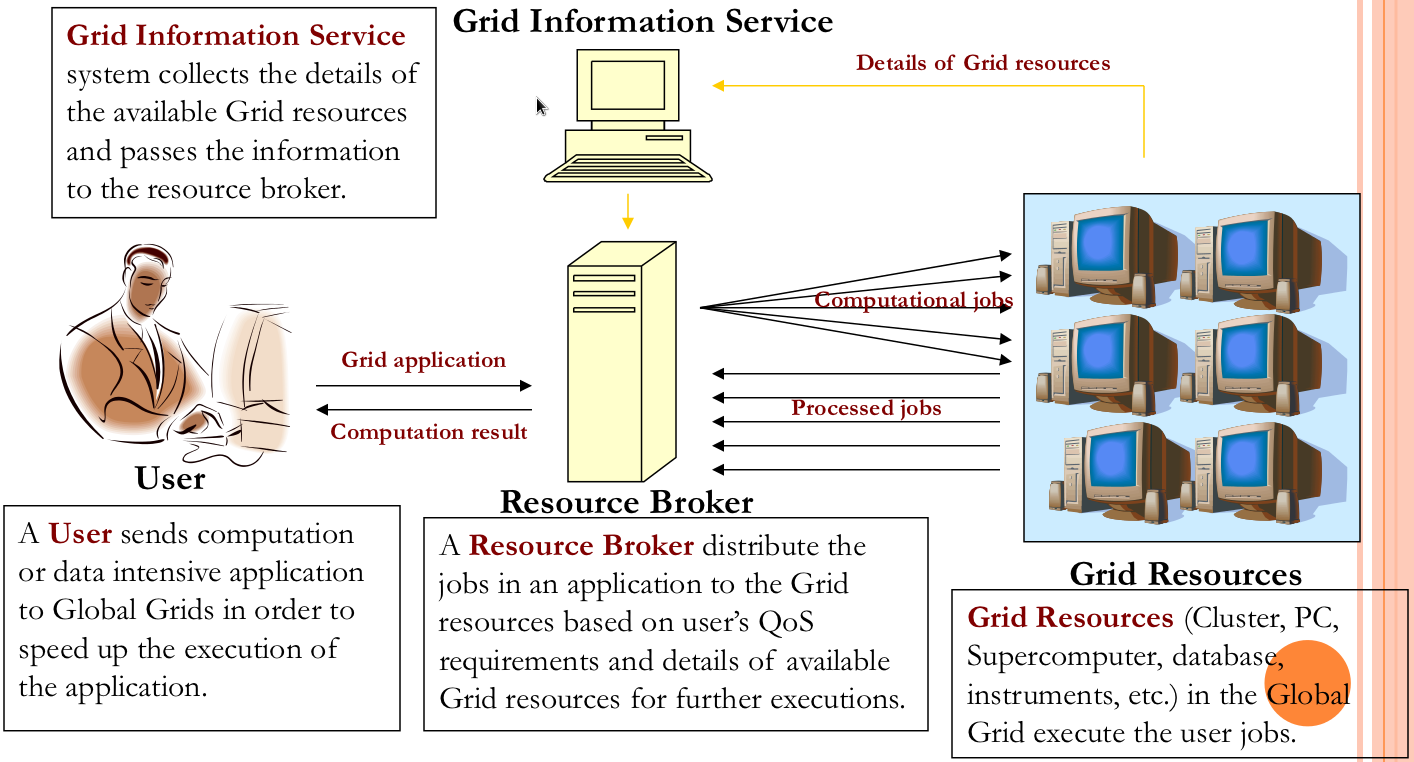
\includegraphics[width=0.95\textwidth]{imgs/gridenv}
\caption{A typical view of Grid environment}
\end{figure}
\end{frame}

\section[Problem Statement]{Problem Statement}
\begin{frame}[label=back3]
 \frametitle{Problem Statement}
\begin{itemize}
 	\item \textbf{Multi-objective dynamic scheduler in Grid}
	\begin{block}{1. Flexible Job Shop Scheduling} The typical job-shop problem is formulated as a work order that consists of set of $n$ jobs, each of which contains $m$ tasks and need to be scheduled on a set of resources with an objective of minimizing makespan.
	\end{block}
	\begin{itemize}
	\item Predecessor constraint: Each task has predecessors to complete before they can be executed.
	\item Resource constraint: Each task requires a certain type of resource to maintain their quality of service. 
	\end{itemize}
	\item Scheduling jobs on resources by considering multiple objectives in scenario is a challenging task. \hyperlink{multipleobj}{\beamerbutton{more}}
\end{itemize}
\end{frame}

\begin{frame}
 \frametitle{Problem Statement}
	\begin{block}{2. Real time dynamic scheduler} Dynamic scheduler considers dynamic environment of grid where resources can change its configuration and availability. In dynamic scheduling re-evaluation is allowed for already taken assignment decisions during job execution \cite{chtepen}.\\
	The grid must schedule jobs on resources as early as possible, giving scheduler few minutes to find a suitable strategy.\\
	\end{block}
\end{frame}
\begin{frame}
 \frametitle{Problem Statement}
	\begin{block}{3. Gridlet} Grid job is often referred to as Gridlet. Job characteristics e.g. job size varies widely making scheduler task difficult.\\
So, we need to provide a job grouping strategy for fine grained jobs for faster execution of scheduler. 
	\end{block}
\end{frame}

\section[Contributions]{Contributions}
\subsection*{Objectives}
\begin{frame}[label=multipleobj]
 \frametitle{Contributions}
 \begin{itemize}
	\item We present a multi-objective job scheduler based on Genetic Algorithm which considers following objectives
	\begin{itemize}
	 \item Minimize makespan
	 \item Maximum utilization
	 \item Energy efficient schedule
	 \item Minimization of Time penalty
	 \item Minimization of Cost penalty
	\end{itemize}
	\item This provide grid administrator a better grip on the trade off among cost, time limit, energy, performance.\hyperlink{back3}{\beamerbutton{back}}
\end{itemize}
\end{frame}

\subsection*{Non-dominating approach}
\begin{frame}[label=back4]
 \frametitle{Contributions (contd.)}
 \begin{itemize}
	\item Pareto front approach (unlike weighted sum) for optimizing each objective separately in each generation of GA \hyperlink{paretofrnt}{\beamerbutton{more}}.
	\item Non dominated sorting with elitist mechanism to preserve good scheduling strategies during transition of generation \hyperlink{nds}{\beamerbutton{more}}.
	\item Avant-garde crossover and mutation operators to explore search space minutely and still fast enough to produce near optimal solution in real time.
\end{itemize}
\end{frame}

\subsection*{Dynamic scheduler}
\begin{frame}
 \frametitle{Contributions (contd.)}
 \begin{itemize}
	\item Dynamic scheduler; resources leaving or joining grid environment triggers rescheduling of jobs.
	\item Job grouping strategy with predecessor and resource constraint.
\end{itemize}
\end{frame}


\section[Approach]{Proposed Approach}
\begin{frame}
 \frametitle{Scheduling model}
\begin{figure}[t]
\centering
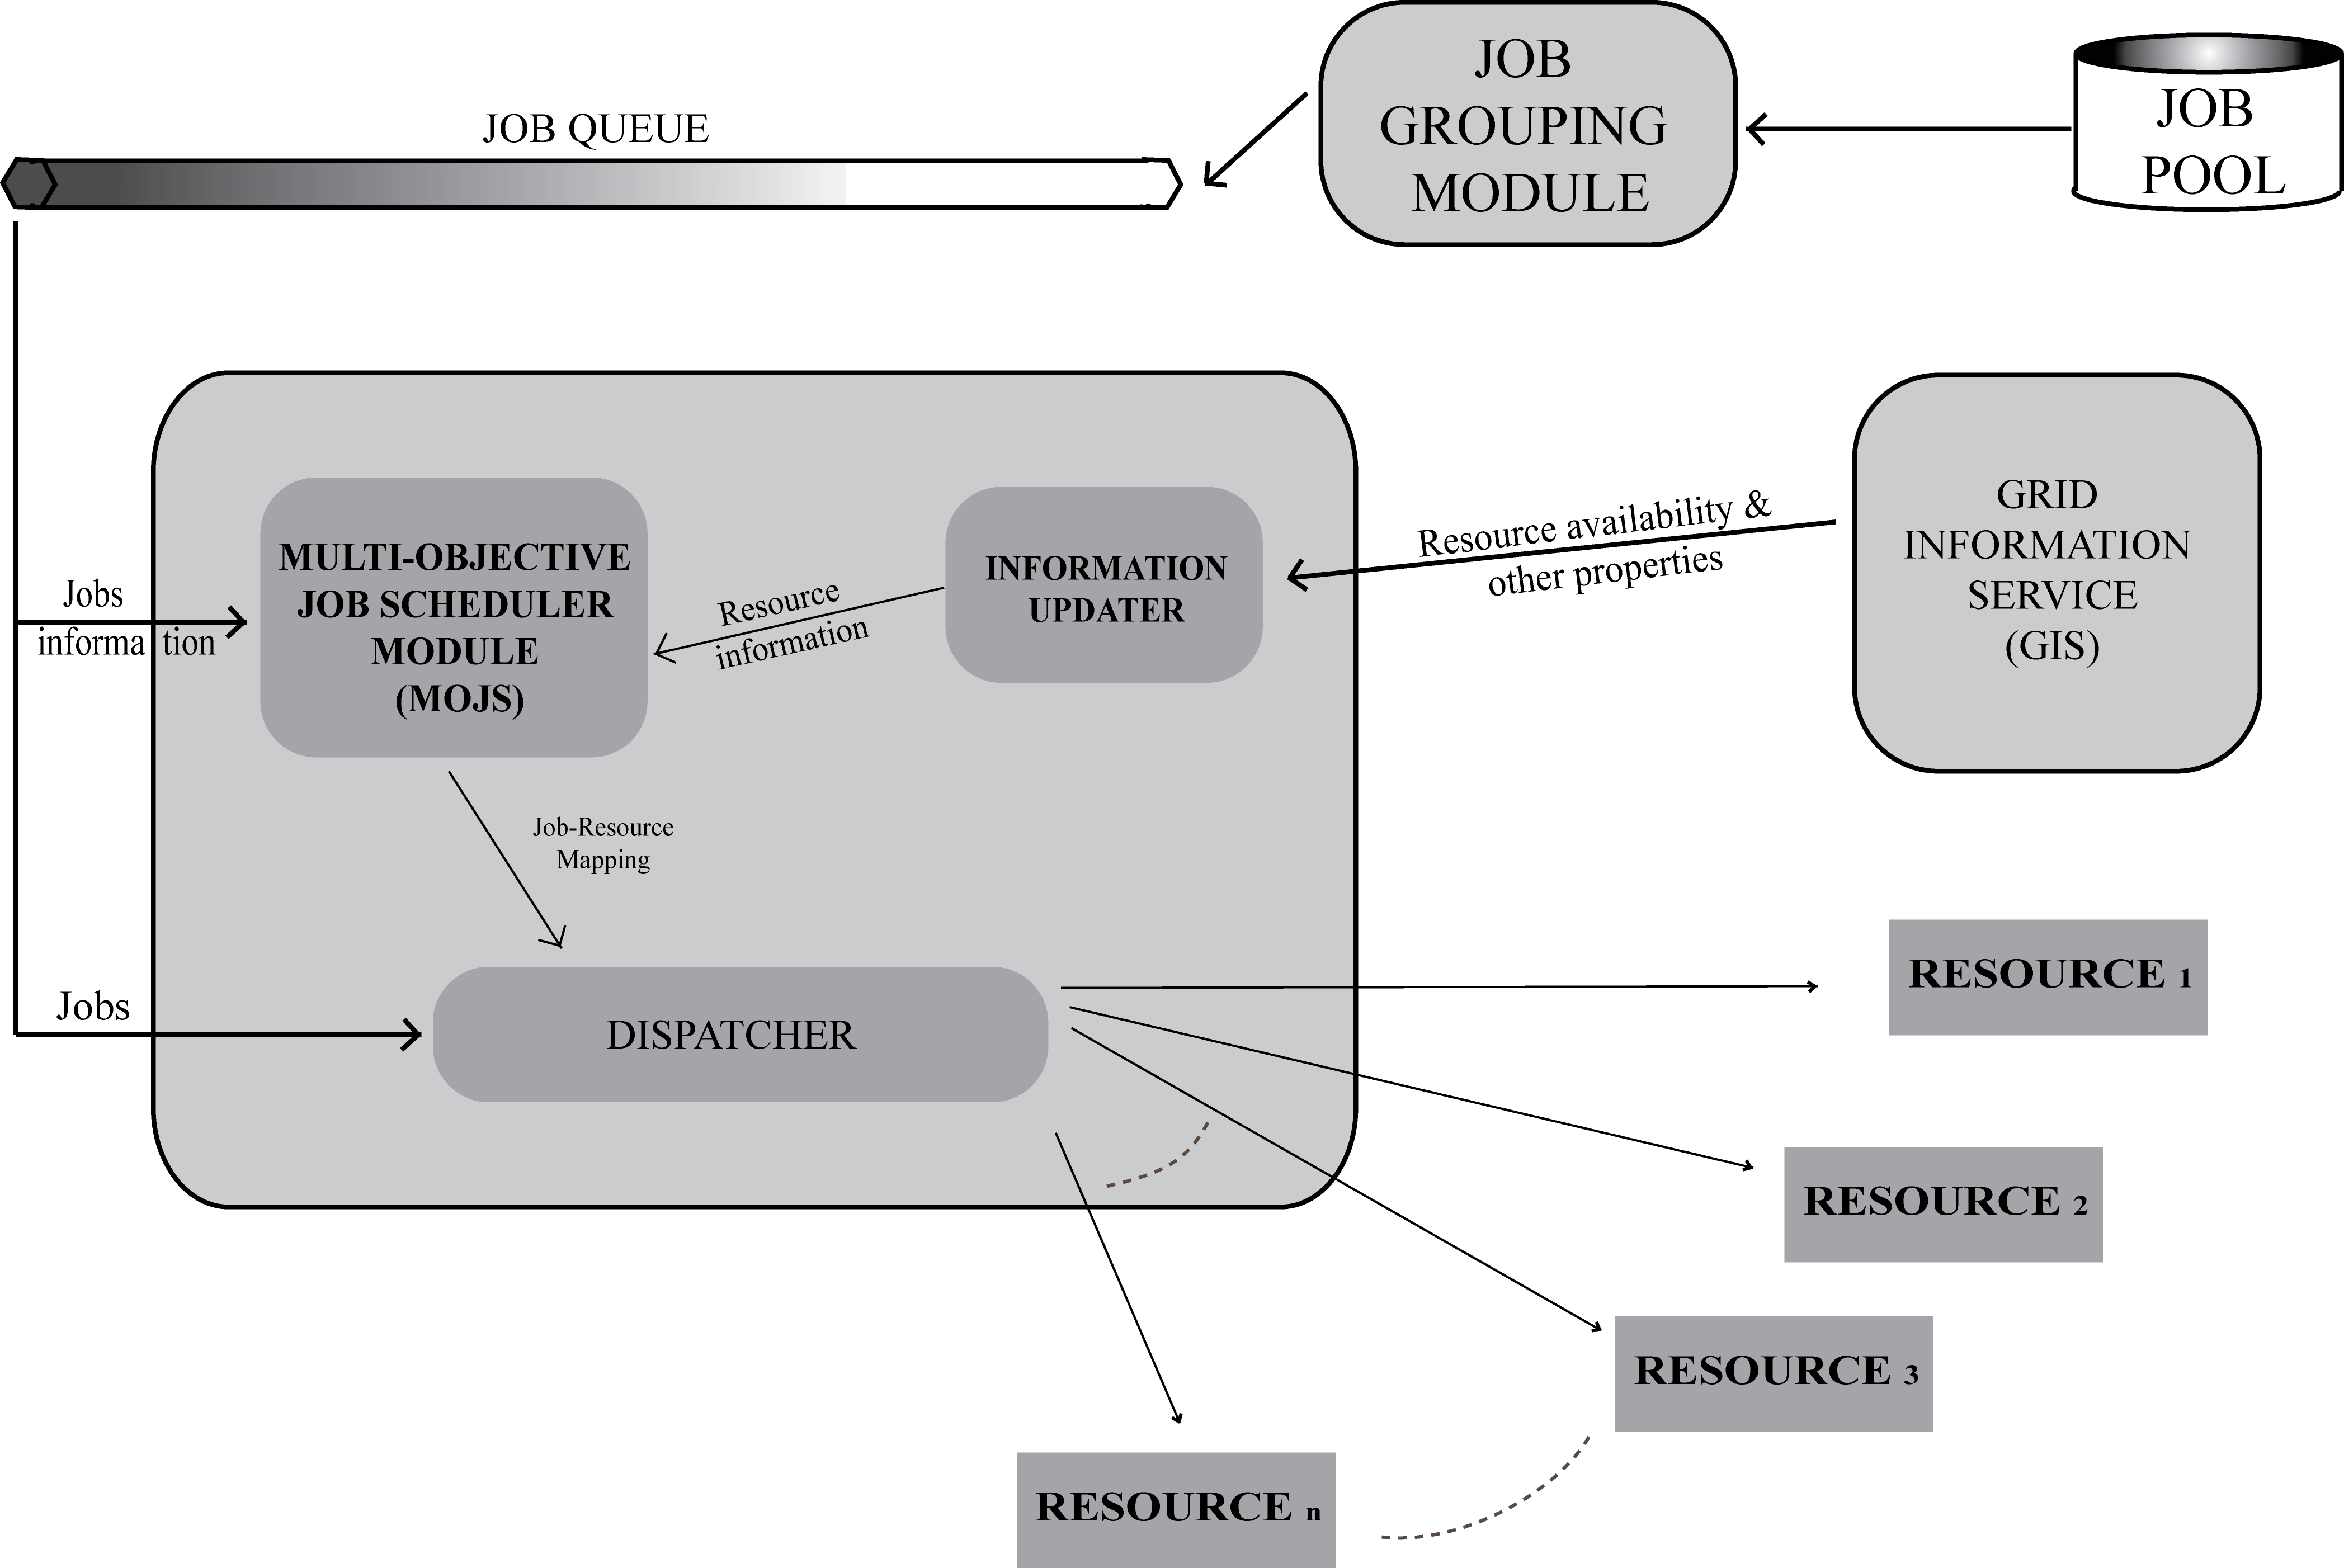
\includegraphics[width=0.80\textwidth]{imgs/scheduler}
%\caption{Scheduling Model}
\end{figure}
\end{frame}

\subsection*{Formulation of problem}
\begin{frame}
\frametitle{Formulation of problem}
  \begin{itemize}
  \item Given are a set $M = \{M_1, M_2, M_3, ... M_m\}$ of resources.
  \item A set $J = \{J_1, J_2, J_3, ... J_j\}$ of application jobs, and a set $O$ of grid jobs.
  \item $n$ Grid jobs of application job $J_i$ are denoted by $O_{i1},..., O_{in}$.
  \item A set $W= \{W_1,W_2,\ldots,W_m\}$ denotes normalized energy dissipation factor of resources.
  \end{itemize}
\end{frame}

\begin{frame}[label=notation]
\frametitle{Notations}
\begin{table}[!ht]
\caption{Notations and their definitions}
\centering
\scalebox{0.65}{
    \begin{tabular}{|c|l|}
    \hline \hline
    Notation & Definition  \\ \hline
    $M_i$ & Resource with ID $i$ \\ \hline
    $J_i$ & Application job with ID $i$ \\ \hline
    $O_{ij}$ & $j$th Grid Job or task of Application job $J_i$ \\ \hline
    $W_i$ & Energy dissipation factor of Resource $M_i$, \\
	  & normalized with the max value from set $W$ \\ \hline
    $t(O_{ij},R_{ij})$ & Processing time of $O_{ij}$ mapped to resource $R_{ij}$ \\ \hline
    $c(O_{ij},R_{ij})$ & Cost of $O_{ij}$ mapped to resource $R_{ij}$ \\ \hline
    $s(O_{ij})$ & Start time of job $O_{ij}$ \\ \hline
    $e(O_{ij})$ & End time of job $O_{ij}$ \\ \hline
    $d_{ij}$ & Time limit for completion of $O_{ij}$ \\ \hline
    $c'_{ij}$ & cost limit for  $O_{ij}$ \\ \hline
    $tsum(M_i)$ & Running time or Uptime of $M_i$ \\ \hline
    \end{tabular}
}
\end{table}
\end{frame}


\begin{frame}
\frametitle{Restrictions}
A schedule strategy is valid, if the following two \textbf{restrictions} are met:
\begin{enumerate}
  \item All grid jobs are planned and resources are allocated exclusively:
  \begin{itemize}
    \item $ \forall O_{ij} : \exists s(O_{ij}) \in \mathbb{R}, R_{ij} \in \mu_{ij} : \forall M_j \in R_{ij} $:
    \item $M_j$ is in $[s(O_{ij});s(O{ij})+t(O_{ij}),R_{ij}]$ exclusively allocated by $O_{ij}$
  \end{itemize}
  \item Precedence relations are adhered to: 
  \begin{itemize}
    \item $\forall i, j \neq k : p(O_{ij},O_{ik}) \Rightarrow s(O_{ik}) \geq s(O_{ij}) +t(O_{ij}, R_{ij})$
  \end{itemize}
\end{enumerate}
\end{frame}


\begin{frame}
\frametitle{Soft constraints}
Exceeding the time limit and budget cost will affect QoS of grid jobs. A penalty factor is imposed when jobs violates following \textbf{constraints}.
\begin{enumerate}
  \item All grid jobs $O_{ij}$ have time limit $d_{ij}$ which must be adhered to:
  \begin{itemize}
   \item $ \forall O_{ij} : d_{ij} \geq s(O_{ij}) + t(O_{ij},R_{ij}) $:
  \end{itemize}
  \item All grid jobs $O_{ij}$ have a cost limit  $c'_{ij}$ which must be adhered to: 
  \begin{itemize}
   \item $\forall O_{ij} : c'_{ij} \geq c(O_{ij},R_{ij}) $
  \end{itemize}
\end{enumerate}
\end{frame}

\begin{frame}[label=mkspn1]
\frametitle{Objective functions or fitness functions}
This work focuses on achieving near-optimal scheduling strategy on following objective functions
\begin{enumerate}
  \setcounter{enumi}{0}
  \item Minimizing makespan, $e(O_{ij})$ is the end time of grid job $O_{ij}$
  \begin{itemize}
   \item $ f_1 =makespan = max\{e(l(M_1)),e(l(M_2)),\ldots,e(l(M_m)) \}$
      \begin{block}
      {Makespan} It is the time at which all the resources becomes free \hyperlink{supplement1}{\beamerbutton{defn}}.
      \end{block}
  \end{itemize}
  \item Maximizing utilization of resources i.e. minimizing $f_2$
  \begin{itemize}
  \item $ f_2 = non-utilization = \frac{1}{m} \sum_{j=1}^{m}  \{e(l(M_j)) - tsum (M_j)\}$
  \end{itemize}
\end{enumerate}
\end{frame}

\begin{frame}
\frametitle{Objective functions or fitness functions (contd.)}
\begin{enumerate}
  \setcounter{enumi}{2}
  \item Minimizing time limit penalty (minimizing number of jobs completing after due date)
$$
f_3 = \frac{1}{j*n}  \sum_{\forall i,j} \varphi _1 (e(O_{ij}) - d_{ij}) 
$$
where $\varphi _1(x)$ is a non-negative continuous exponential non-decreasing function, if $x > 0$ else $0$.
\begin{block}{Time penalty}
The grid jobs failed to complete within time limit contribute to the penalty function $f_3$. Minimizing time limit penalty is our aim.
\end{block}
\end{enumerate}
\end{frame}

\begin{frame}
\frametitle{Objective functions or fitness functions (contd.)}
\begin{enumerate}
  \setcounter{enumi}{3}
  \item Minimizing cost penalty 
$$
f_4 = \frac{1}{j*n}  \sum_{\forall i,j} \varphi _2 \{c(O_{ij},R_{ij}) - c'_{ij}\} 
$$
where $\varphi _2(x)$ is a non-negative continuous linear non-decreasing function, if $x > 0$ else $0$.
  \item Minimizing Overall Energy consumption
  \begin{itemize}
  \item $f_5 = \sum_{i=1}^{m} tsum(M_i) * W_i$
  \vspace{5pt}
  \item $f_5$ is the energy consumption of all the resources.
  \end{itemize}
\end{enumerate}
\end{frame}

\subsection*{Flowchart}
\begin{frame}
\frametitle{MOJS flowchart}
\begin{figure}[t]
\centering
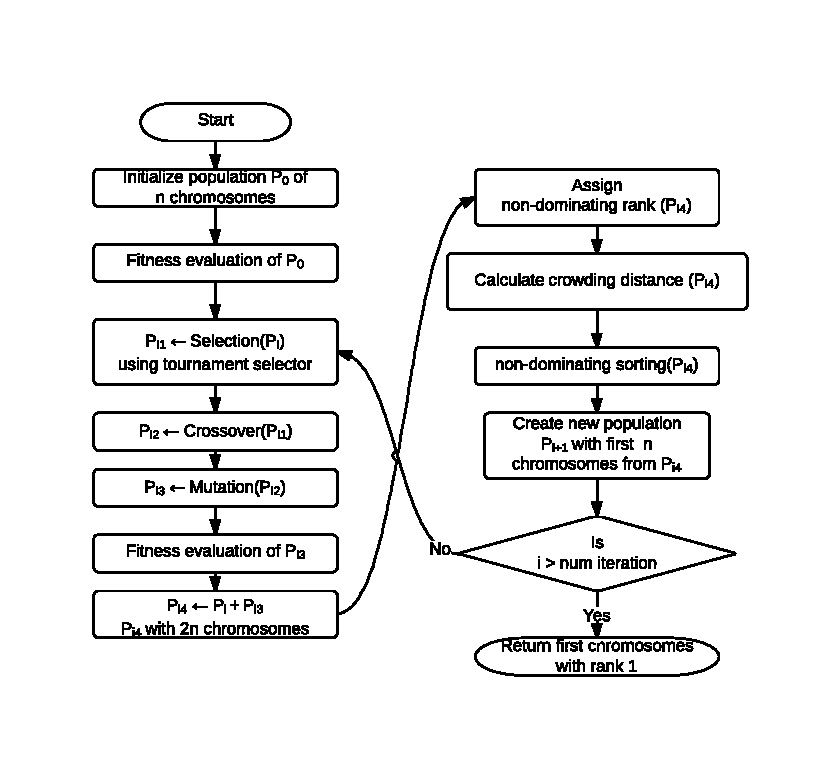
\includegraphics[width=0.62\textwidth]{imgs/GA}
%\caption{MOJS algorithm}
\end{figure}
\end{frame}

\begin{frame}
\frametitle{Schematic overview}
\begin{figure}[t]
\centering
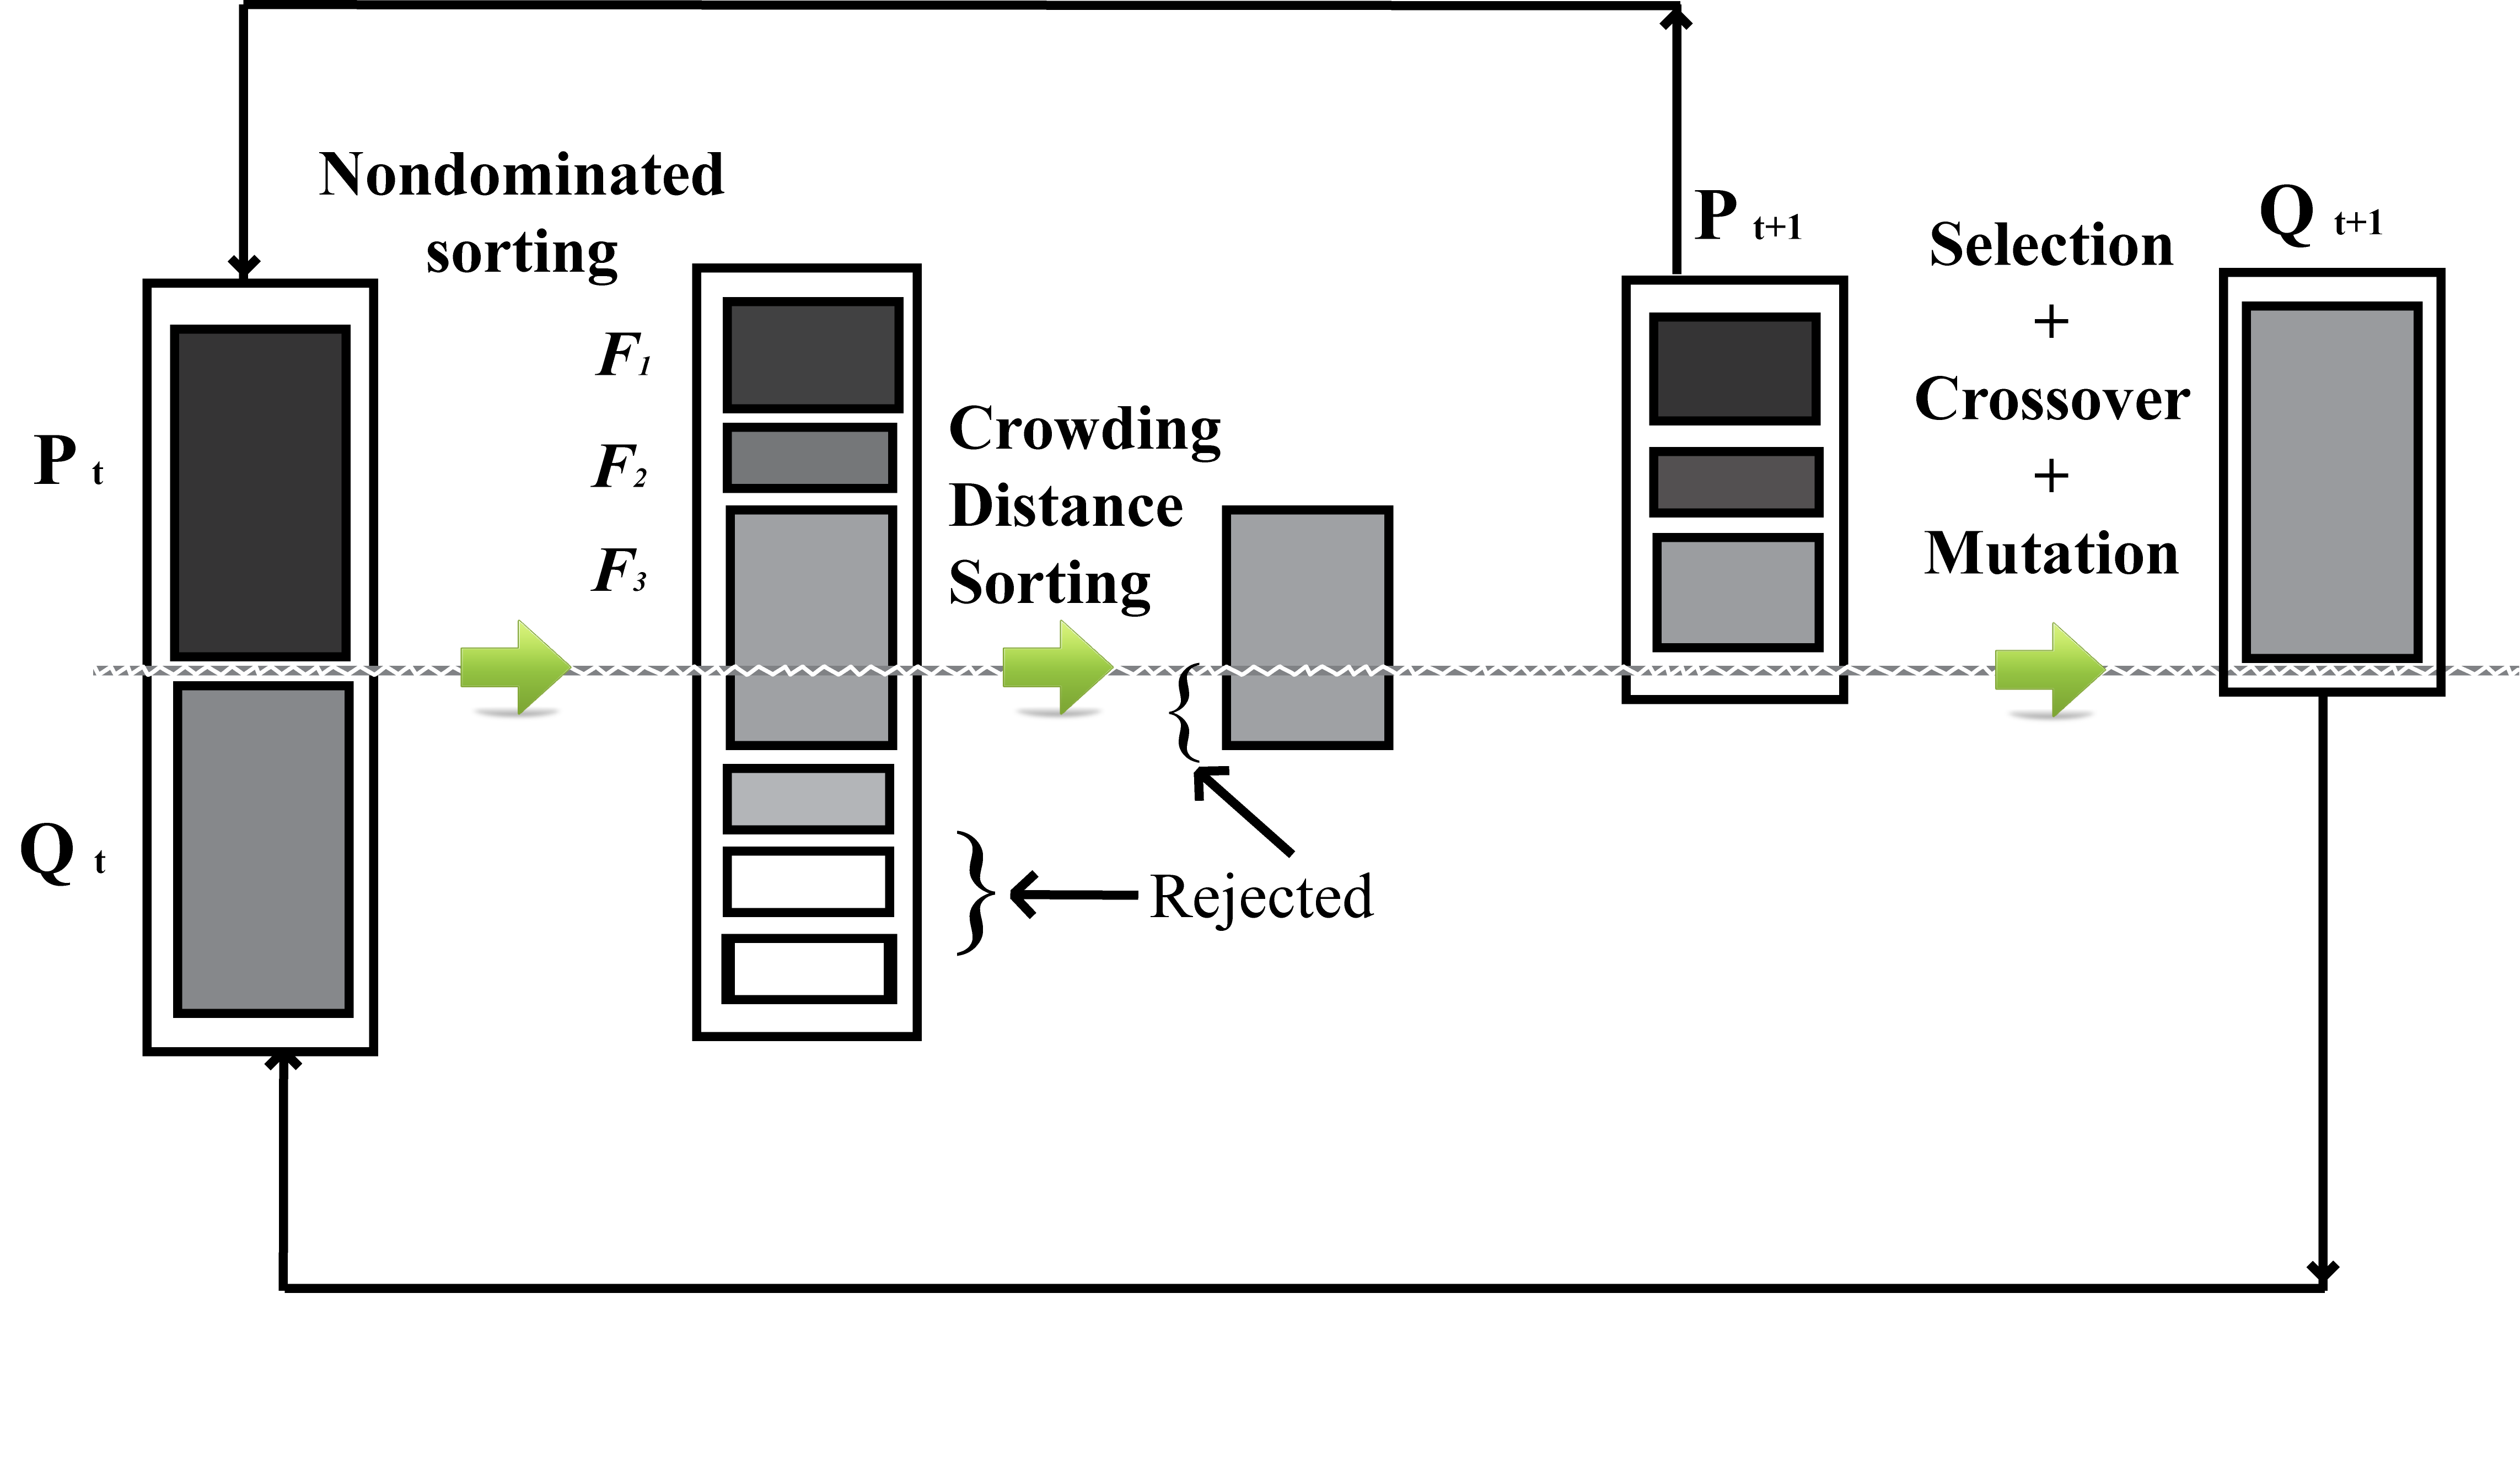
\includegraphics[width=0.80\textwidth]{imgs/NSGA2}
%\caption{MOJS algorithm}
\end{figure}
\end{frame}


\subsection*{Chromosome model}
\begin{frame}[label=chromosomemod] 
\frametitle{Chromosome model}
\begin{itemize}
\item A scheduling strategy $\leftrightarrow$  A chromosome. 
\begin {itemize}
\item Resource id corresponding to each job
\item Start time of every job
\item End time of every job
\item Predecessor job ID of each job 
\item Five objective function values 
\item Rank of chromosome \hyperlink{nds1}{\beamerbutton{more}}.
\item Crowding distance \hyperlink{crwd}{\beamerbutton{more}}.
\end{itemize}
\item Start time for execution of jobs is calculated according to heuristic rules
\begin{enumerate}
 \item Schedule grid job as early as its precedent job is completed.
 \item Schedule grid jobs according to shortest due date.
\end{enumerate}
\end{itemize}
\end{frame}

\subsection*{Crossover}
\begin{frame}
\frametitle{Crossover operators: k-point crossover}
\begin{figure}[!h]
    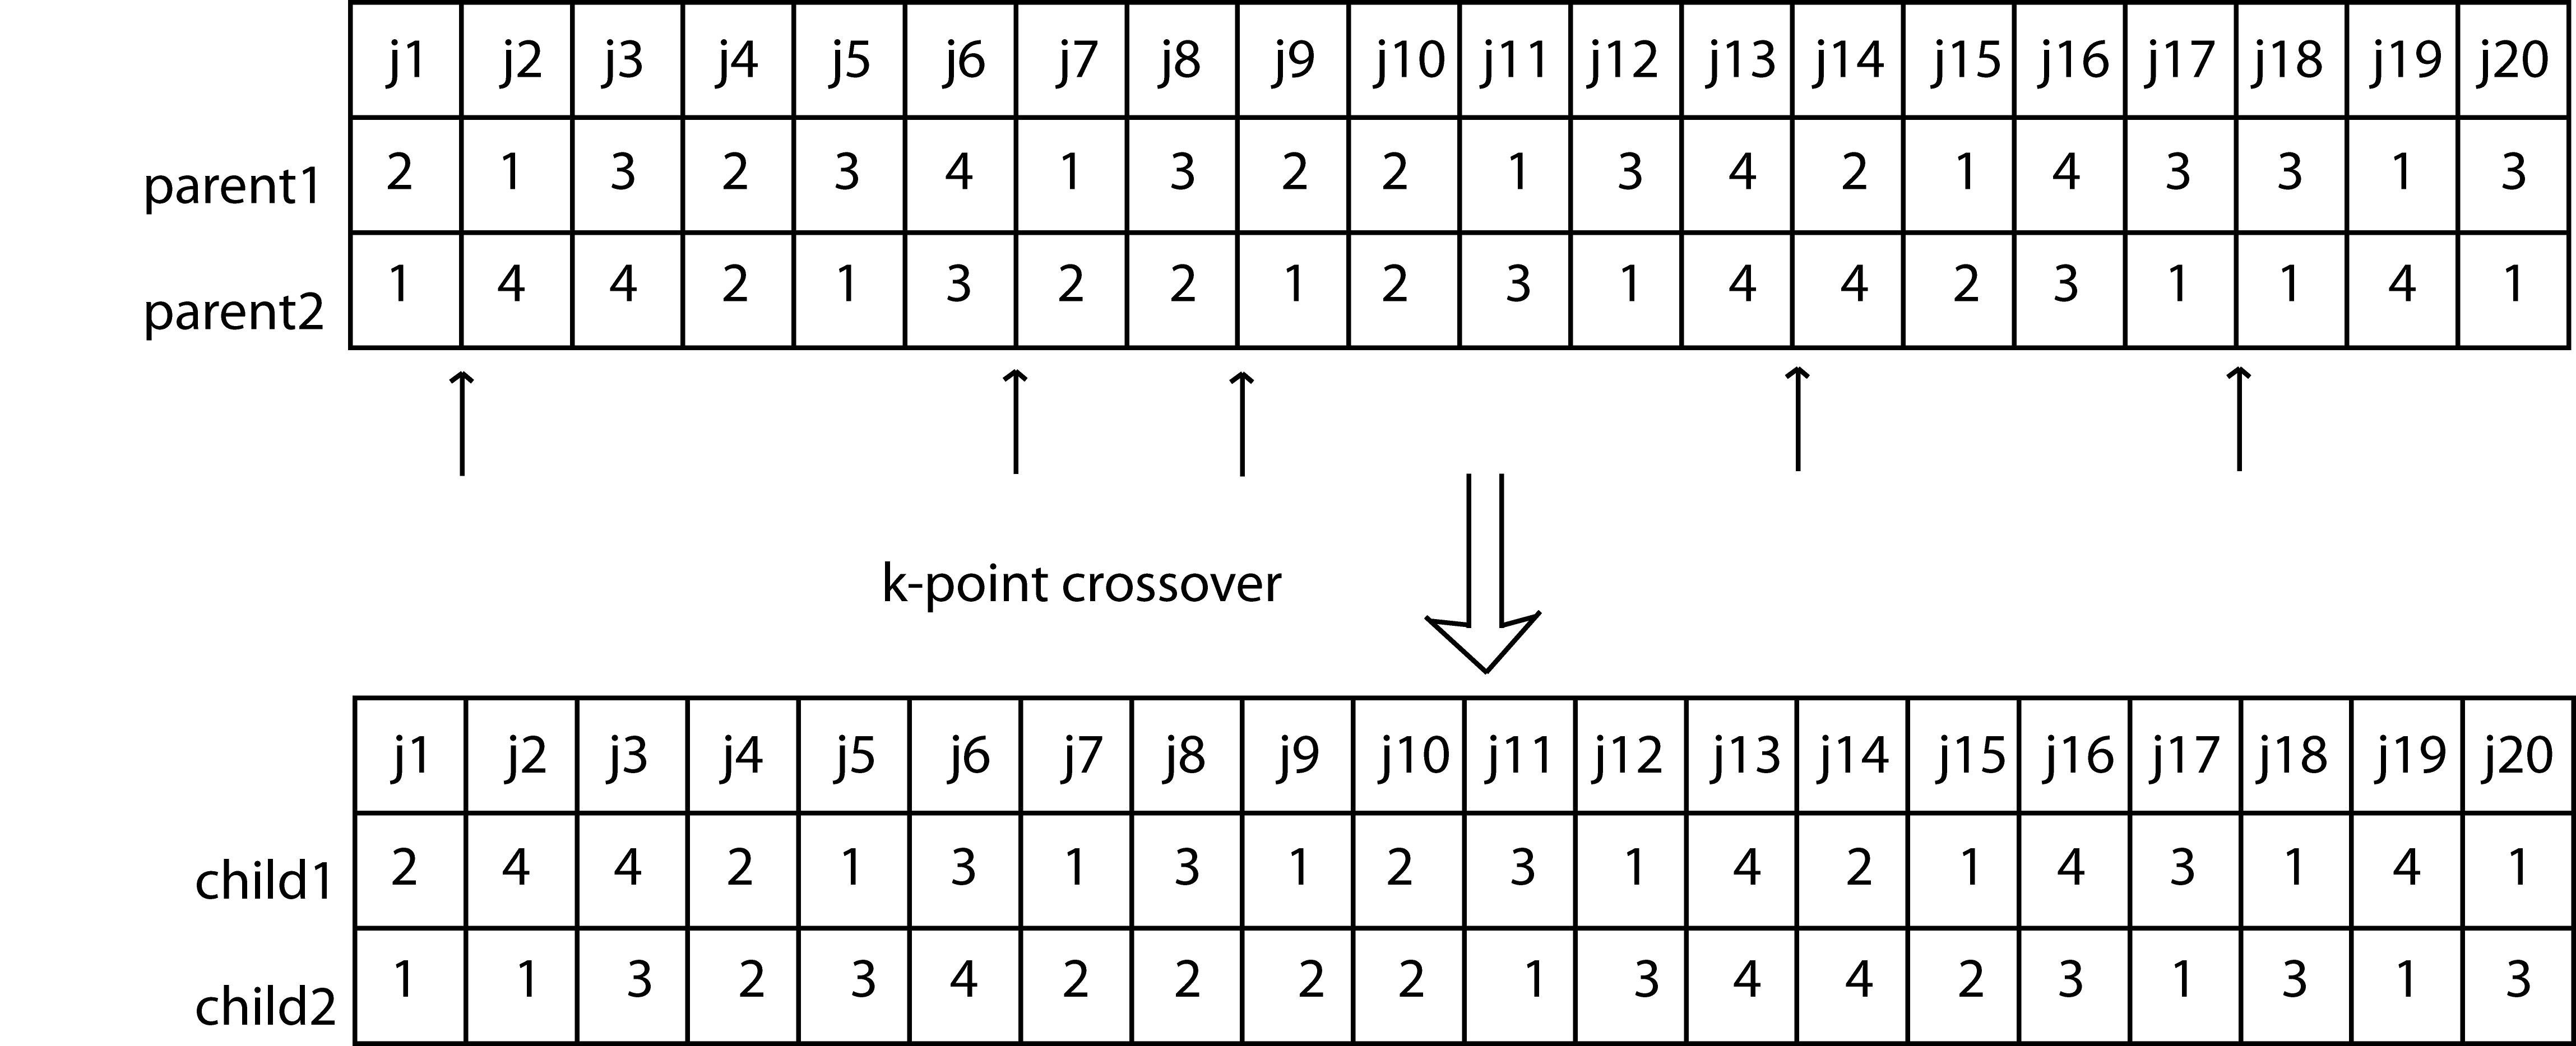
\includegraphics[width=\textwidth]{imgs/crossover2}
    \caption{k-point crossover}
\end{figure}
\end{frame}

\begin{frame}
\frametitle{Crossover operators: Mask crossover}
\begin{figure}[!h]
    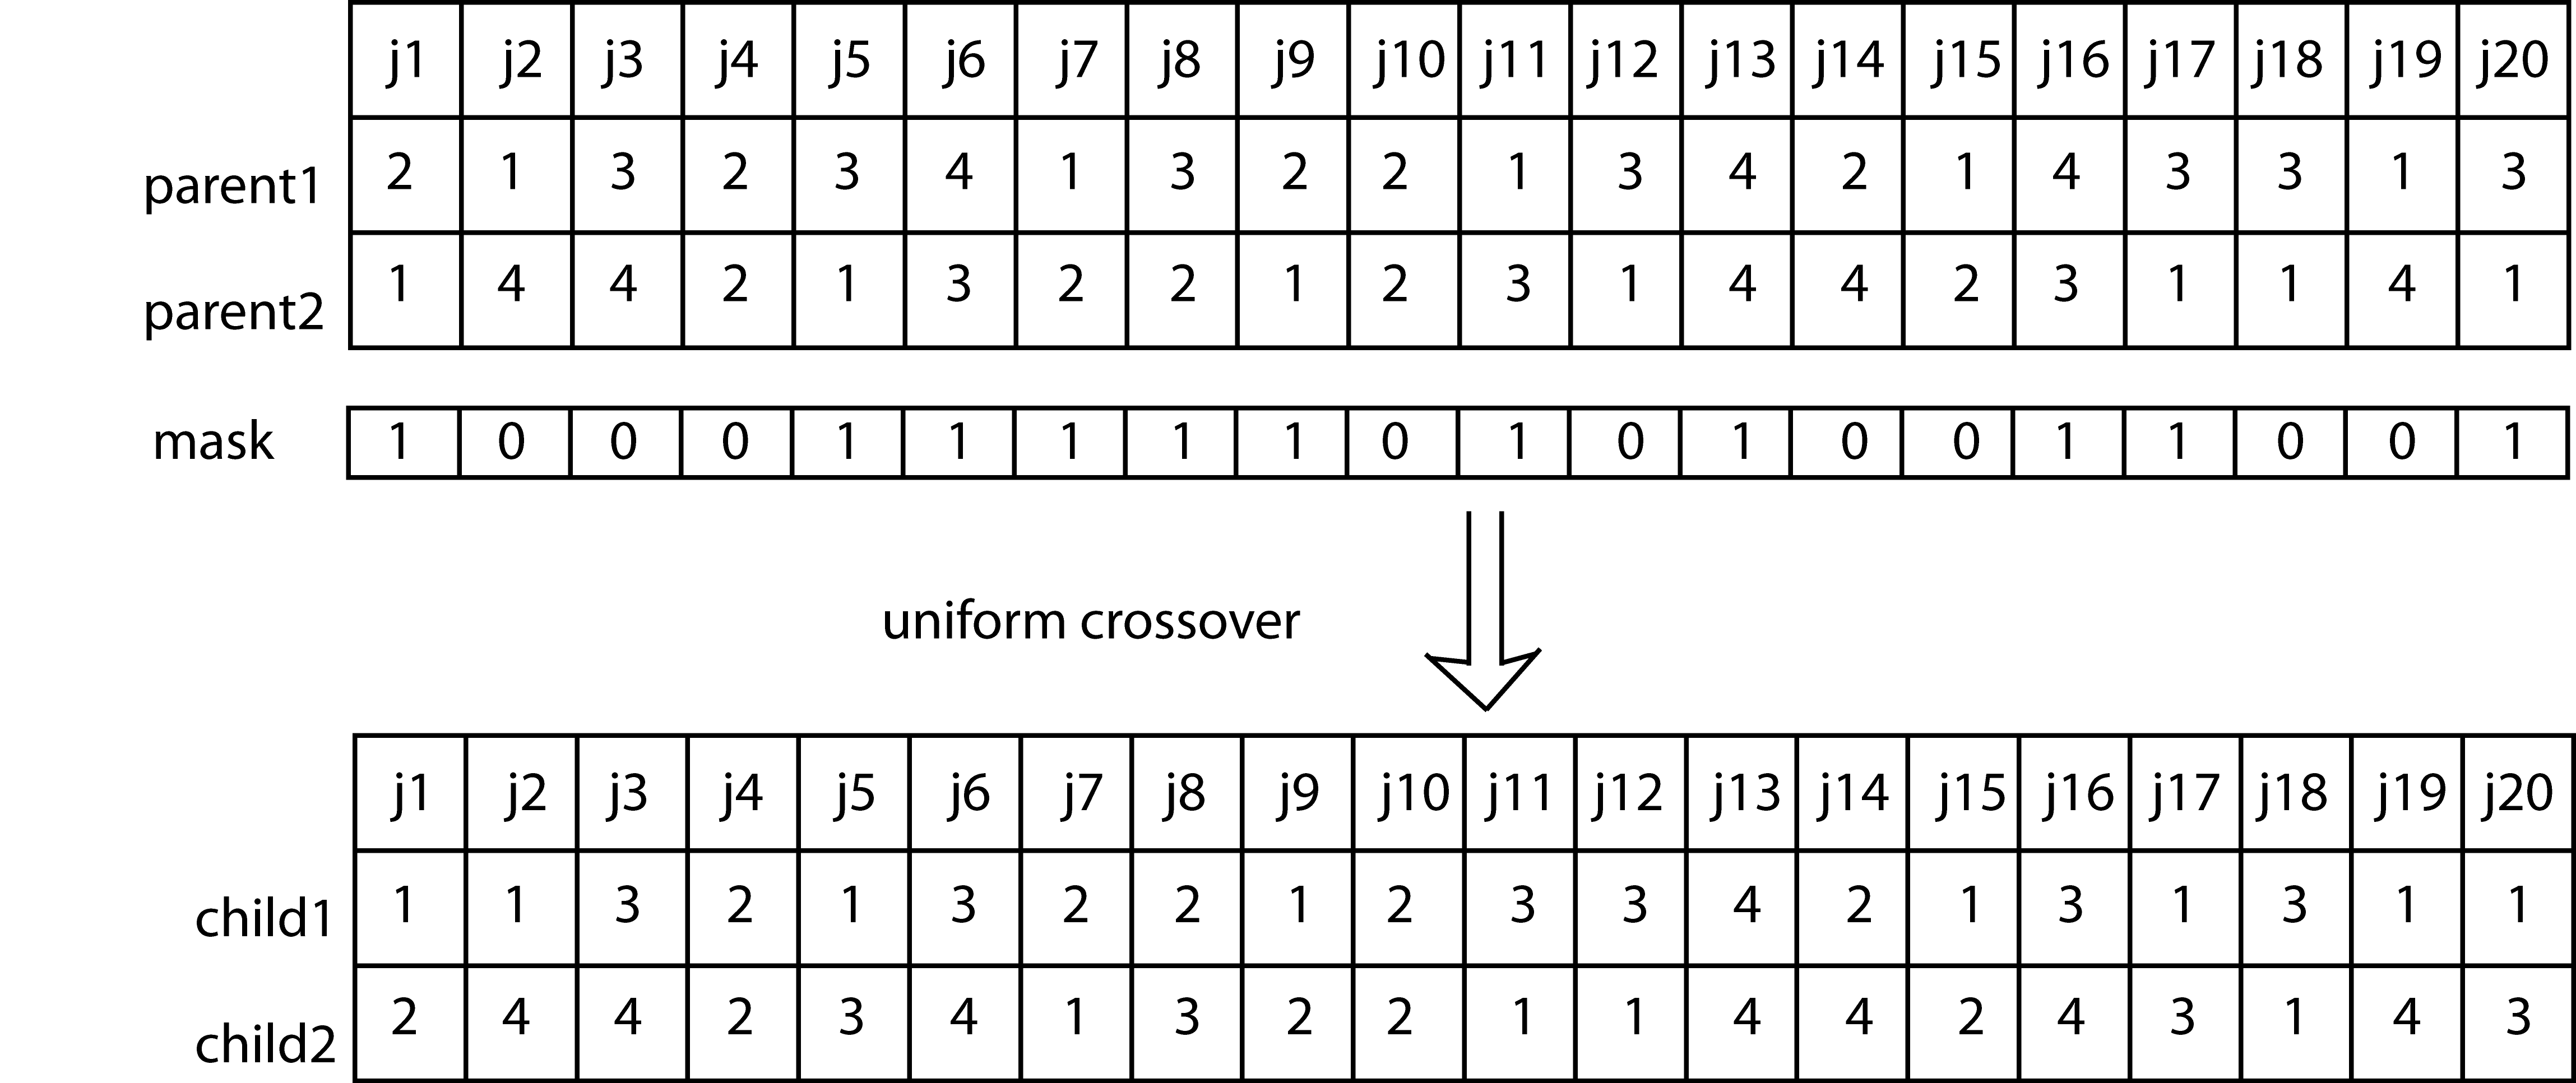
\includegraphics[width=\textwidth]{imgs/crossover3}
    \caption{Mask crossover}
\end{figure}
\end{frame}
\begin{frame}
 \frametitle{Crossover operators: Fitness based crossover}
{\small
\begin{itemize}
\item $g_1[i], g_2[i]$ are energy efficiency parameter of $chromosome_{parent_1}[i]$ and $chromosome_{parent_2}[i]$ respectively.
\end{itemize}
}
{\tiny
\begin{align}
\forall i, chromosome_{new_1}[i] = \left\{ \begin{array}{rl}
 chromosome_{parent_1}[i] &\mbox{with probability $p = \frac{g_1[i]}{g_1[i] +g_2[i]}$} \\
 chromosome_{parent_2}[i] &\mbox{with probability $1-p$}
       \end{array} \right.
\end{align}
}
{\tiny
\begin{align}
\forall i, chromosome_{new_2}[i] = \left\{ \begin{array}{rl}
 chromosome_{parent_1}[i] &\mbox{with probability $p = \frac{h_1[i]}{h_1[i] +h_2[i]}$} \\
 chromosome_{parent_2}[i] &\mbox{with probability $1-p$}
       \end{array} \right.
\end{align}
}
{\small
\begin{itemize}
\item $h_1[i], h_2[i]$ are processing capability parameter of $chromosome_{parent_1}[i]$ and $chromosome_{parent_2}[i]$ respectively.
\end{itemize}
}
\end{frame}
\begin{frame}
\frametitle{Crossover operators: Fitness based crossover}
\begin{figure}[!h]
    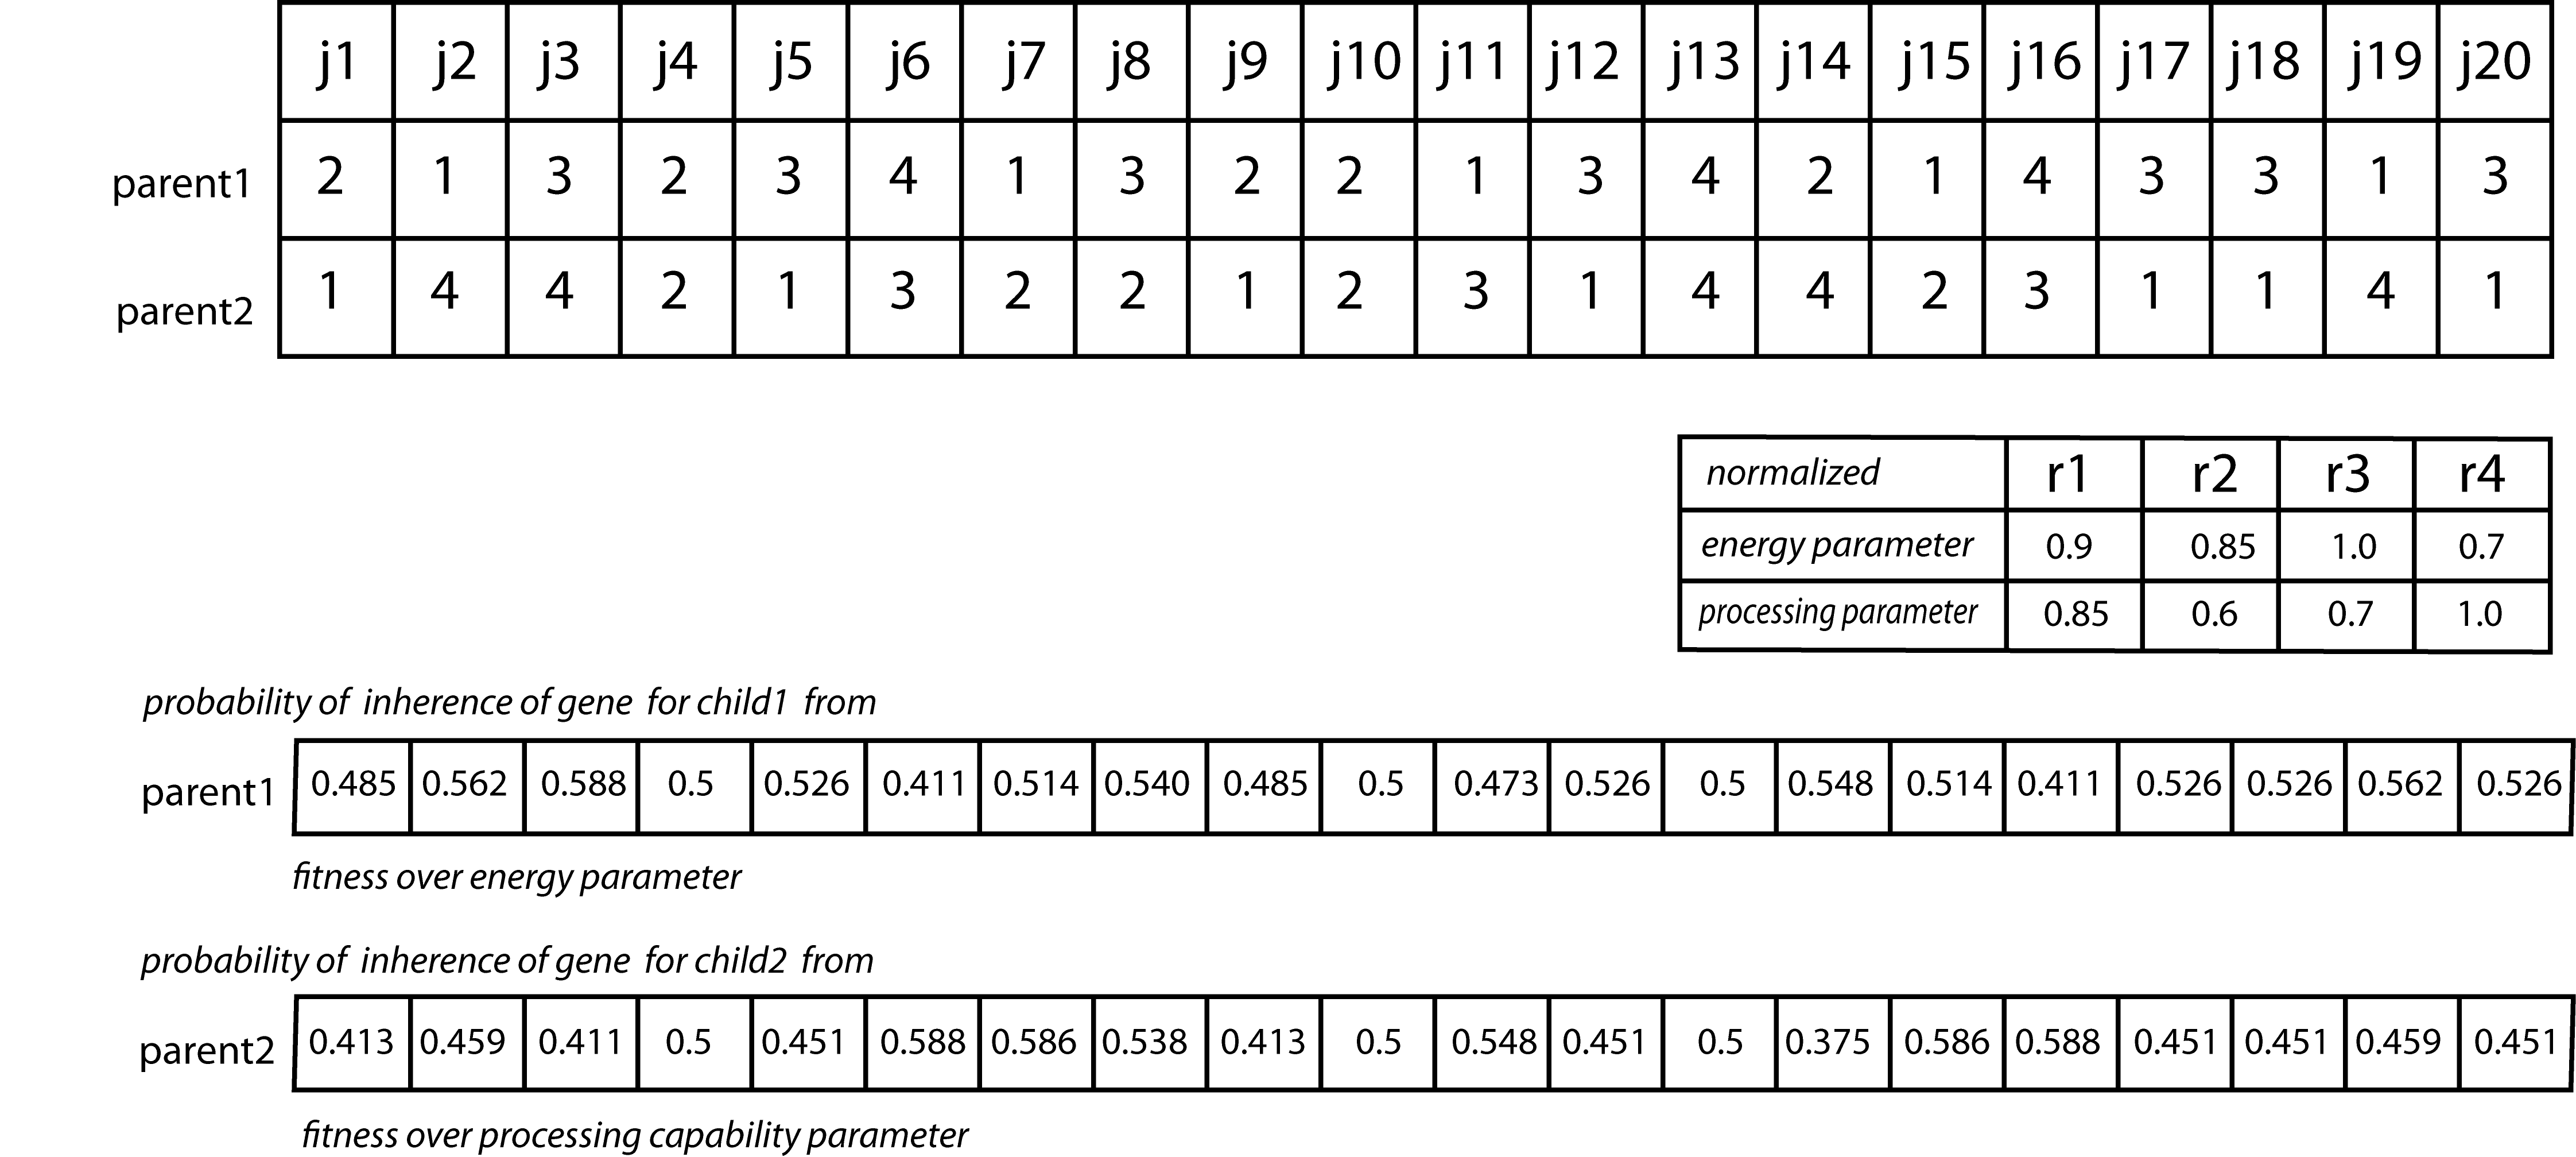
\includegraphics[width=\textwidth]{imgs/crossover5}
    \caption{Fitness based crossover}
\end{figure}
\end{frame}

\subsection*{Mutation}
\begin{frame}
\frametitle{Mutation operators: Move}
\begin{figure}[!h]
    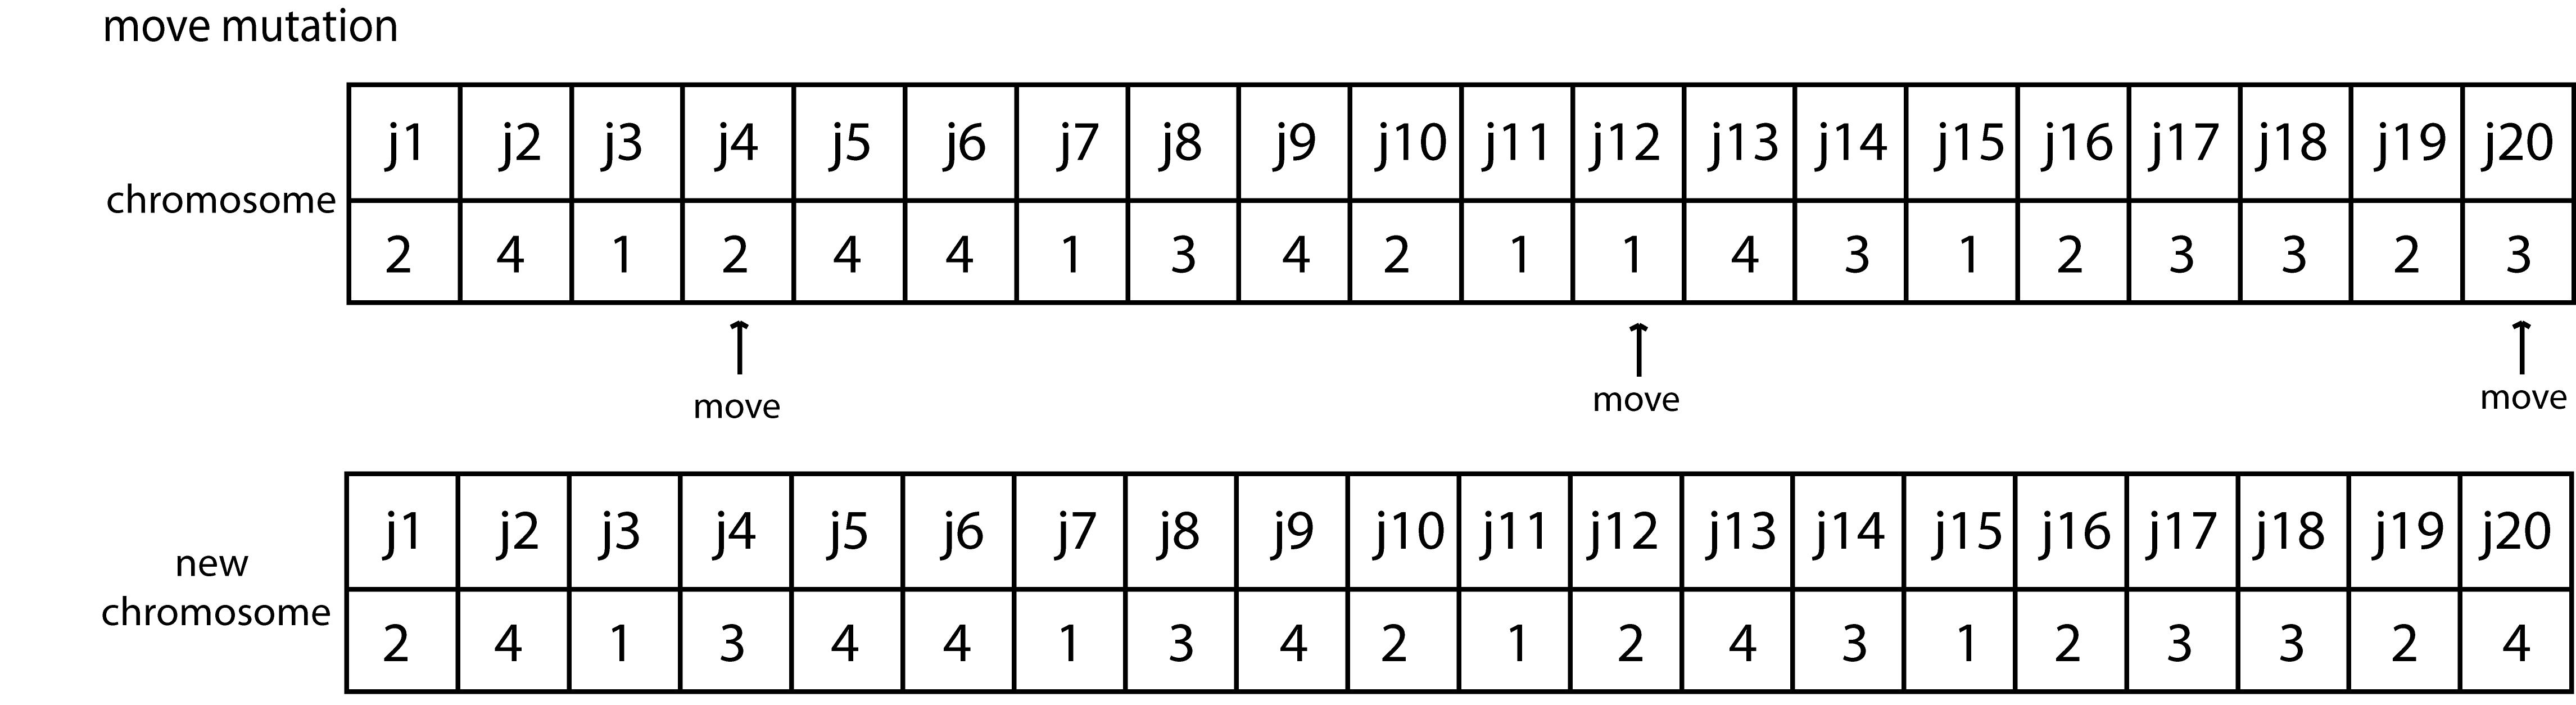
\includegraphics[width=\textwidth]{imgs/mutation1}
    \caption{Mutation- move}
\end{figure}
\end{frame}

\begin{frame}
\frametitle{Mutation operators: Swap}
\begin{figure}[h]
    \centering
    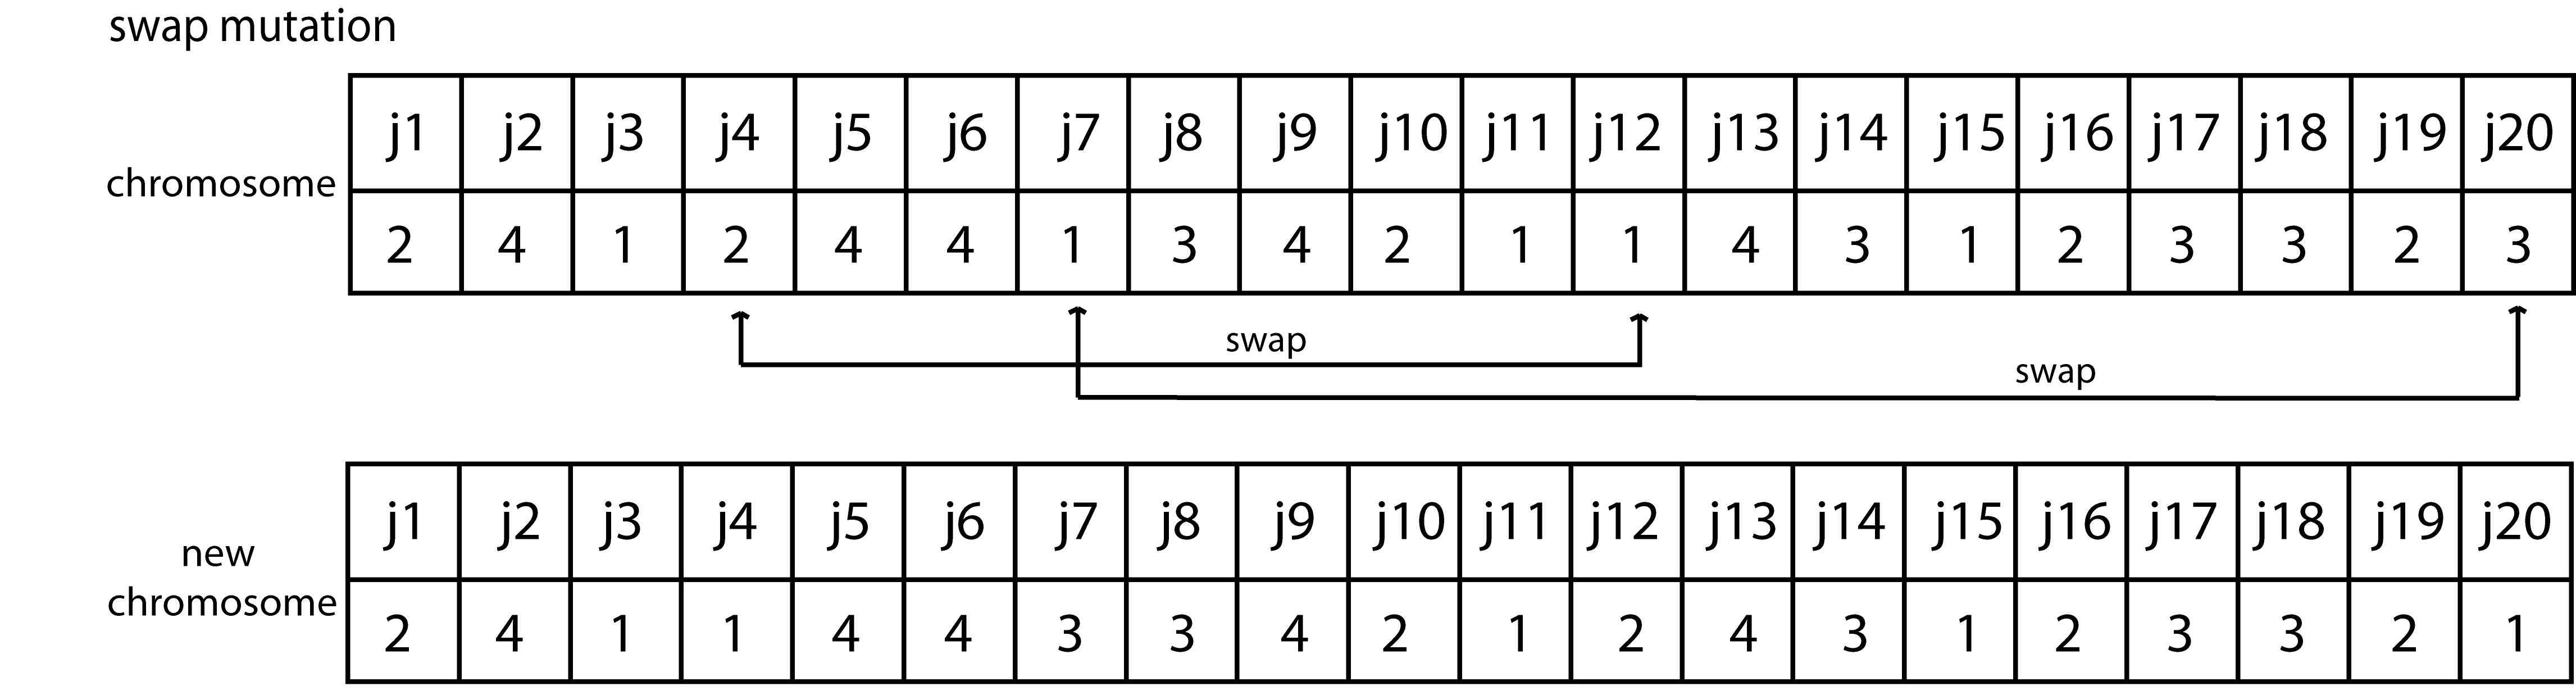
\includegraphics[width=\textwidth]{imgs/mutation2}
    \caption{Mutation- swap}
\end{figure}
\end{frame}

\begin{frame}
\frametitle{Mutation operators: Rebalancing}
\begin{itemize}
 \item This operator takes into account number of jobs assigned to each resource. It chooses most overloaded resource and randomly pick a job assigned to it. Then the job is moved to a resource which is less overloaded.
\end{itemize}
\end{frame}

\subsection*{Job grouping}
\begin{frame}[label=jbgrpimg]
\frametitle{Job grouping \hyperlink{jbgrp}{\beamerbutton{algorithm link}}}
\begin{figure}[h]
    \centering
    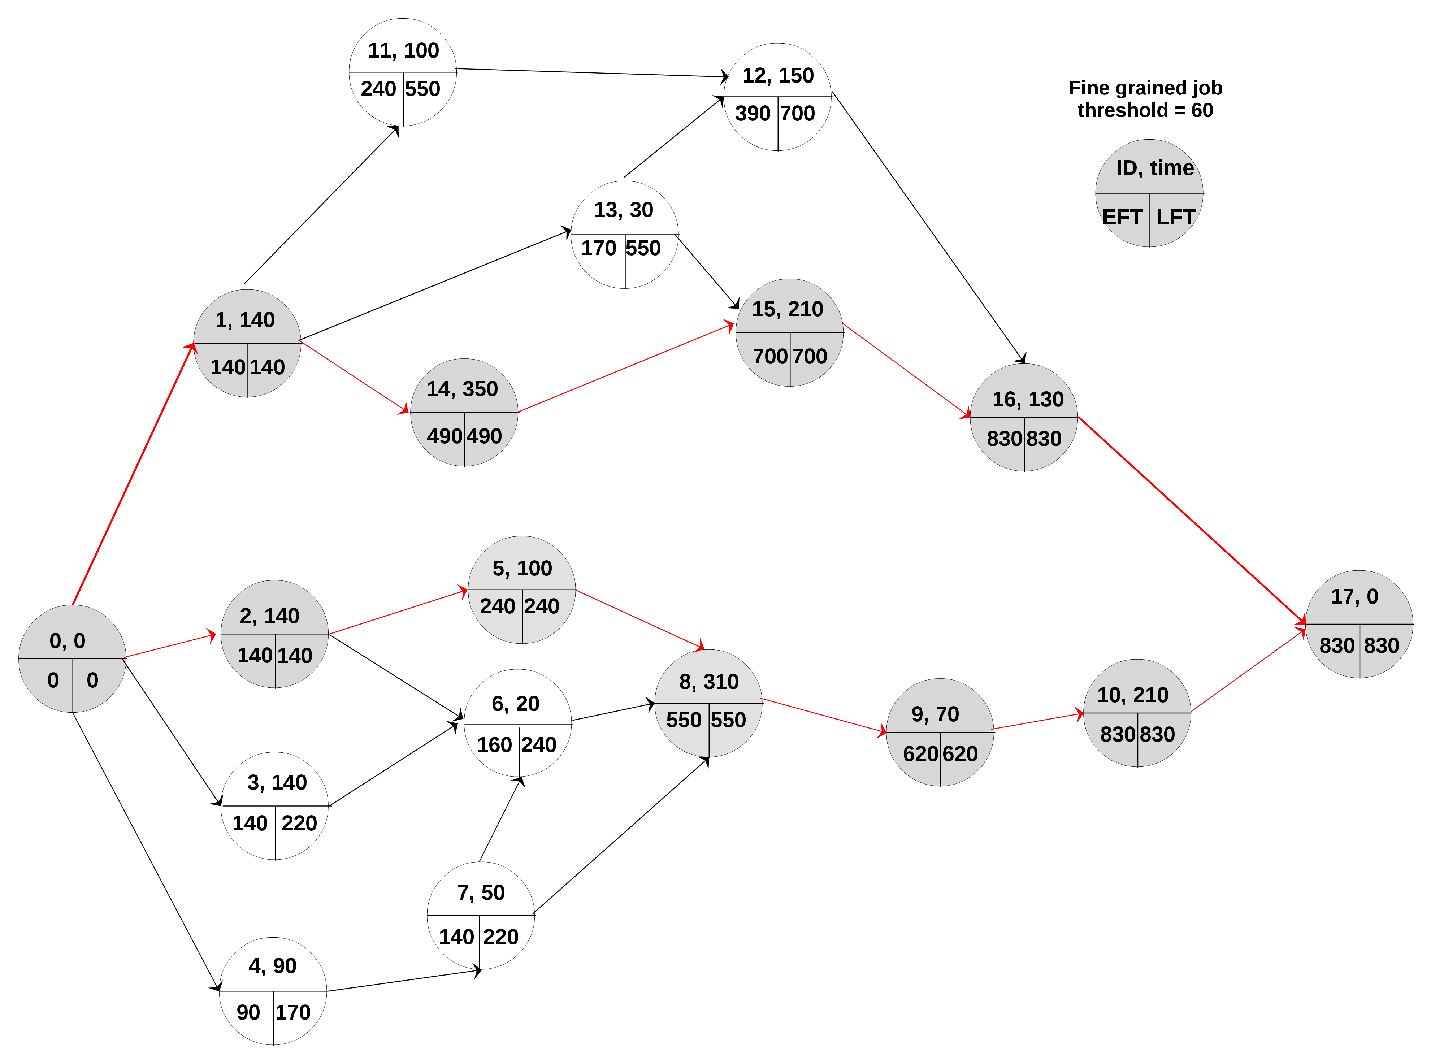
\includegraphics[height=0.77\textheight,width=\textwidth]{imgs/jobgrouping}
    %\caption{Jo}
\end{figure}
\end{frame}

\begin{frame}
\frametitle{Job grouping \hyperlink{jbgrp}{\beamerbutton{algorithm link}}}
\begin{figure}[h]
    \centering
    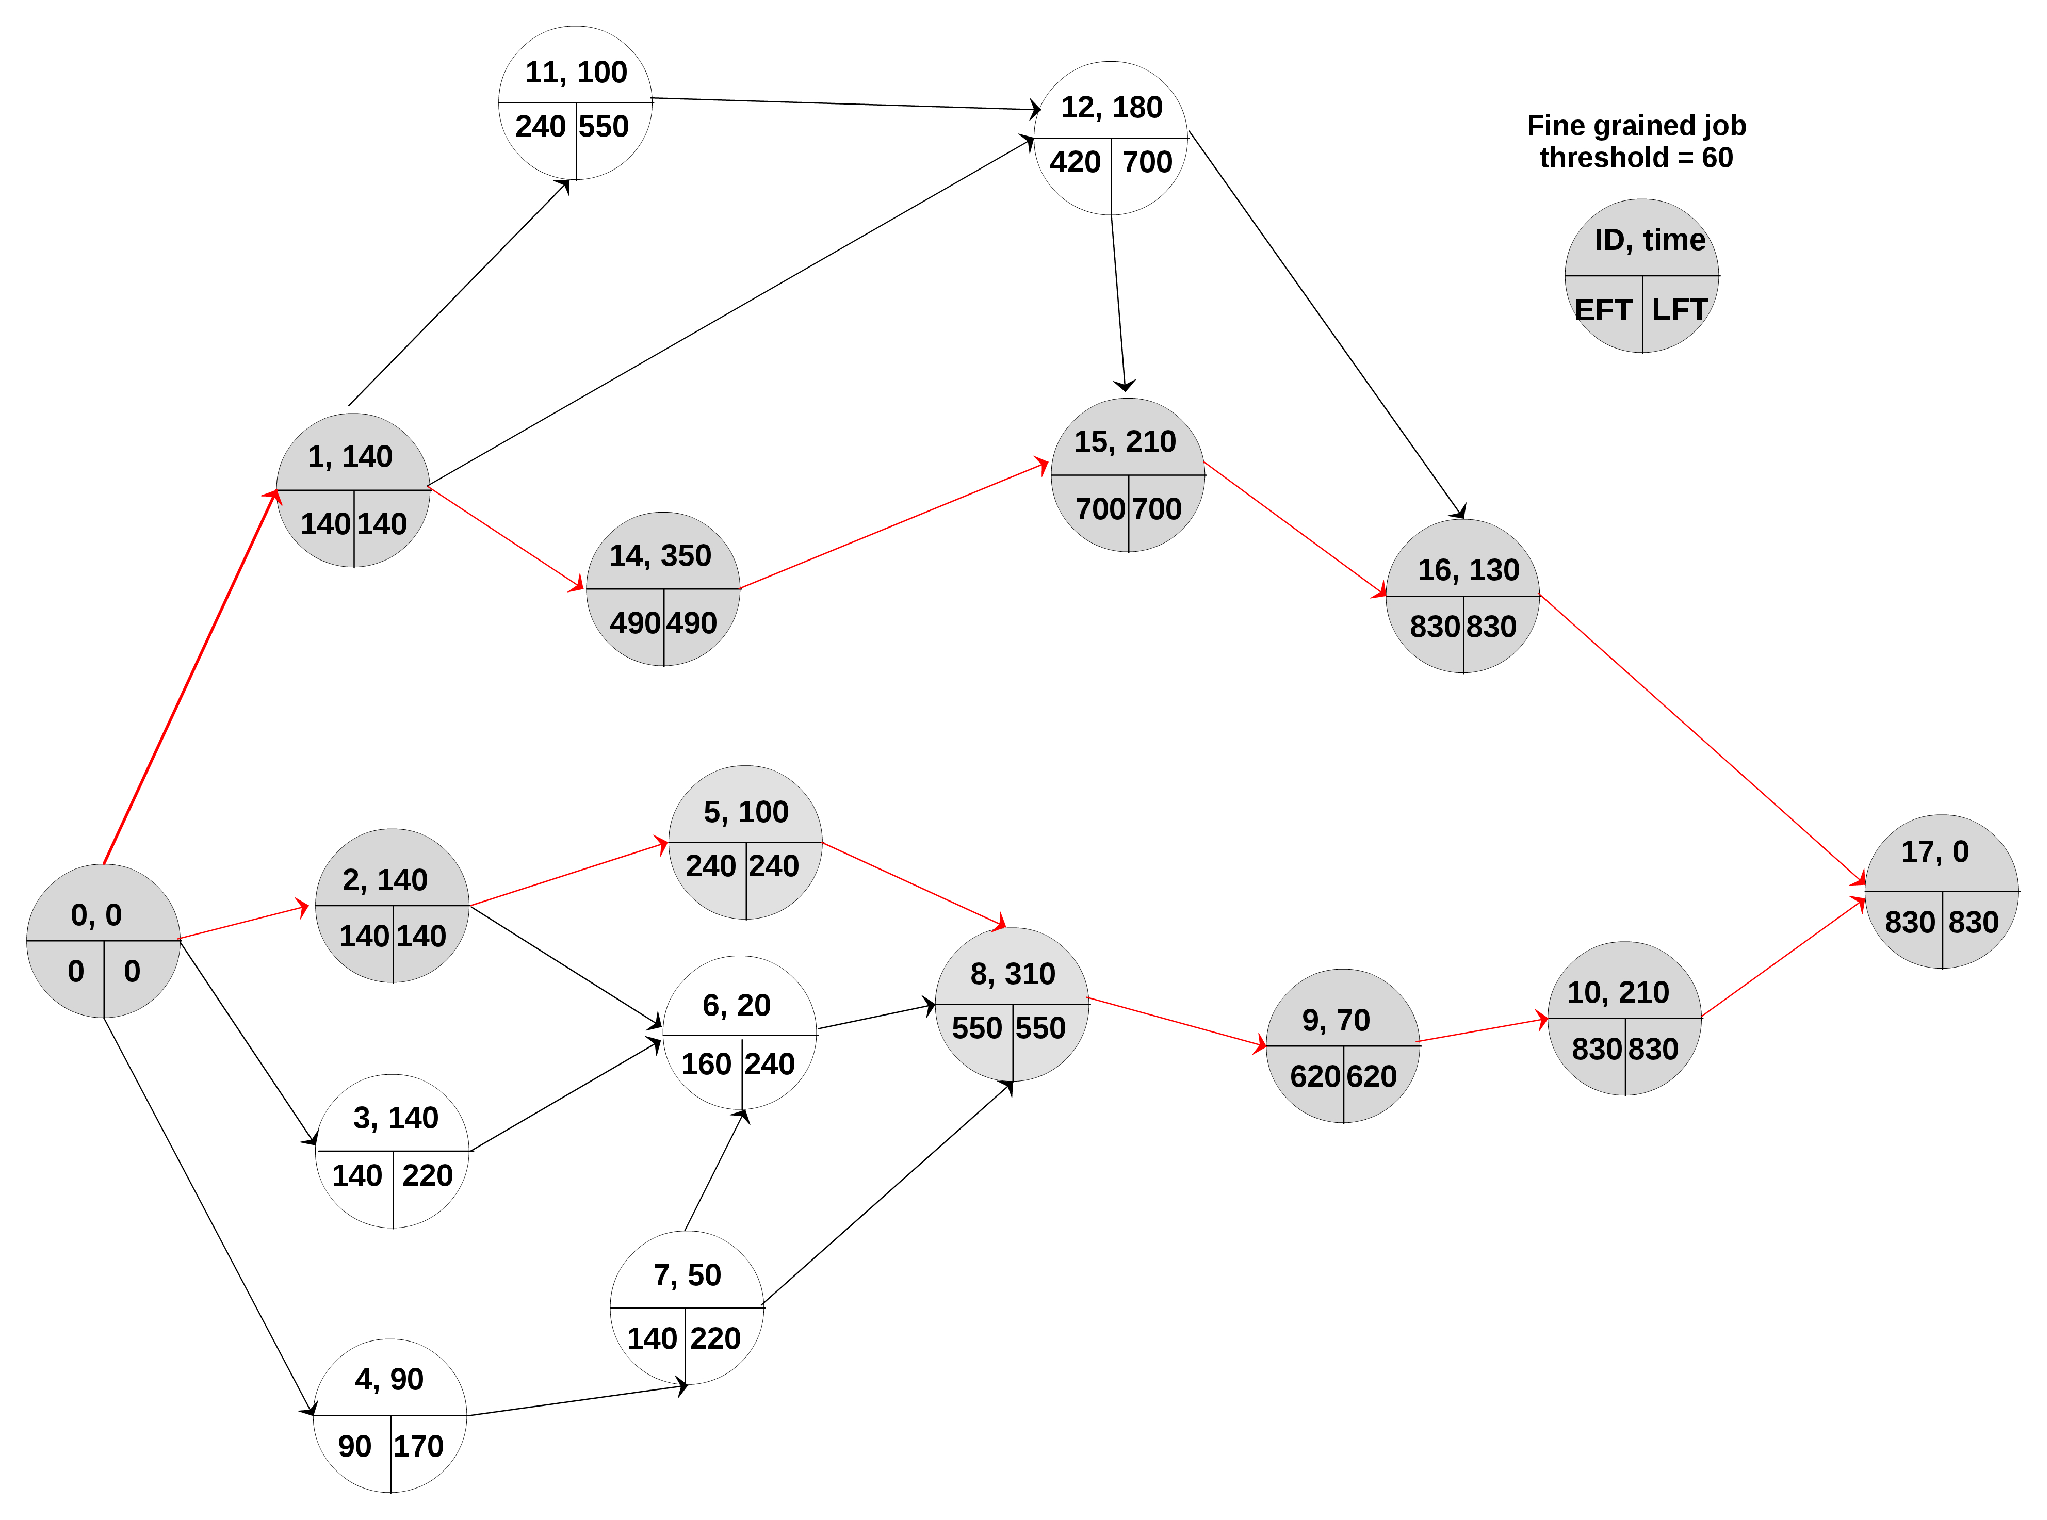
\includegraphics[height=0.77\textheight,width=\textwidth]{imgs/jobgrouping1}
    %\caption{Jo}
\end{figure}
\end{frame}

\begin{frame}
\frametitle{Job grouping \hyperlink{jbgrp}{\beamerbutton{algorithm link}}}
\begin{figure}[h]
    \centering
    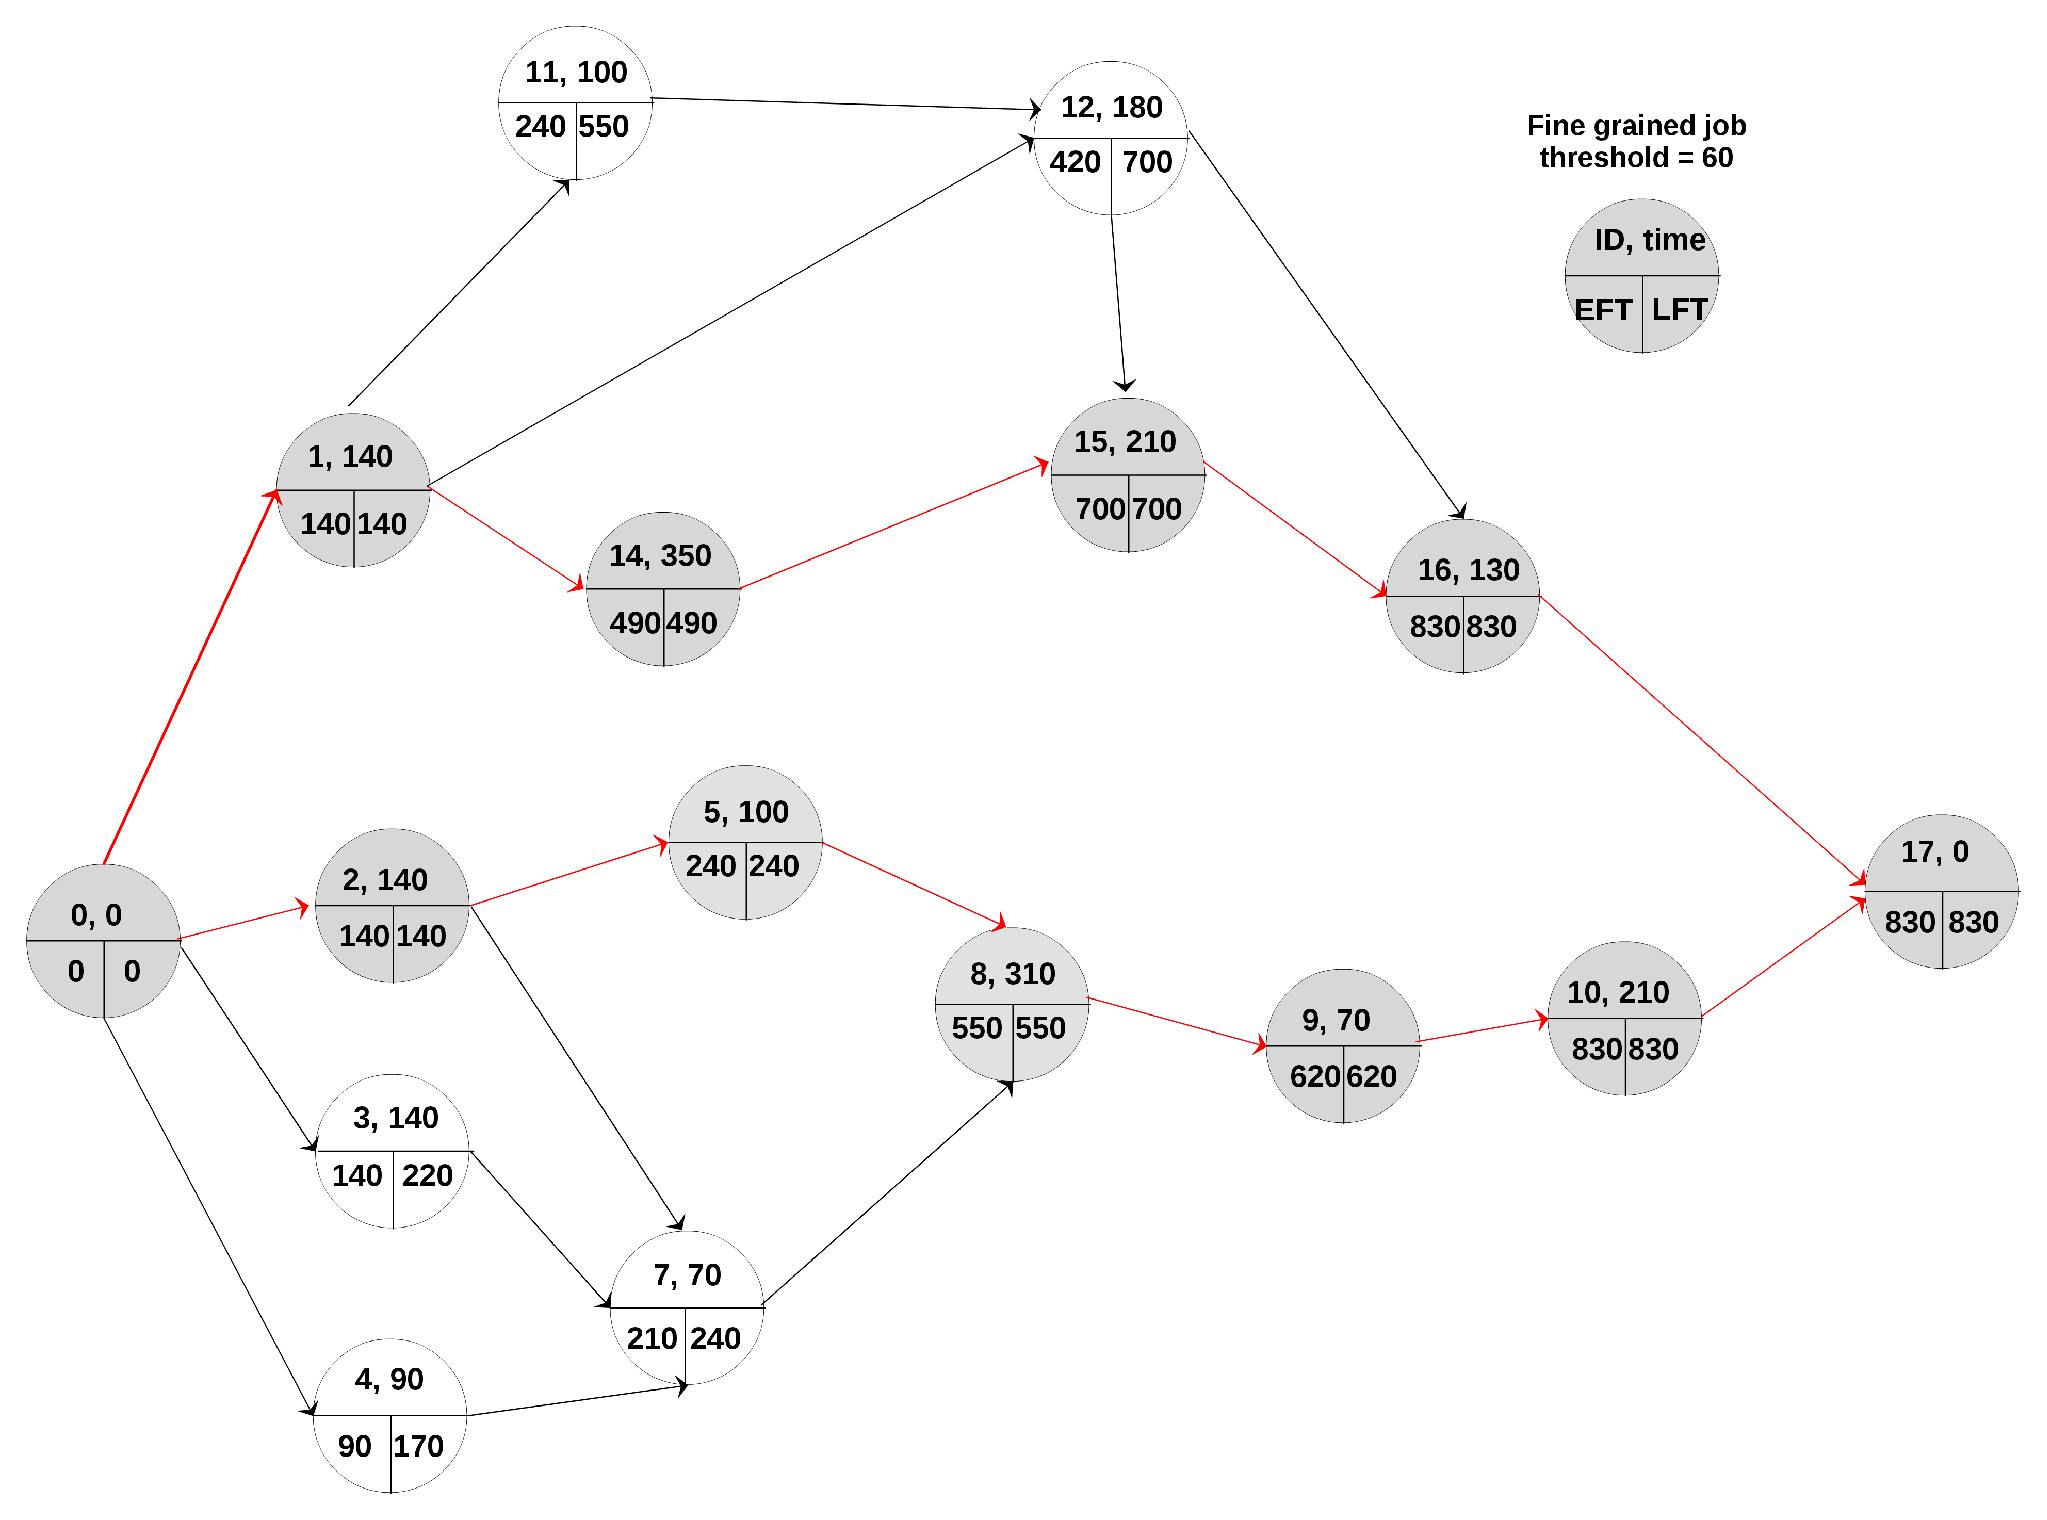
\includegraphics[height=0.77\textheight,width=\textwidth]{imgs/jobgrouping2}
    %\caption{Jo}
\end{figure}
\end{frame}

\begin{frame}
\frametitle{Dynamic scheduler}
\Fontdi
\begin{itemize}
 \item Change in the resource pool can trigger running of MOJS module which can either reschedule the jobs whose resources have left the grid or can request processing of new jobs on addition of one or more resources or both of them. 
 \item Jobs whose predecessors is present in the set of rescheduled jobs are also rescheduled.
 \item Weighted sum approach is applied on multiple objectives to finalize a chromosome as scheduling strategy from first pareto front. 
 \item Some jobs are queued on their respective resource while others are again fed to MOJS module. The number of jobs queued depend on the fitness of the chromosome and time available for the scheduler to re-run and find a better schedule. 
 \item Progress is ensured by setting a minimum number of jobs to be queued on a single run of module.
\end{itemize}
\end{frame}


\comment{
\subsection*{Super-Graph Construction (Continuous)}
\subsection*{Analysis of the Size of Super-Graph}
\begin{frame}
\frametitle{Size (Discrete Case)}
\begin{itemize}
	\item Since the number of ways of drawing any edge is $n \choose 2$, the probability of drawing a contracting edge, therefore, is:
	\begin{align}
		\label{eq8}
		p_c = \sum_{i=1}^k \frac{Y_i(Y_i-1)/2}{n(n-1)/2} 
			> \sum_{i=1}^k \frac{Y_i(Y_i-1)}{n^2}
			> \sum_{i=1}^k \frac{Y_i^2}{n^2} - \frac{1}{n}.
	\end{align}
	\item Since $Y_i^2$ is a convex function with $\sum_{i=1}^k Y_i = n$, using Jensen's inequality, $\sum_{i=1}^k {Y_i^2} \geq \frac{n^2}{k}$.
	\item Putting it back in Eq. \eqref{eq8}, we get:
	%
	\begin{align}
		p_c > \frac{1}{k} - \frac{1}{n} \approx \frac{1}{k}. 
	\end{align}
\end{itemize}
\end{frame}

\subsection*{Reduction of the Super-graph}
\begin{frame}[label=main6]
\Fontvi
\frametitle{Reduction of the Super-graph}
\begin{block}{Lemma 6}
	Suppose $X_1^2$ and $X^2_2$ represent the $X^2$ values of super-vertices
	$v_{s_1}$ and $v_{s_2}$ in $G_s$. The $X^2$ value of the new super-vertex
	$X^2_{c}$ formed by clubbing $v_{s_1}$ and $v_{s_2}$ is upper bounded by
	$X_1^2 + X^2_2$, and trivially lower bounded by $0$ \hyperlink{supplement8}{\beamerbutton{more}}
\end{block}
\begin{itemize}
	\item In each iteration of the algorithm, the edge connecting the two vertices that have the least sum of $X^2$ values is contracted, thereby reducing the number of super-vertices by $1$ in every iteration.
	\item The corresponding vertices are merged and all their neighboring vertices become neighbors of this new vertex.  As a result, in the final solution, the \ms or \ts either contains both these vertices or none of them.  
	\item This may introduce non-optimality as only one of them may have been part of the optimal solution.
\end{itemize}
\end{frame}
}

\section[Experimentation]{Experimentation}
\subsection*{Implemented system model}
\begin{frame}
 \frametitle{Implemented system model}
\begin{figure}[t]
    \centering
    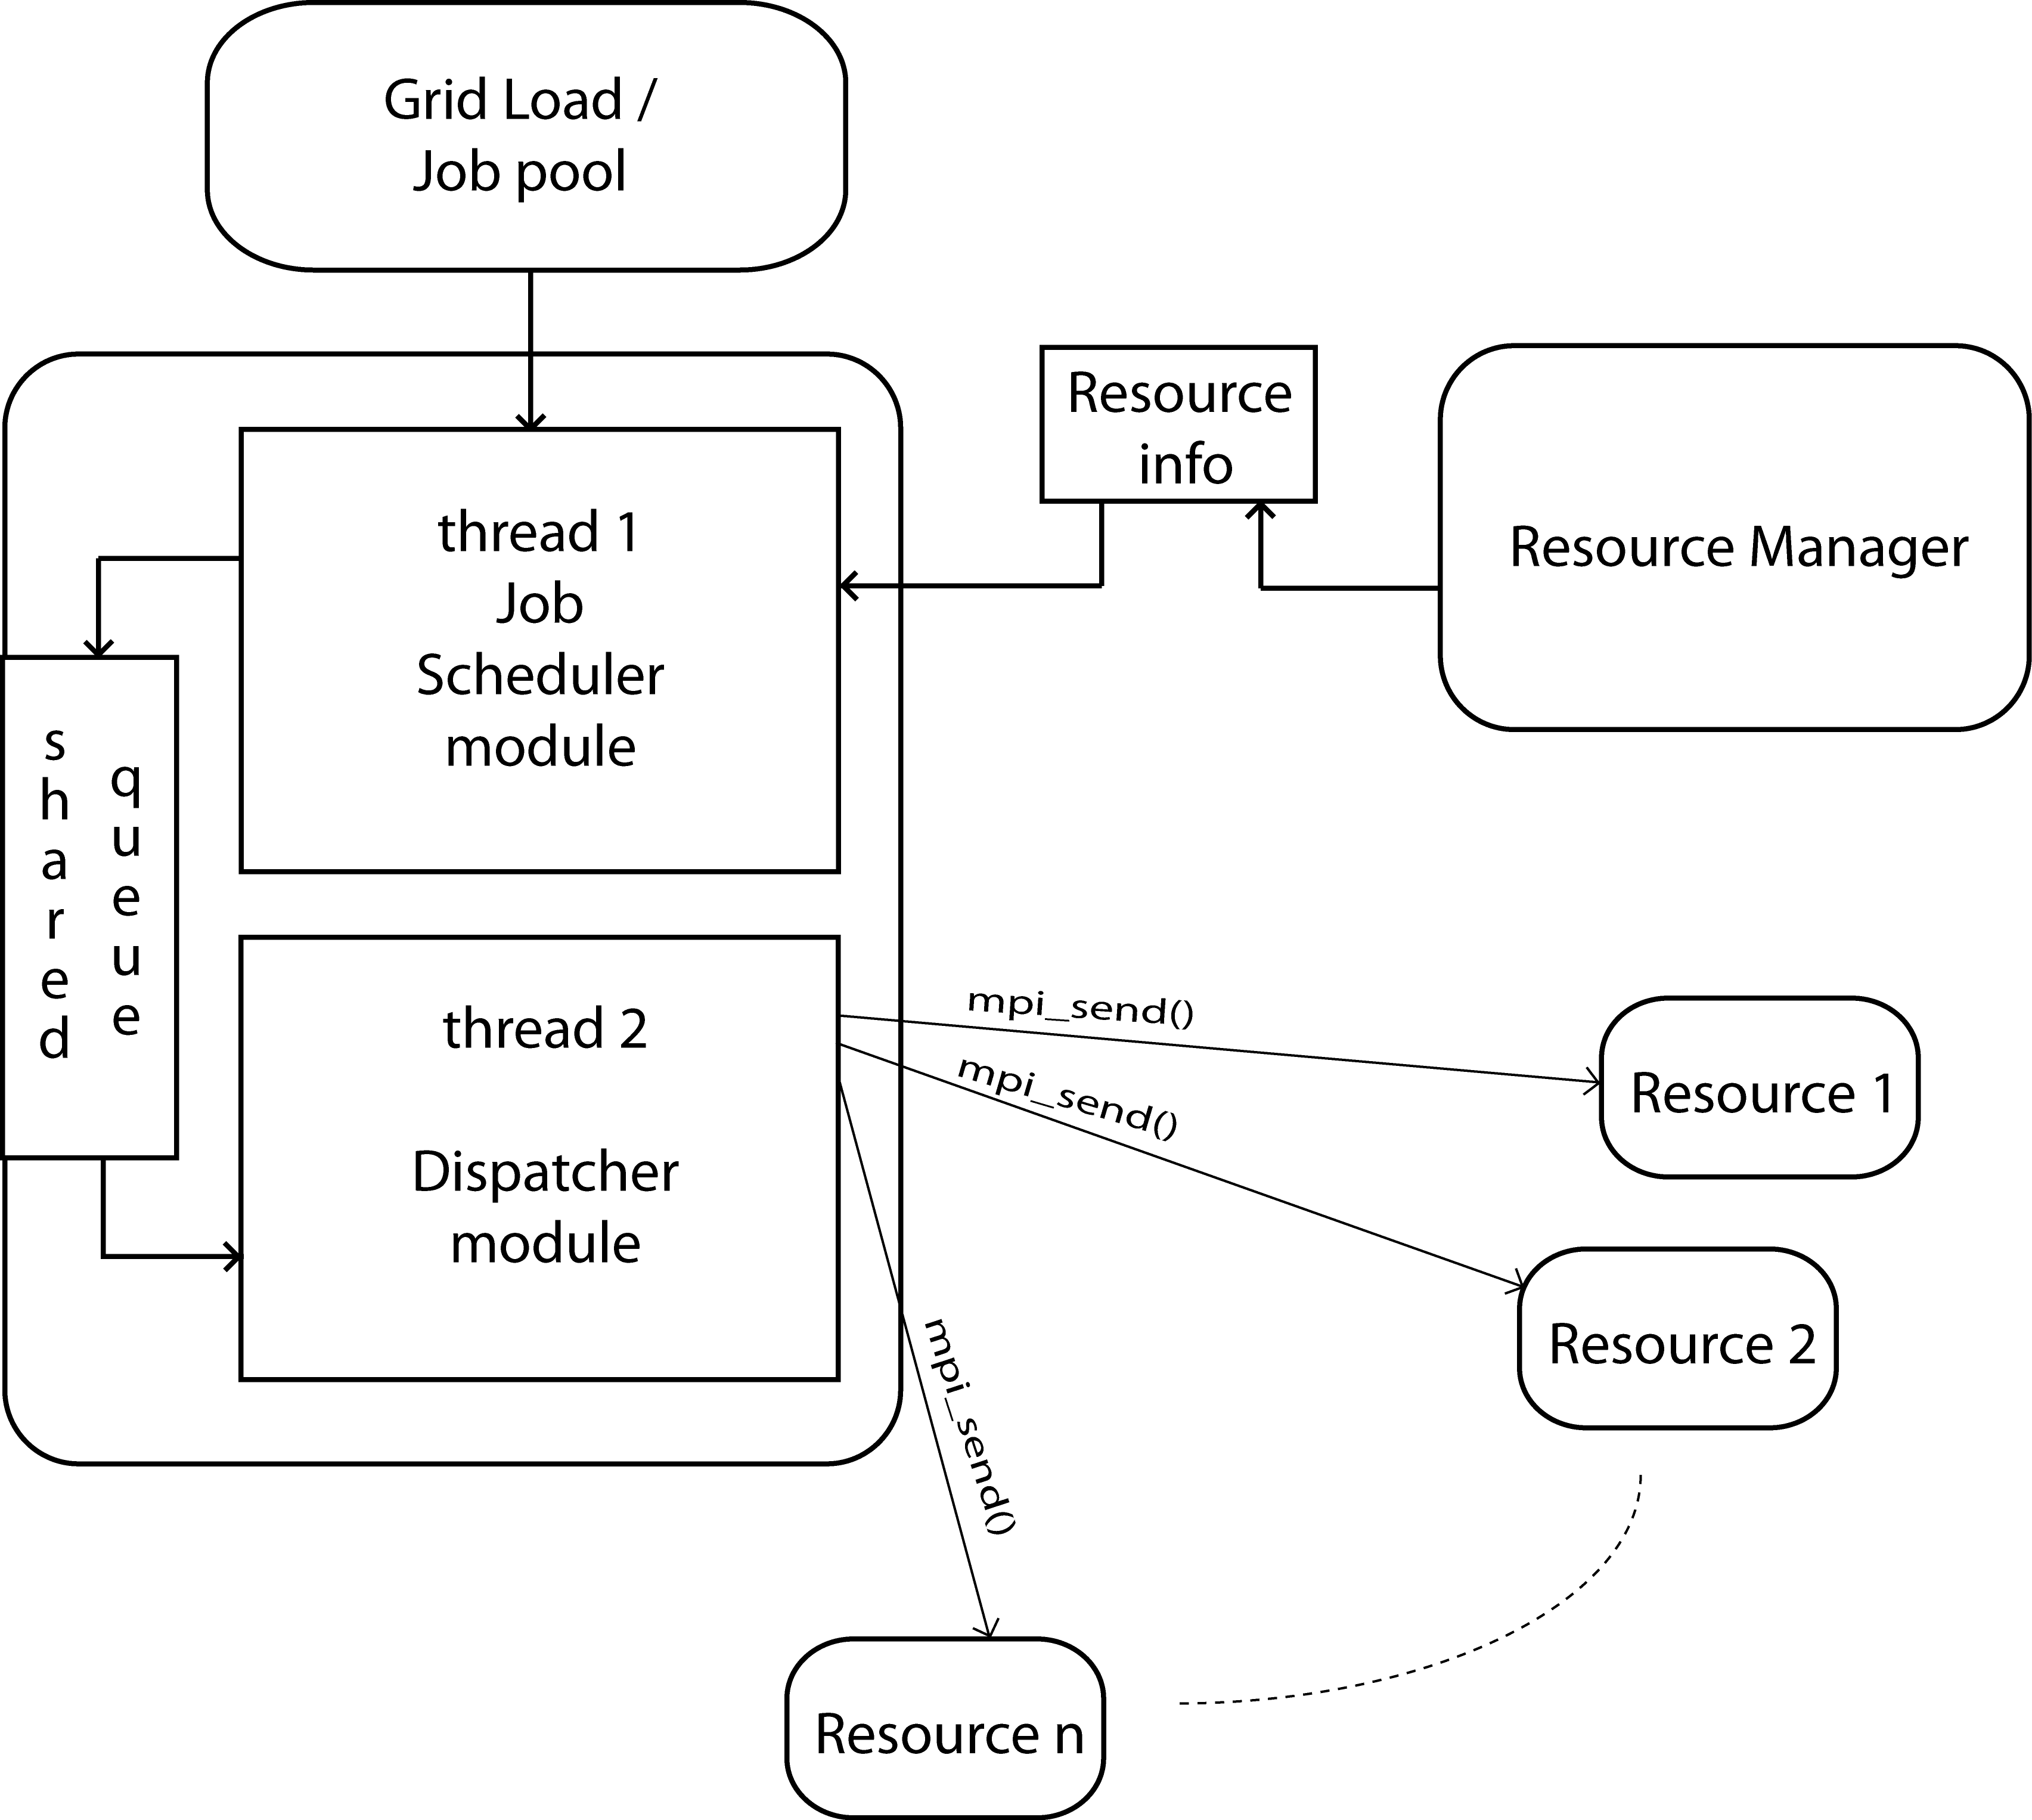
\includegraphics[height=0.82\textheight]{imgs/implement}
    %\caption{Implemented System model}
	\label{fig:Systemmodel}
\end{figure}
\end{frame}


\comment{
\begin{frame}
 \frametitle{Implemented system model}
\begin{table}[ht]
\caption{User job queue}
\scalebox{0.7}{
    \begin{tabular}{|c|r|c|c|c|c|}
    \hline \hline
    $JOB\_ID$ & $JOB\_SIZE$ & $TIME\_LIMIT$ & $JOB\_COST$ & $PRED\_ID$ & $JOB\_TYPE$ \\ 
     & in MI/MB & in seconds & in \$ &  &  \\ \hline
    $\vdots$ & $\vdots$ & $\vdots$   & $\vdots$ & $\vdots$	     & $\vdots$  \\
    42     & 24,000 MI  & 63.0  & 5.41 & 29                 & 0        \\
    43     & 130,000 MI  & 107.0 & 4.86 & -1                 & 0        \\
    44     & 10,500 MI  & 106.0 & 5.99 & 24                 & 0        \\ 
    47     & 530.0 MB  & 150.0 & 5.04 & 29   	       & 1	\\
    48     & 240,200 MI  & 133.0 & 5.40 & 31   	       & 0        \\
    $\vdots$ & $\vdots$ & $\vdots$   & $\vdots$ & $\vdots$	     & $\vdots$  \\ \hline
    \end{tabular}
}
\label{jobmodel}
\end{table}
\begin{table}[ht]
\caption{Resource configuration}
\scalebox{0.7}{
    \begin{tabular}{|c|r|c|c|r|}
    \hline \hline
    $RESOURCE\_ID$ & $RES\_COST$ & $RES\_TYPE$ & $RES\_ENERGY$  & $RES\_CAP$ \\ 
     & in \$ &  & \emph{normalized}  & {\small in MIPS/MBPS} \\ \hline \hline
    $\vdots$ & $\vdots$ & $\vdots$   & $\vdots$ & $\vdots$  \\
    4 & 0.13 & 0 & 0.943 & 9,726 MIPS   \\
    5 & 0.14 & 0 & 1.000 & 29,621 MIPS   \\
    6 & 0.13 & 0 & 0.577 & 13,539 MIPS \\
    7 & 0.11 & 1 & 0.894 & 30.0 MBPS     \\
    $\vdots$ & $\vdots$ & $\vdots$   & $\vdots$ & $\vdots$  \\ \hline
    \end{tabular}
}
\label{resconf}
\end{table}
\end{frame}
}

\subsection*{Data Sets}
\begin{frame}
\frametitle{Data sets}
\Fontdi
\begin{itemize}
 \item Standard grid workload from Grid Workload Archive have been used in this experiments \cite{gridload}.
  \begin{itemize}
  \item SHARCNET \& DAS-2 are the two traces that have been processed.
  \item Traces shows that execution time of jobs ranges from 1 to 20000 time units in DAS-2, and 1 to 100000 time units in SHARCNET.
  \end{itemize}
  \begin{table}[ht]
%  \caption{Gridlet configuration}
  \centering
  \scalebox{0.7}{
    \begin{tabular}{|c|c|c|c|}
    \hline \hline
    Workload\_id & Trace        & Precedence constraint & Resource constraint \\ \hline
    1 	         & DAS-2    & \xmark                 & \xmark   \\
    2 	         & SHARCNET & \xmark                 & \xmark   \\
    3 	         & DAS-2    & \xmark                 & \cmark   \\
    4 	         & SHARCNET & \xmark                 & \cmark   \\
    5	         & DAS-2    & \cmark                 & \xmark   \\
    6	         & SHARCNET & \cmark                 & \xmark   \\
    7	         & DAS-2    & \cmark                 & \cmark   \\
    8 	         & SHARCNET & \cmark                 & \cmark   \\ \hline \hline
    \end{tabular}
  }
  \label{tab:gridlet}
  \end{table}
\end{itemize}
\end{frame}

\subsection*{Results}
\begin{frame}
\frametitle{1. Experiment on independent jobs}
\begin{figure}[!ht]
    \centering
    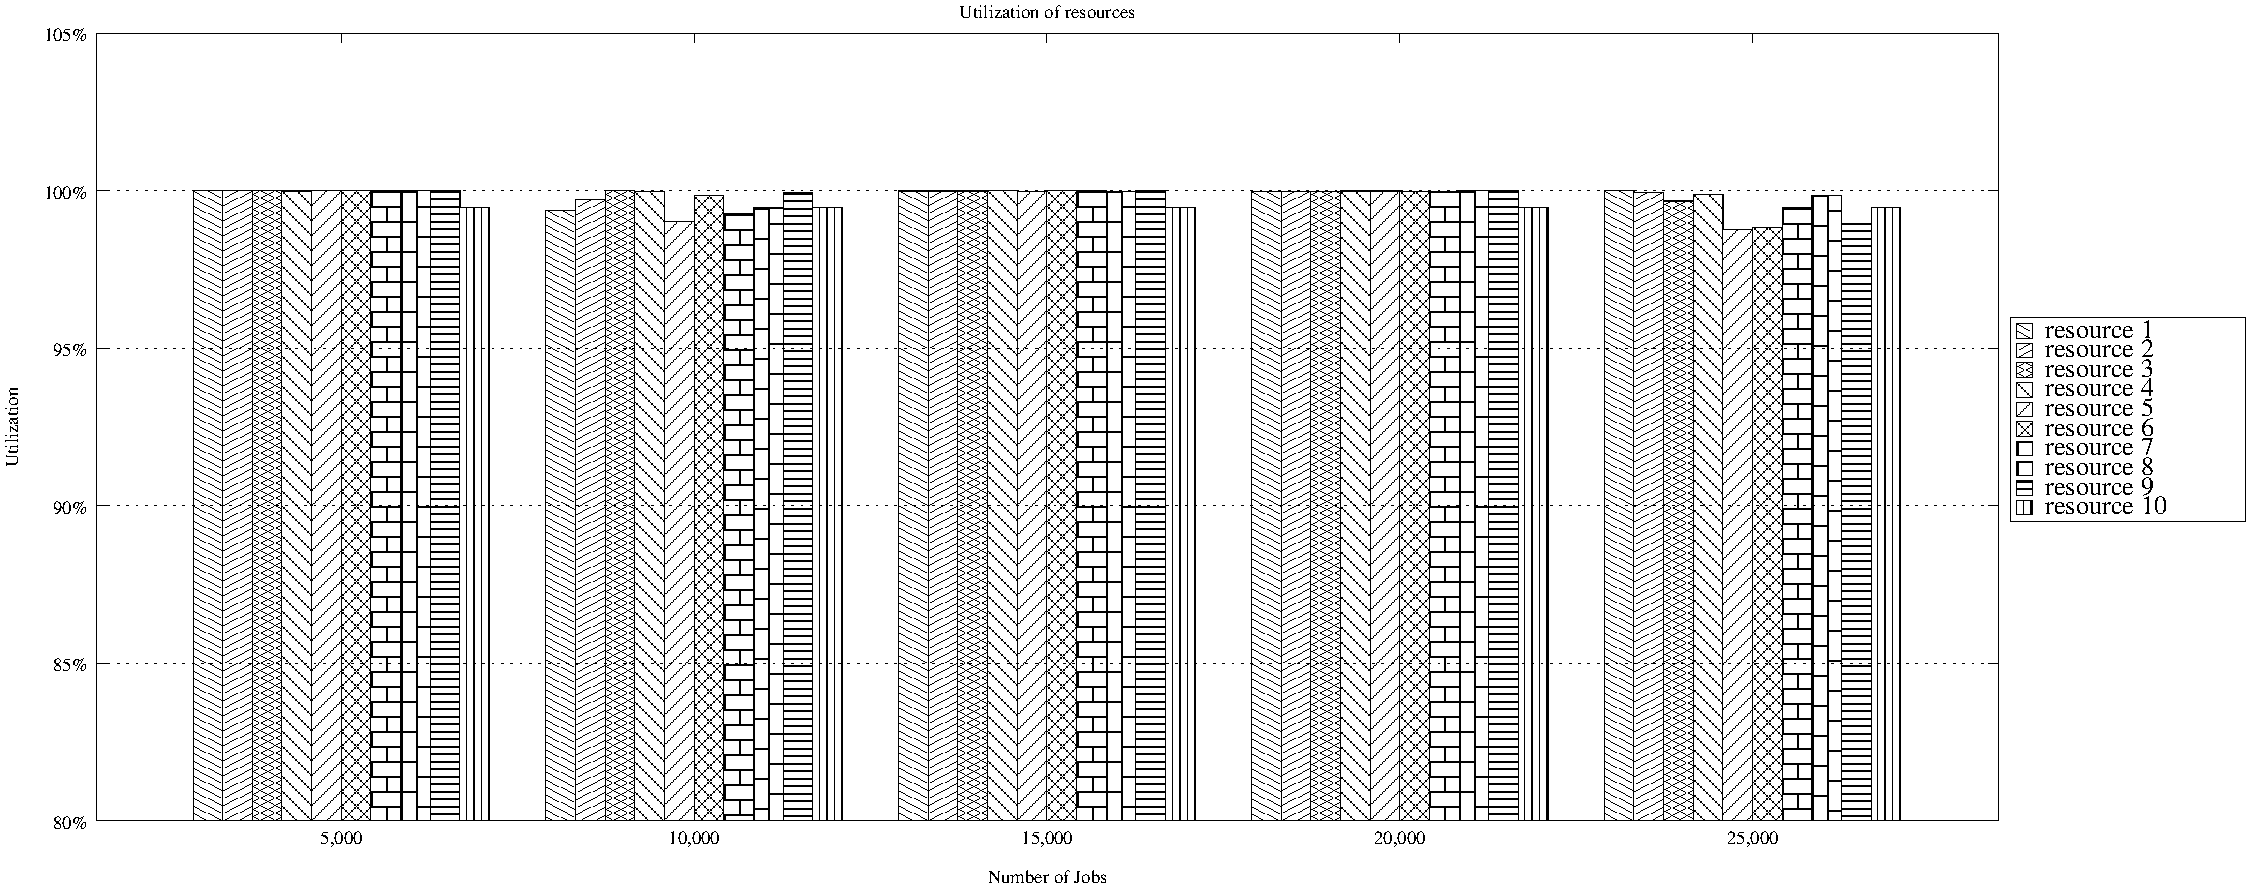
\includegraphics[width=1.02\textwidth,keepaspectratio]{imgs/10res_SHARCNET}
    \caption{Evaluation of makespan and utilization on 10 resources on workload 2}
    \label{fig:10res}
\end{figure}
\end{frame}

\begin{frame}
 \frametitle{1. Experiment on independent jobs}
\begin{figure}[h]
    \centering
    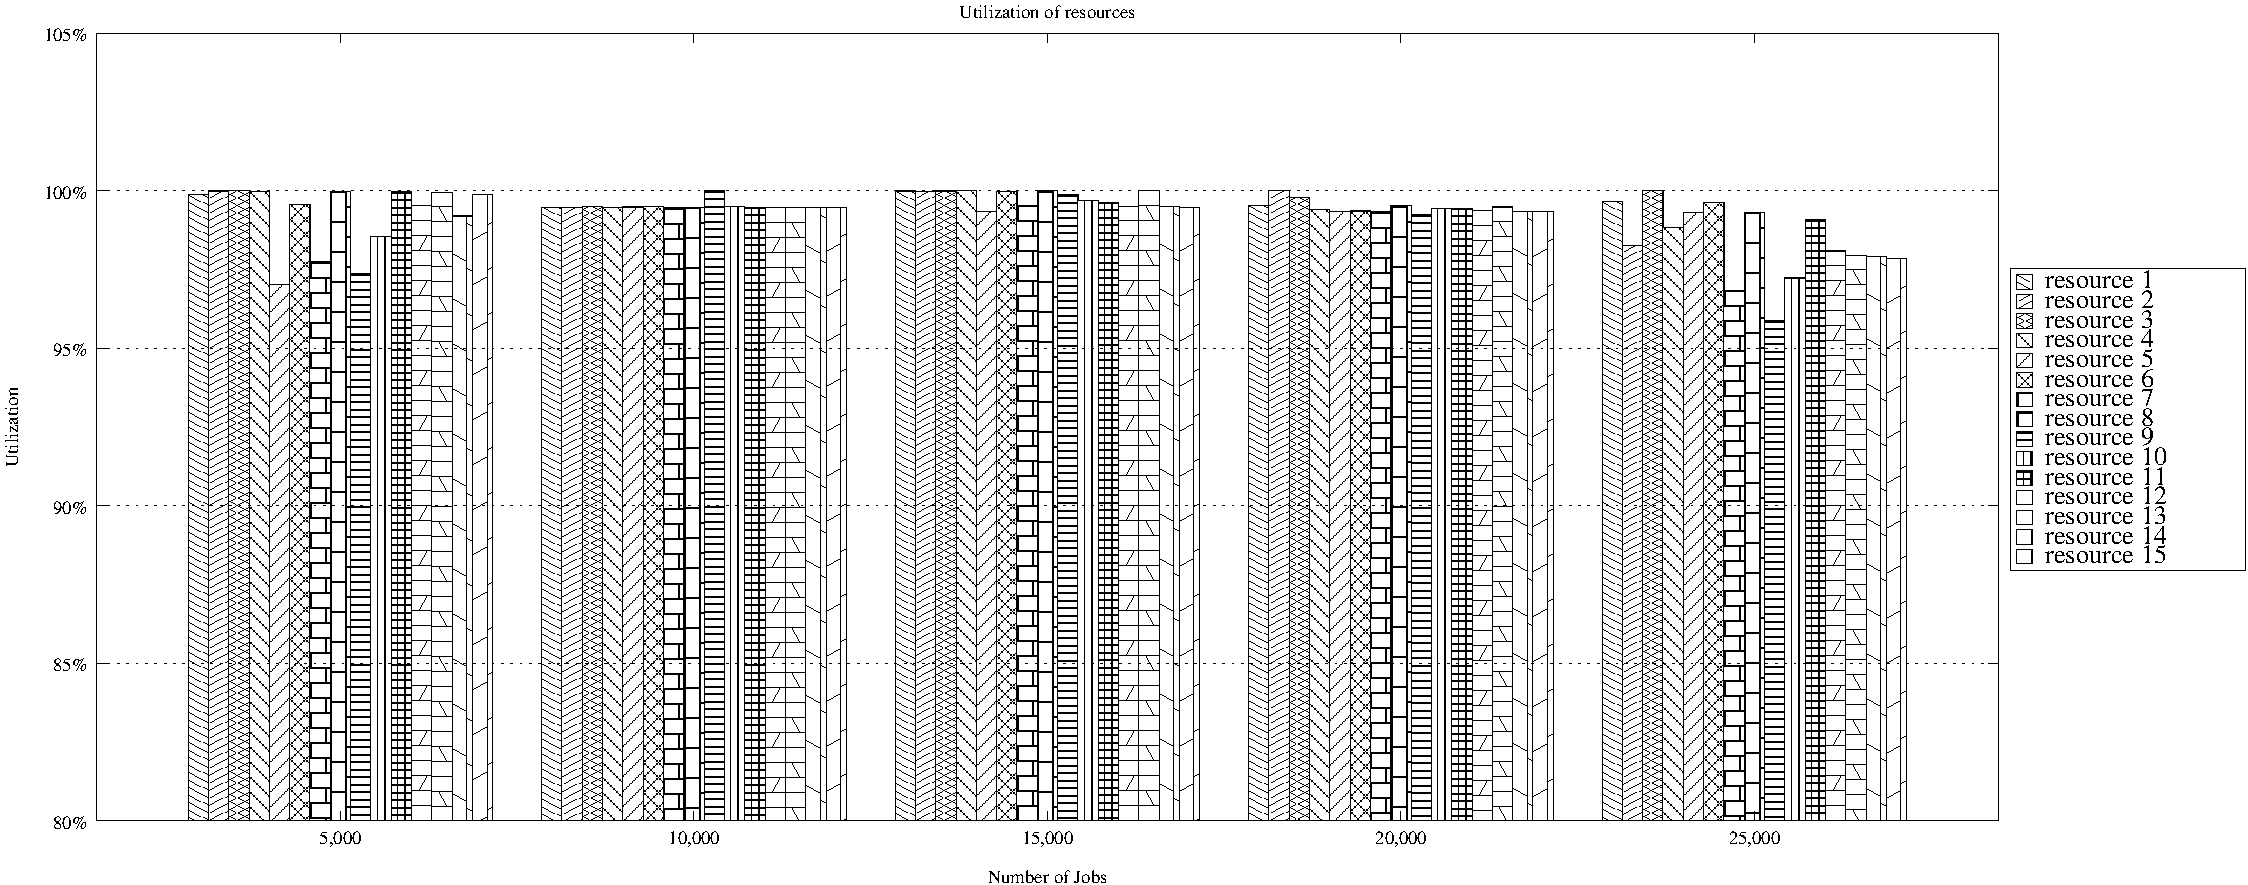
\includegraphics[width=1.02\textwidth,keepaspectratio]{imgs/15res_SHARCNET}
    \caption{Evaluation of makespan and utilization on 15 resources on workload 1}
    \label{fig:15res}
\end{figure}
\end{frame}

\begin{frame}
 \frametitle{1. Experiment on independent jobs}
\begin{figure}[h]
    \centering
    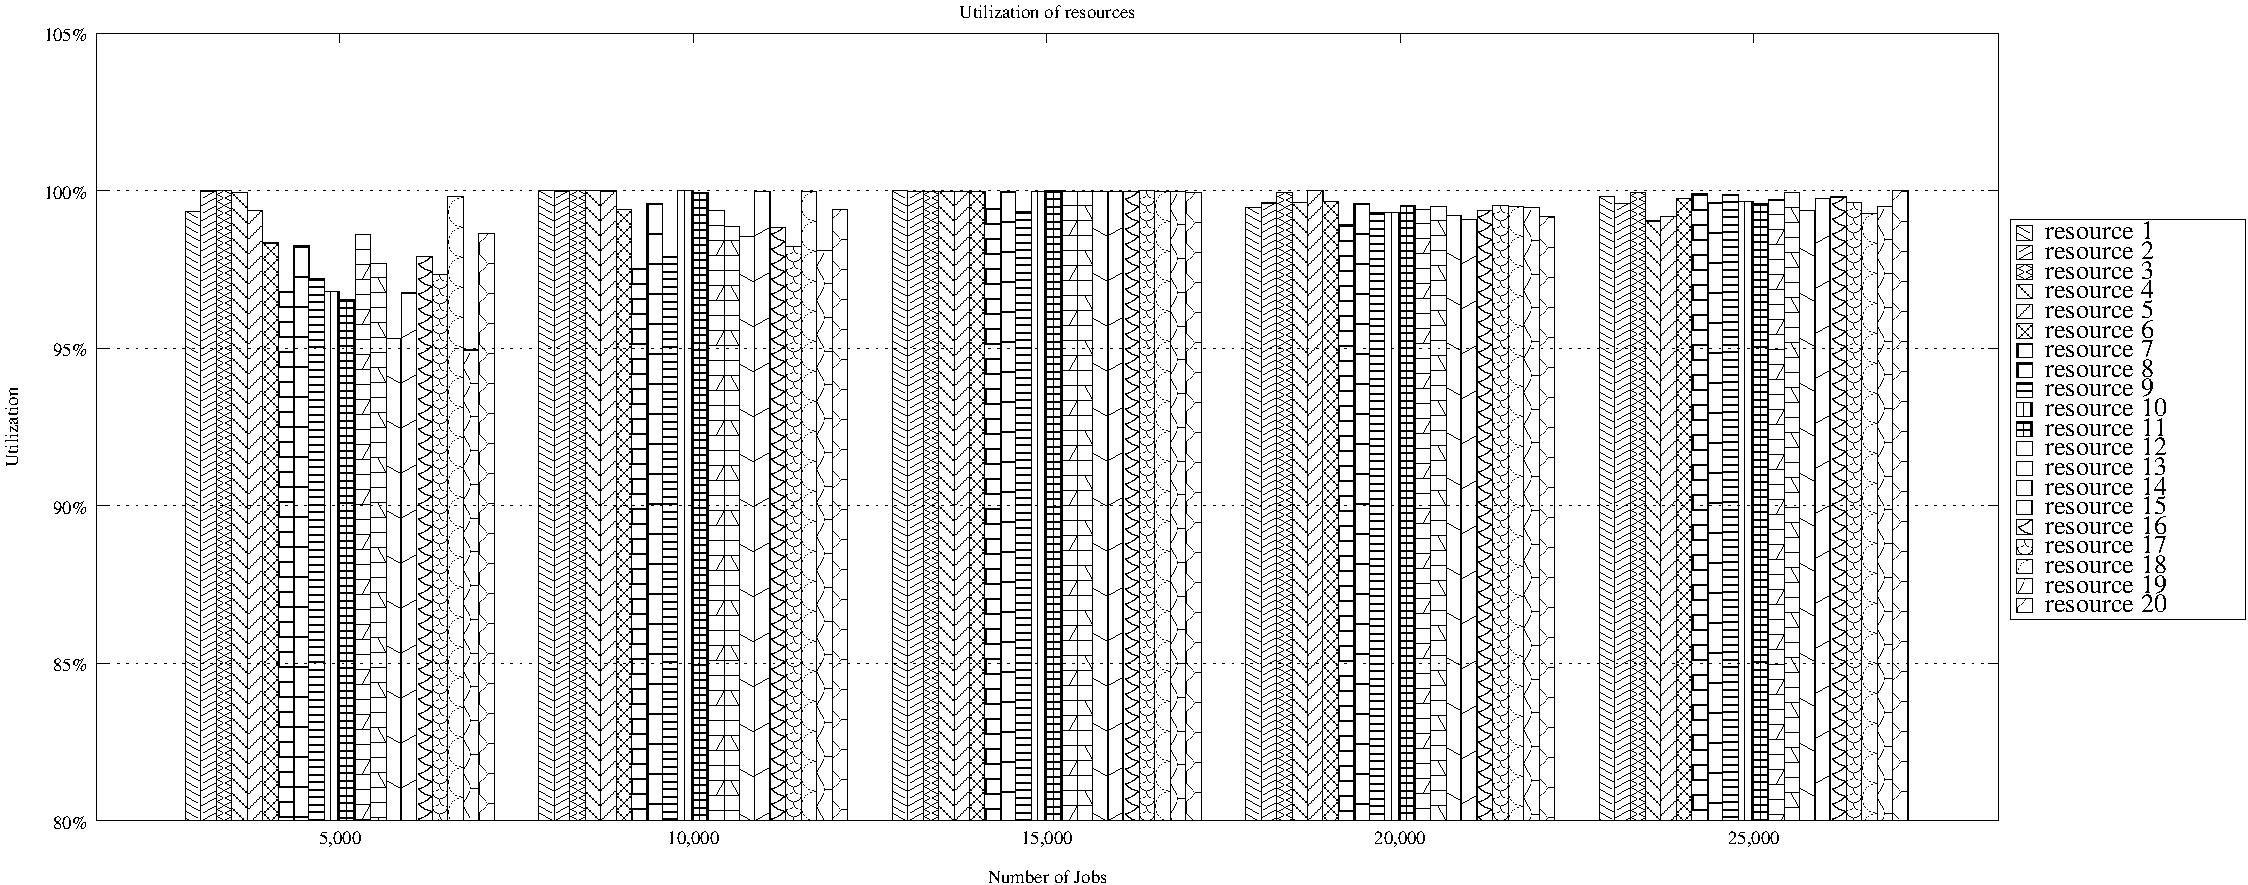
\includegraphics[width=1.02\textwidth,keepaspectratio]{imgs/20res_SHARCNET}
    \caption{Evaluation of makespan and utilization on 20 resources on workload 1}
    \label{fig:20res}
\end{figure}
\end{frame}

\begin{frame}
 \frametitle{1. Experiment on independent jobs}
\begin{figure}[!ht]
     \centering
    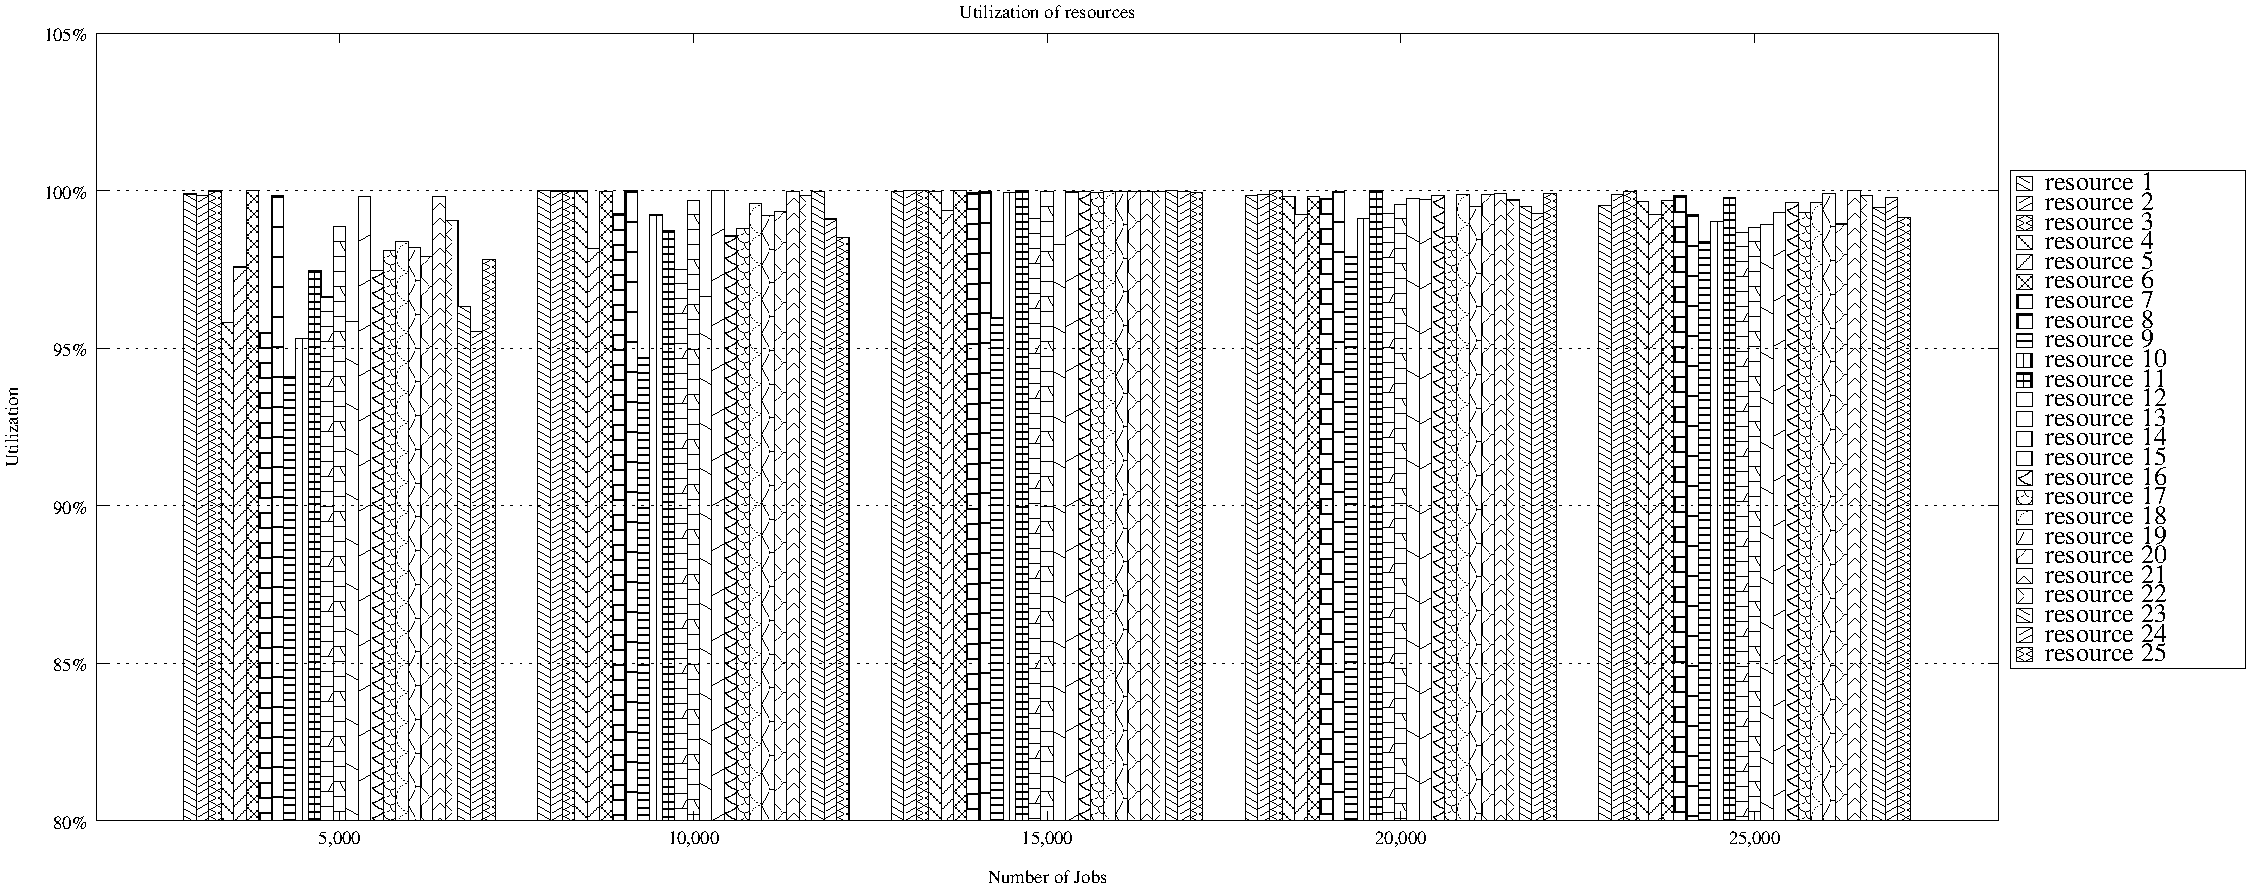
\includegraphics[width=1.02\textwidth,keepaspectratio]{imgs/25res_SHARCNET}
    \caption{Evaluation of makespan and utilization on 25 resources on workload 2}
    \label{fig:25res}
\end{figure}
\end{frame}

\begin{frame}
\frametitle{2. Experiment on trade off between energy consumption and performance}
 \begin{table}[ht]
\caption{Resource configuration for experiment on workload 1 and 2 }
\centering
\scalebox{0.7}{
    \begin{tabular}{|l|l|c|c|c|}
    \hline \hline
    Machine & Frequency & Watts & MIPS/core & Resource\_id \\ \hline
Pentium 4 Extreme Edition 	&	3.2 GHz 	&	92.1	& 	9,726	 & 1,2 \\ \hline
Intel Core 2  X6800 (Dual core) 	&	2.93 GHz	&	75	&	13,539	& 3,4 \\ \hline
Intel Core 2  QX6700 (Quad core) 	&	2.66 GHz 	&	95	&	12,290 & 5,6	 \\ \hline
Intel Core i7 920 (Quad core) 	&	2.667 GHz 	&	130	&	20,575	 & 7,8 \\ \hline
Intel Core i7 3960X (Hex core) 	&	3.3 GHz	&	130	&	29,621	& 9,10  \\ \hline
Core i7-2600 	&	3.4 GHz	&	95	&	32,075	 & 11, 12 \\ \hline
\end{tabular}
}
\end{table}
\end{frame}

\begin{frame}
 \frametitle{2. Experiment on trade off between energy consumption and performance}
\begin{figure}[h]
\centering
    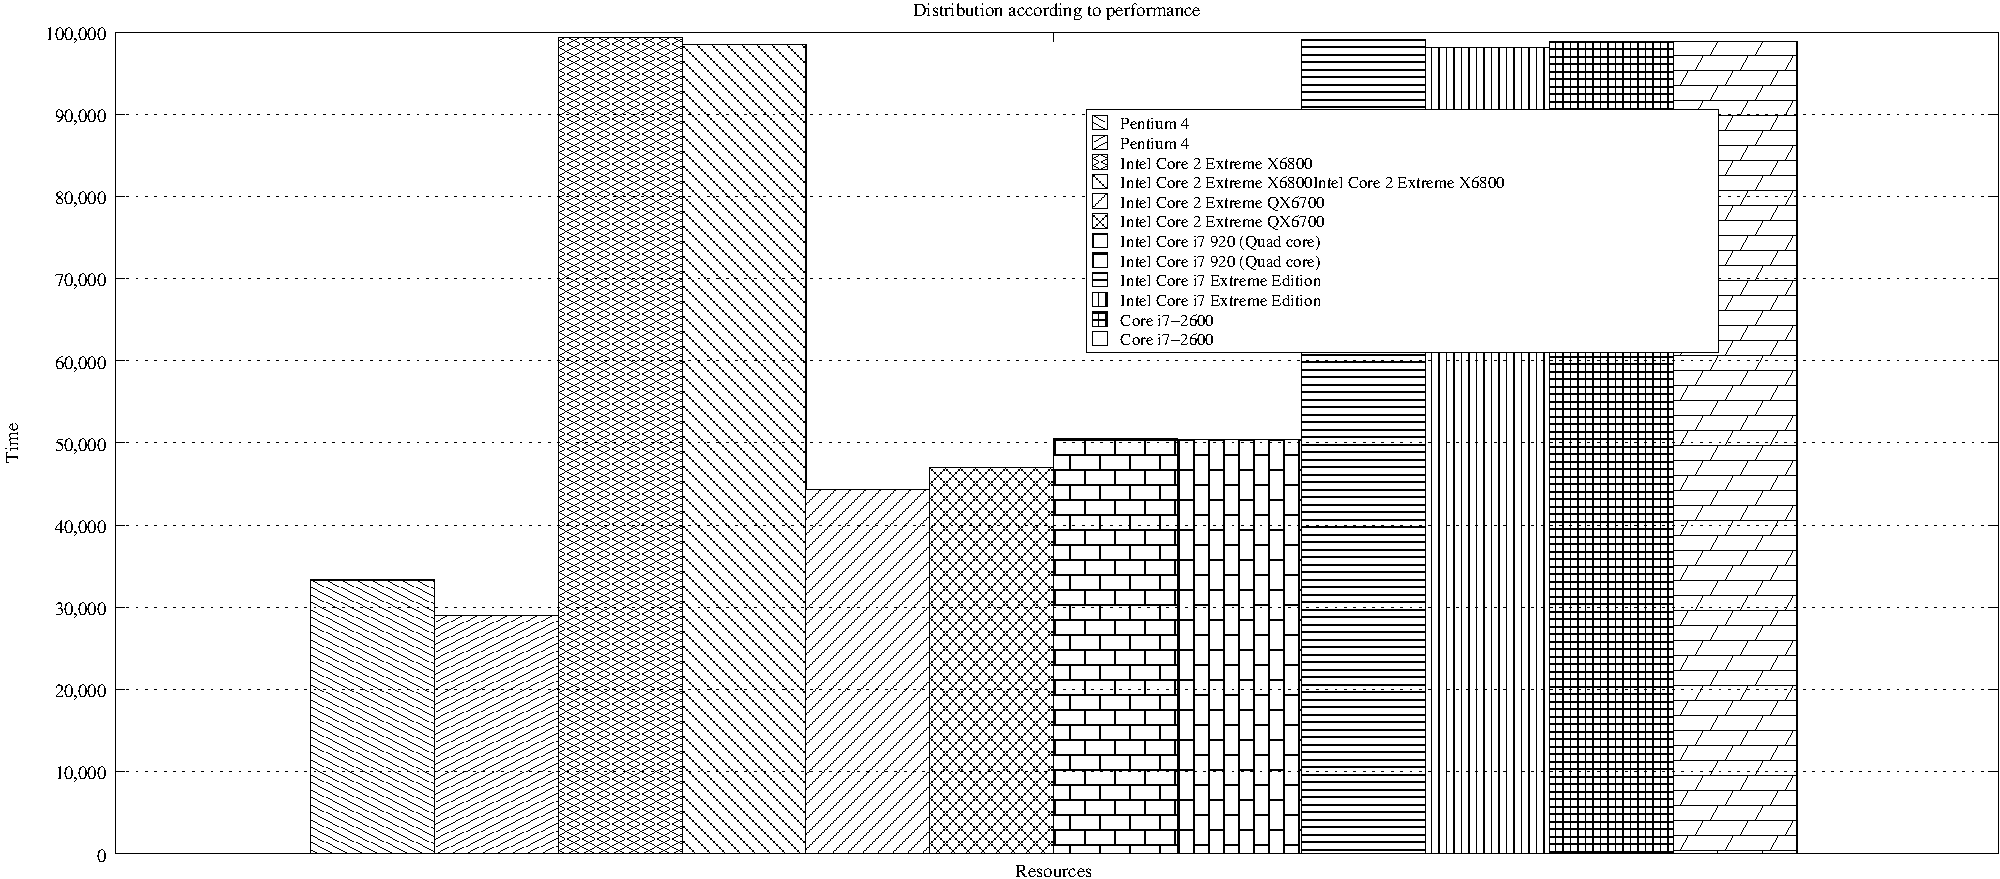
\includegraphics[width=\textwidth]{imgs/case2SHARCNET}
    \caption{Workload 2 (SHARCNET)}
\end{figure}
\end{frame}

\begin{frame}
  \frametitle{2. Experiment on trade off between energy consumption and performance}
\begin{figure}[h]
\centering
    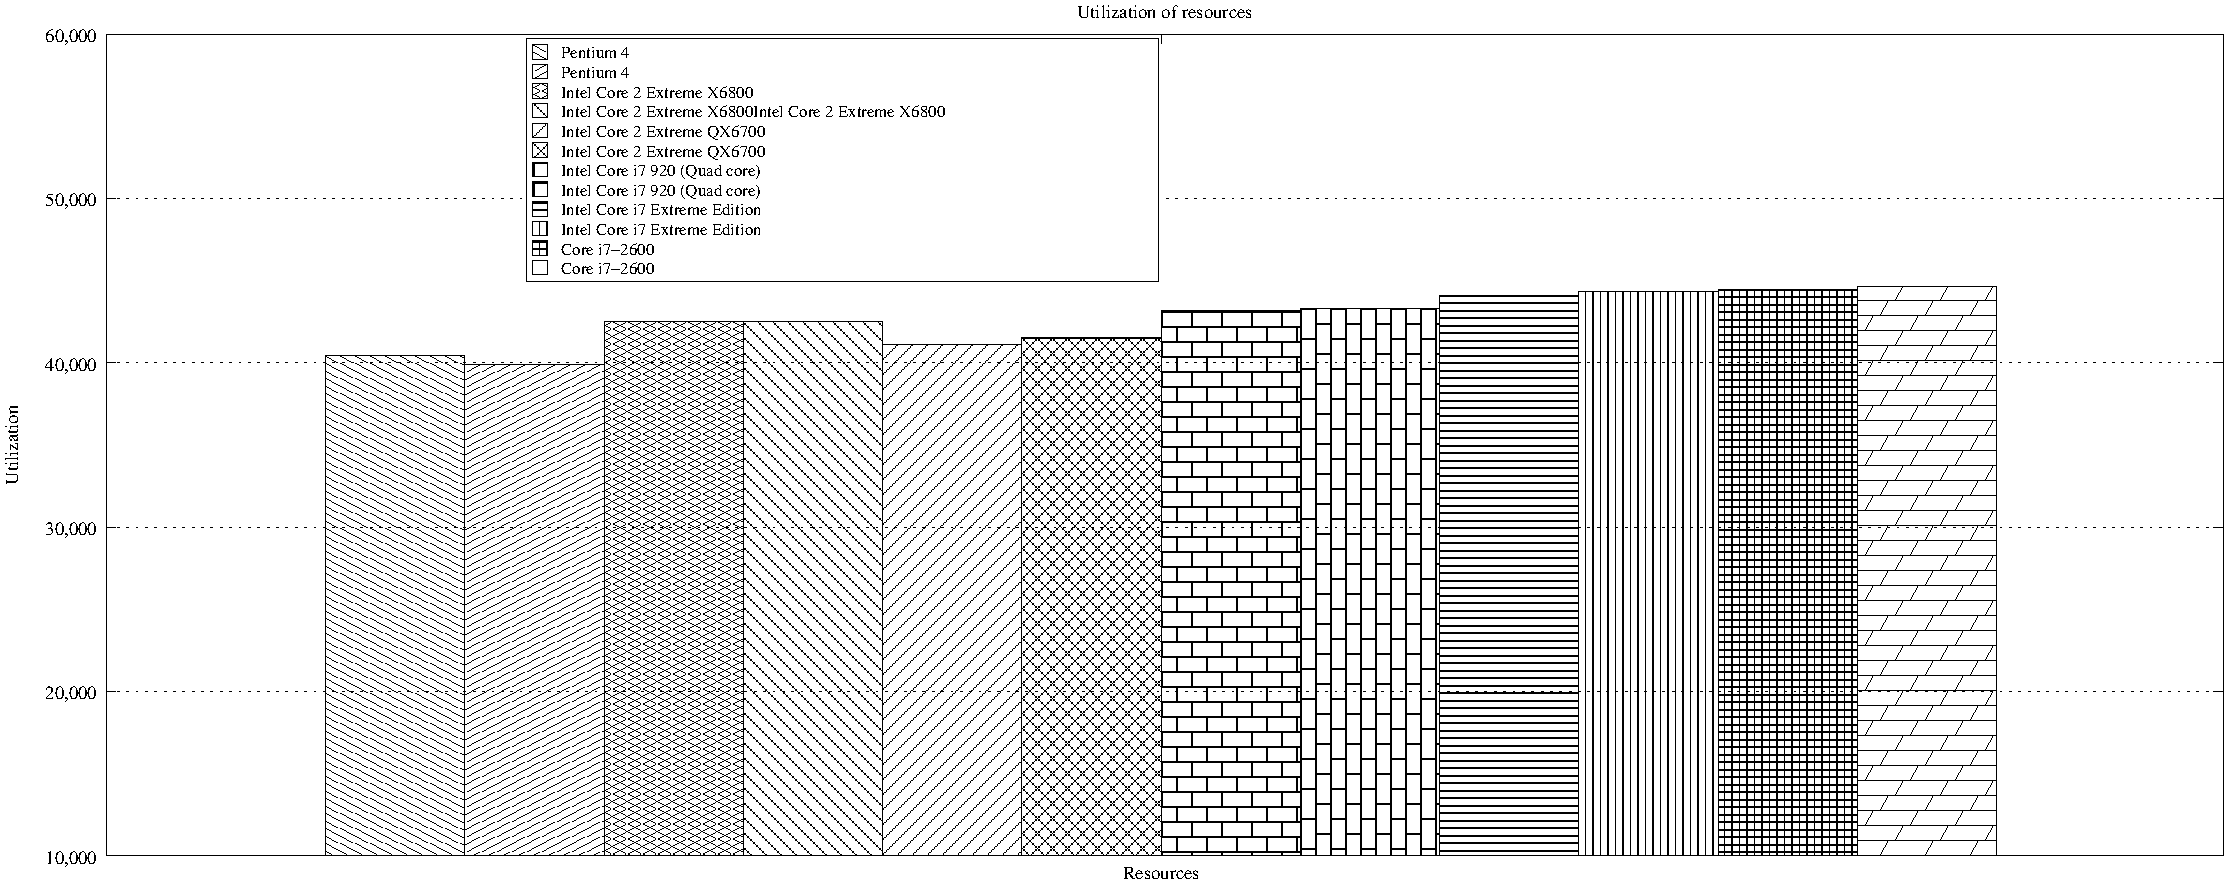
\includegraphics[width=\textwidth]{imgs/case2DAS}
    \caption{Workload 1 (DAS-2)}
\end{figure}
\end{frame}

\begin{frame}
\frametitle{3. Experiment: Introducing job type constraint}
 \begin{figure}[h]
\centering
    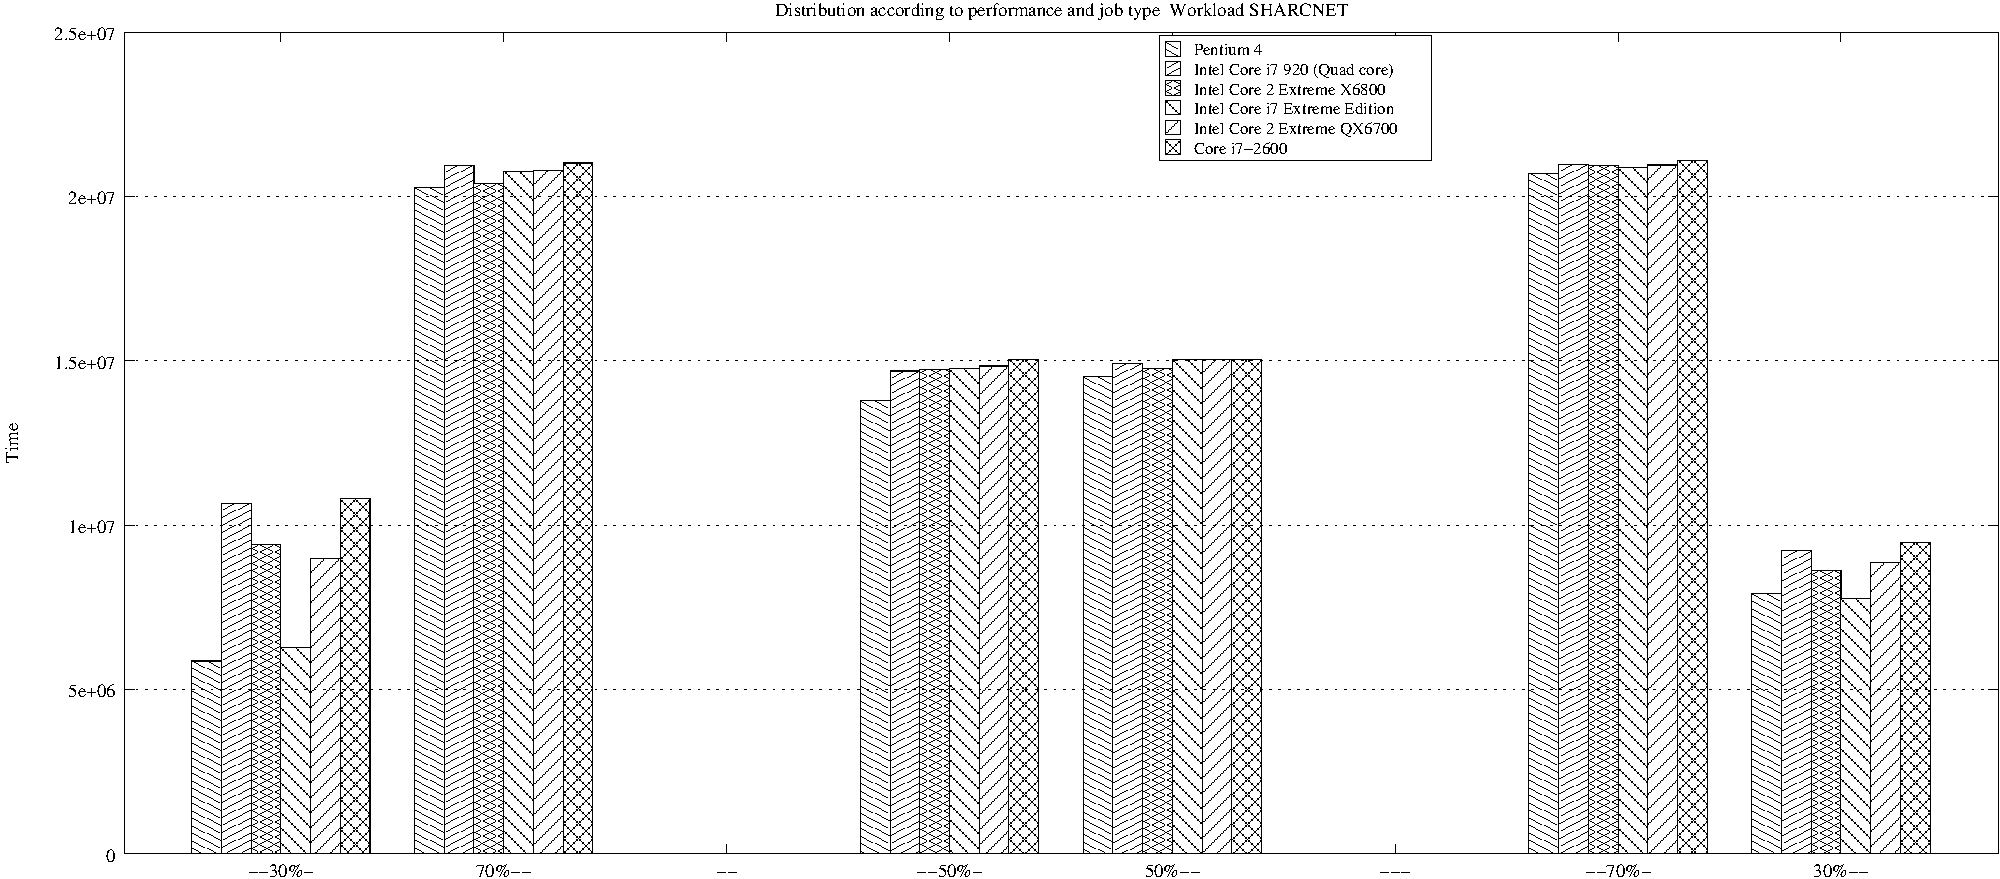
\includegraphics[width=1.0\columnwidth]{imgs/case3_SHARCNET}
    \caption{Performance under Job type constraint, SHARCNET Workload}
\label{jobtype1}
\end{figure}
\end{frame}

\begin{frame}
\frametitle{3. Experiment: Introducing job type constraint}
\begin{figure}[h]
\centering
    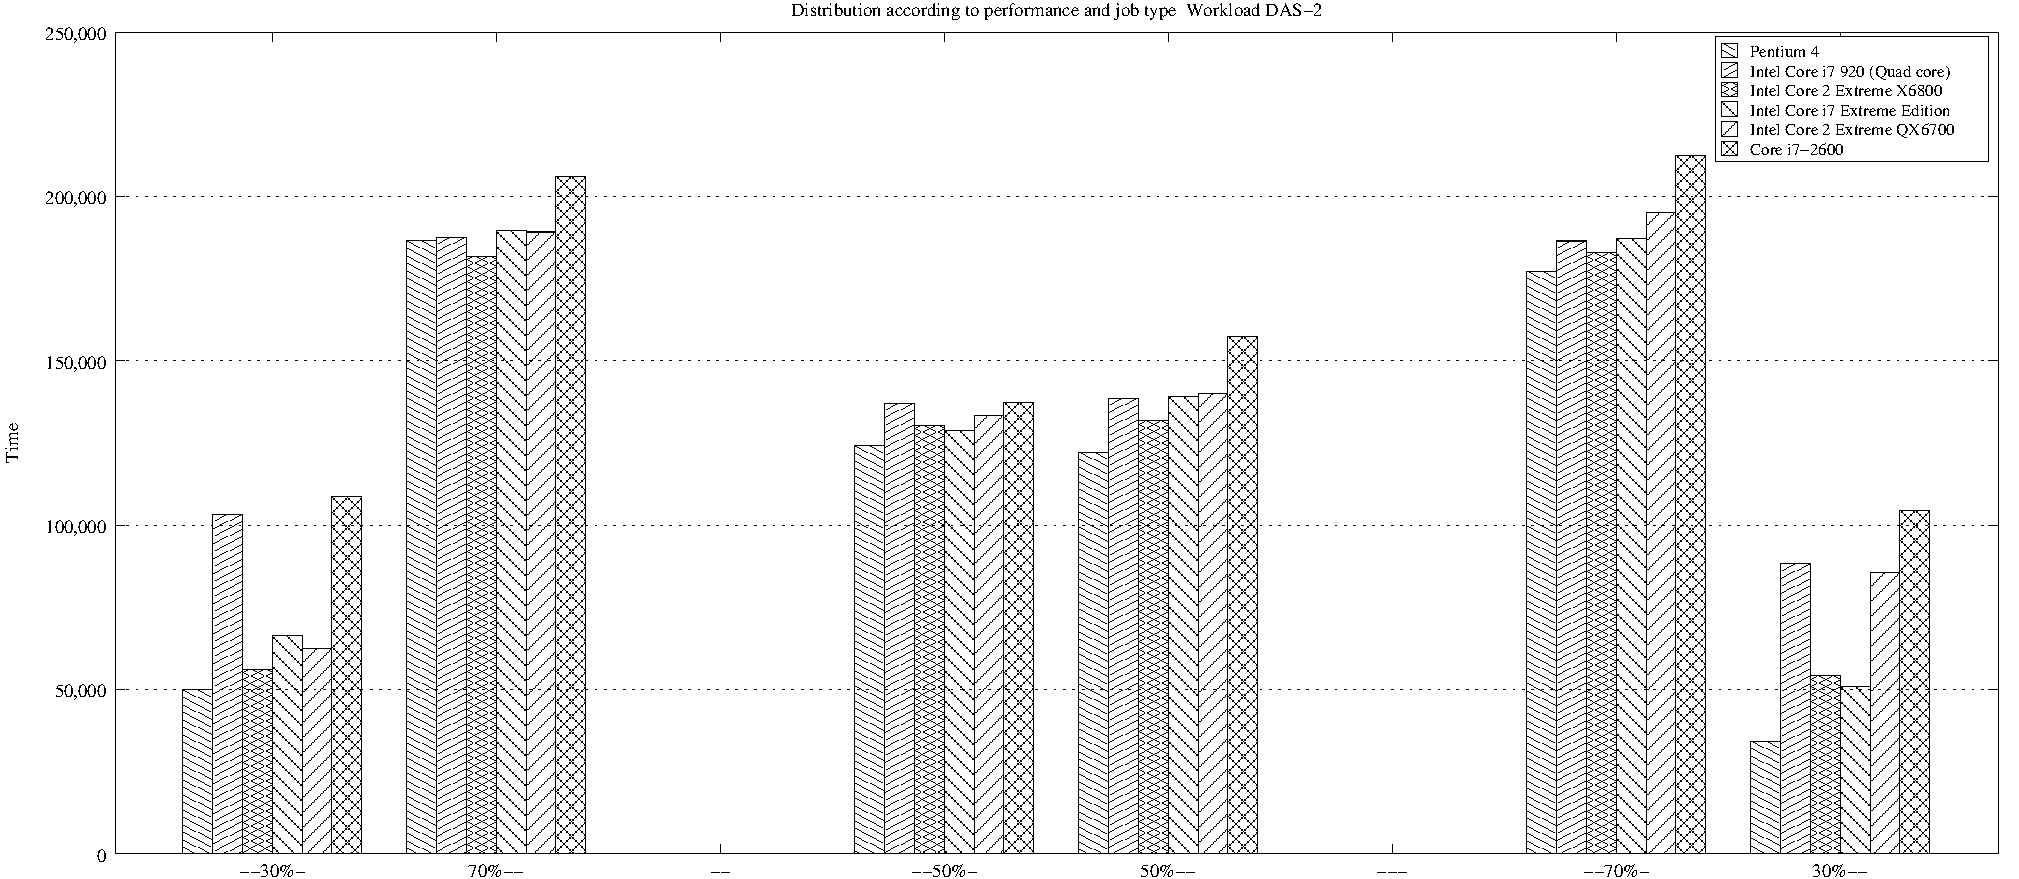
\includegraphics[width=1.0\columnwidth]{imgs/case3_DAS}
    \caption{Performance under Job type constraint, DAS-2 Workload}
\label{jobtype2}
\end{figure}
\end{frame}


\begin{frame}
\frametitle{4. Experiment: Introducing pricing model and precedence constraint}
\begin{table}[ht]
\caption{Resource Utilization after introduction of Job constraint and pricing model Workload 6 (SHARCNET)}
\scalebox{0.45}{
\begin{tabular}{|l|l|r|r|r|r|r|}
    \hline \hline
ID	&	Resource	&	Pricing model	&	Execution time	&	Makespan \%age	&	Actual utilized time	&	Utilization \%age	\\	\hline
1	&	Pentium 4	&	0.05	&	12048592.25	&	98.01	&	11813044.19	&	98.04	\\	\hline
2	&	Pentium 4	&	0.05	&	12163752.56	&	98.95	&	11300235.12	&	92.90	\\	\hline
3	&	Pentium 4	&	0.05	&	12164478.67	&	98.95	&	11686679.20	&	96.07	\\	\hline
4	&	Intel Core i7 920 (Quad core)	&	0.1	&	12046834.85	&	97.99	&	11272379.33	&	93.57	\\	\hline
5	&	Intel Core i7 920 (Quad core)	&	0.1	&	12047842.36	&	98.00	&	11749485.96	&	97.52	\\	\hline
6	&	Intel Core 2 Extreme X6800	&	0.09	&	12048727.00	&	98.01	&	11734951.47	&	97.39	\\	\hline
7	&	Intel Core 2 Extreme X6800	&	0.09	&	12160673.18	&	98.92	&	11776008.86	&	96.83	\\	\hline
8	&	Intel Core i7 Extreme Edition	&	0.15	&	12162928.27	&	98.94	&	11422999.16	&	93.91	\\	\hline
9	&	Intel Core i7 Extreme Edition	&	0.15	&	12160661.70	&	98.92	&	11777797.37	&	96.85	\\	\hline
10	&	Intel Core 2 Extreme QX6700	&	0.165	&	12160968.73	&	98.92	&	11864565.48	&	97.56	\\	\hline
11	&	Intel Core 2 Extreme QX6700	&	0.165	&	12156329.05	&	98.89	&	11976902.34	&	98.52	\\	\hline
12	&	Intel Core 2 Extreme QX6700	&	0.165	&	12160817.18	&	98.92	&	11727719.11	&	96.43	\\	\hline
13	&	Intel Core 2 Extreme QX6700	&	0.165	&	12160965.55	&	98.92	&	11931317.99	&	98.11	\\	\hline
14	&	Core i7-2600	&	0.18	&	12293364.46	&	100.00	&	11959913.00	&	97.28	\\	\hline
15	&	Core i7-2600	&	0.18	&	12161210.37	&	98.92	&	12059303.00	&	99.16	\\	\hline \hline
\end{tabular}
}
\label{tab:sharccase4}
\end{table}
\end{frame}

\begin{frame}
\frametitle{4. Experiment: Introducing pricing model and precedence constraint}
\begin{table}[h]
\caption{Resource Utilization after introduction of Job constraint and pricing model Workload 5 (DAS-2)}
\centering
\scalebox{0.45}{
    \begin{tabular}{|l|l|r|r|r|r|r|}
    \hline \hline
ID	&	Resource	&	Pricing model	&	Execution time	&	Makespan \%age	&	Actual utilized time	&	Utilization \%age	\\	\hline
1	&	Pentium 4	&	0.05	&	307118.82	&	99.20	&	280545.30	&	91.34	\\	\hline
2	&	Pentium 4	&	0.05	&	301366.18	&	97.34	&	270360.92	&	89.71	\\	\hline
3	&	Pentium 4	&	0.05	&	300697.12	&	97.12	&	270477.22	&	89.95	\\	\hline
4	&	Intel Core i7 920 (Quad core)	&	0.1	&	307367.74	&	99.28	&	273357.18	&	88.93	\\	\hline
5	&	Intel Core i7 920 (Quad core)	&	0.1	&	307456.72	&	99.31	&	283748.63	&	92.28	\\	\hline
6	&	Intel Core 2 Extreme X6800	&	0.09	&	305703.06	&	98.74	&	269904.98	&	88.28	\\	\hline
7	&	Intel Core 2 Extreme X6800	&	0.09	&	305227.13	&	98.59	&	276089.83	&	90.45	\\	\hline
8	&	Intel Core i7 Extreme Edition	&	0.15	&	305428.16	&	98.65	&	288772.30	&	94.54	\\	\hline
9	&	Intel Core i7 Extreme Edition	&	0.15	&	303222.35	&	97.94	&	278433.59	&	91.82	\\	\hline
10	&	Intel Core 2 Extreme QX6700	&	0.165	&	309606.43	&	100.00	&	291890.84	&	94.27	\\	\hline
11	&	Intel Core 2 Extreme QX6700	&	0.165	&	309296.74	&	99.90	&	291225.75	&	94.15	\\	\hline
12	&	Intel Core 2 Extreme QX6700	&	0.165	&	305602.29	&	98.71	&	288181.42	&	94.29	\\	\hline
13	&	Intel Core 2 Extreme QX6700	&	0.165	&	303673.86	&	98.08	&	297436.40	&	97.94	\\	\hline
14	&	Core i7-2600	&	0.18	&	308464.86	&	99.63	&	303151.00	&	98.27	\\	\hline
15	&	Core i7-2600	&	0.18	&	308339.70	&	99.59	&	303203.00	&	98.33	\\	\hline \hline
\end{tabular}
}
\label{tab:dascasse4}
\end{table}
\end{frame}


\begin{frame}
\frametitle{5. Experiment with all constraints}
\begin{table}[h]
\centering
\caption{Resource Utilization under all constraints on Workload 7 (DAS-2)}
\scalebox{0.45}{
\begin{tabular}{|l|l|r|r|r|r|r|}
\hline \hline
ID	&	Resource	&	Pricing model	&	Execution time	&	Makespan \%age	&	Actual utilized time	&	Utilization \%age	\\	\hline
1	&	Pentium 4	&	0.05	&	388054.55346	&	95.31	&	337986.508894	&	87.10	\\	\hline
3	&	Intel Core i7 920 (Quad core)	&	0.1	&	390646.860537	&	95.95	&	362241.059321	&	92.72	\\	\hline
5	&	Intel Core 2 Extreme X6800	&	0.09	&	391917.860219	&	96.26	&	357671.610452	&	91.26	\\	\hline
7	&	Intel Core i7 Extreme Edition	&	0.15	&	389061.135613	&	95.56	&	367173.559685	&	94.37	\\	\hline
9	&	Intel Core 2 Extreme QX6700	&	0.165	&	389834.143125	&	95.75	&	368452.037427	&	94.51	\\	\hline
11	&	Core i7-2600	&	0.18	&	394967.616183	&	97.01	&	365376	&	92.50	\\	\hline
2	&	Pentium 4	&	0.05	&	407130.811479	&	100.00	&	362875.39219	&	89.12	\\	\hline
4	&	Intel Core i7 920 (Quad core)	&	0.1	&	406698.612175	&	99.89	&	343454.864029	&	84.44	\\	\hline
6	&	Intel Core 2 Extreme X6800	&	0.09	&	403146.303747	&	99.02	&	348012.012859	&	86.32	\\	\hline
8	&	Intel Core i7 Extreme Edition	&	0.15	&	402622.406754	&	98.89	&	378981.878416	&	94.12	\\	\hline
10	&	Intel Core 2 Extreme QX6700	&	0.165	&	405572.293961	&	99.62	&	385571.358202	&	95.06	\\	\hline
12	&	Core i7-2600	&	0.18	&	394268.616183	&	96.84	&	374894	&	95.08	\\	\hline \hline
\end{tabular}
}
\label{case5das}
\end{table}
\end{frame}

\begin{frame}
\frametitle{5. Experiment with all constraints}
\begin{table}[h]
\centering
\caption{Resource Utilization under all constraints on Workload 8 (SHARCNET) }
\scalebox{0.45}{
    \begin{tabular}{|l|l|r|r|r|r|r|}
    \hline \hline
ID	&	Resource	&	Pricing model	&	Execution time	&	Makespan \%age	&	Actual utilized time	&	Utilization \%age	\\	\hline
1	&	Pentium 4	&	0.05	&	15856966.328786	&	99.65	&	14643863.906402	&	92.34	\\	\hline
3	&	Intel Core i7 920 (Quad core)	&	0.1	&	15777189.495383	&	99.14	&	14224208.443954	&	90.15	\\	\hline
5	&	Intel Core 2 Extreme X6800	&	0.09	&	15777954.142035	&	99.15	&	14347179.713218	&	90.93	\\	\hline
7	&	Intel Core i7 Extreme Edition	&	0.15	&	15853934.301256	&	99.63	&	14962167.332284	&	94.37	\\	\hline
9	&	Intel Core 2 Extreme QX6700	&	0.165	&	15855065.258749	&	99.63	&	14971170.083674	&	94.42	\\	\hline
11	&	Core i7-2600	&	0.18	&	15807884.835386	&	99.34	&	14039647	&	88.81	\\	\hline
2	&	Pentium 4	&	0.05	&	15855945.977623	&	99.64	&	15192585.514258	&	95.81	\\	\hline
4	&	Intel Core i7 920 (Quad core)	&	0.1	&	15856889.388767	&	99.65	&	15492772.72683	&	97.70	\\	\hline
6	&	Intel Core 2 Extreme X6800	&	0.09	&	15856577.788845	&	99.64	&	15509484.322644	&	97.81	\\	\hline
8	&	Intel Core i7 Extreme Edition	&	0.15	&	15808788.880171	&	99.34	&	15123906.518069	&	95.66	\\	\hline
10	&	Intel Core 2 Extreme QX6700	&	0.165	&	15913317.542563	&	100.00	&	15439774.23157	&	97.02	\\	\hline
12	&	Core i7-2600	&	0.18	&	15884947.971385	&	99.82	&	15685884	&	98.74	\\	\hline \hline
\end{tabular}
}
\label{case5sha}
\end{table}
\end{frame}

\begin{frame}
 \frametitle{5. Experiment with all constraints}
\vspace{-10pt}
\begin{table}[h]
\centering
\caption{\tiny Resource Utilization under all constraints on Workload (SHARCNET) with 24 resources }
\scalebox{0.45}{
\vspace{-5pt}
    \begin{tabular}{|l|l|r|r|r|r|r|}
    \hline \hline
ID	&	Resource	&	Pricing model	&	Execution time	&	Makespan \%age	&	Actual utilized time	&	Utilization Percentage	\\	\hline
1	&	Pentium 4	&	0.05	&	8243698.72	&	99.49	&	7556234.16	&	91.66	\\	\hline
2	&	Pentium 4	&	0.05	&	7275262.72	&	87.81	&	6253412.08	&	85.95	\\	\hline
3	&	Intel Core i7 920 (Quad core)	&	0.1	&	7682671.48	&	92.72	&	6326204.11	&	82.34	\\	\hline
4	&	Intel Core i7 920 (Quad core)	&	0.1	&	8233315.82	&	99.37	&	7351339.16	&	89.28	\\	\hline
5	&	Intel Core 2 Extreme X6800	&	0.09	&	8117606.74	&	97.97	&	7269743.03	&	89.55	\\	\hline
6	&	Intel Core 2 Extreme X6800	&	0.09	&	8118002.88	&	97.98	&	7072373.18	&	87.11	\\	\hline
7	&	Intel Core i7 Extreme Edition	&	0.15	&	8117468.76	&	97.97	&	7183725.78	&	88.49	\\	\hline
8	&	Intel Core i7 Extreme Edition	&	0.15	&	8244584.64	&	99.50	&	7426916.89	&	90.08	\\	\hline
9	&	Intel Core 2 Extreme QX6700	&	0.165	&	8117904.66	&	97.98	&	7220275.87	&	88.94	\\	\hline
10	&	Intel Core 2 Extreme QX6700	&	0.165	&	8119335.22	&	97.99	&	7202661.19	&	88.70	\\	\hline
11	&	Core i7-2600	&	0.18	&	8229761.81	&	99.33	&	7763631	&	94.33	\\	\hline
12	&	Core i7-2600	&	0.18	&	8244728.91	&	99.51	&	7615311	&	92.36	\\	\hline
13	&	Pentium 4	&	0.05	&	8119374.38	&	97.99	&	7906705.97	&	97.38	\\	\hline
14	&	Pentium 4	&	0.05	&	8231574.39	&	99.35	&	7705017.38	&	93.60	\\	\hline
15	&	Intel Core i7 920 (Quad core)	&	0.1	&	8229150.06	&	99.32	&	7628743.04	&	92.70	\\	\hline
16	&	Intel Core i7 920 (Quad core)	&	0.1	&	8117134.83	&	97.97	&	7339766.91	&	90.42	\\	\hline
17	&	Intel Core 2 Extreme X6800	&	0.09	&	8244402.12	&	99.50	&	7126312.76	&	86.43	\\	\hline
18	&	Intel Core 2 Extreme X6800	&	0.09	&	8120187.28	&	98.00	&	7600934.79	&	93.60	\\	\hline
19	&	Intel Core i7 Extreme Edition	&	0.15	&	8285650.01	&	100.00	&	8151742.16	&	98.38	\\	\hline
20	&	Intel Core i7 Extreme Edition	&	0.15	&	8230477.53	&	99.33	&	7746832.68	&	94.12	\\	\hline
21	&	Intel Core 2 Extreme QX6700	&	0.165	&	8232608.55	&	99.36	&	7776374.29	&	94.45	\\	\hline
22	&	Intel Core 2 Extreme QX6700	&	0.165	&	8230191.41	&	99.33	&	7517359.04	&	91.33	\\	\hline
23	&	Core i7-2600	&	0.18	&	8244461.91	&	99.50	&	7950420	&	96.43	\\	\hline
24	&	Core i7-2600	&	0.18	&	8244329.91	&	99.50	&	7745014	&	93.94	\\	\hline
\end{tabular}
}
\label{case5sha24}
\end{table}
\end{frame}


\comment{
\begin{frame}
 \frametitle{ISRO Bio-Diversity Dataset}
\begin{figure}[t]
	\centering
	\subfigure[]
	{
		\includegraphics[scale=\figscale]{Category1.png}
		\label{fig:cata}
	}
	\subfigure[]
	{
		\includegraphics[scale=\figscale]{Category2.png}
		\label{fig:catb}
	}
	\subfigure[]
	{
		\includegraphics[scale=\figscale]{Category4.png}
		\label{fig:catc}
	}
	%\\
	\subfigure[]
	{
		\includegraphics[scale=\figscale]{Category5.png}
		\label{fig:catd}
	}
	%\subfloat[]
	%{
	%	\includegraphics[scale=\figscale]{Category7.png}
	%	\label{fig:cate}
	%}
	%\subfloat[]
	%{
	%	\includegraphics[scale=\figscale]{Category8.png}
	%	\label{fig:catf}
	%}						
	\caption{Categories of the mined subgraphs.}
	\label{fig:category}
\end{figure}
\end{frame}

}
\section[Conclusions]{Conclusions}
\begin{frame}
\frametitle{Conclusions}
\Fontdi
\begin{itemize}
  \item This work provides a flexible scheduler keeping multiple objectives into consideration. 
  \item The scheduler module yields best scheduling strategies on various parameters in a pareto front. This is upto grid administrator and dynamic grid environment to choose a scheduling strategy of its choice.
  \item The scheduler is scalable with resources and can process an infinite queue of jobs. 
  \item The scheduler responded well with the change of constraints and behaviour of grid and job model. 
  \item All resources have adhered to the makespan, energy efficiency, QoS and utilization rate is also high inspite of constraints imposed.
\end{itemize}
\end{frame}


\begin{frame}[allowframebreaks]
  \frametitle{References}
  \bibliographystyle{alpha}
  \Fontci
  \bibliography{refall}
\end{frame}

\begin{frame}
 \begin{center}
  \Fontti
  THANK YOU!!
 \end{center}
\end{frame}

\section{Supplementary Info}

%\subsection*{Significance Testing}
\begin{frame}[label=supplement1]
 \frametitle{Makespan}
\begin{figure}[t]
\centering
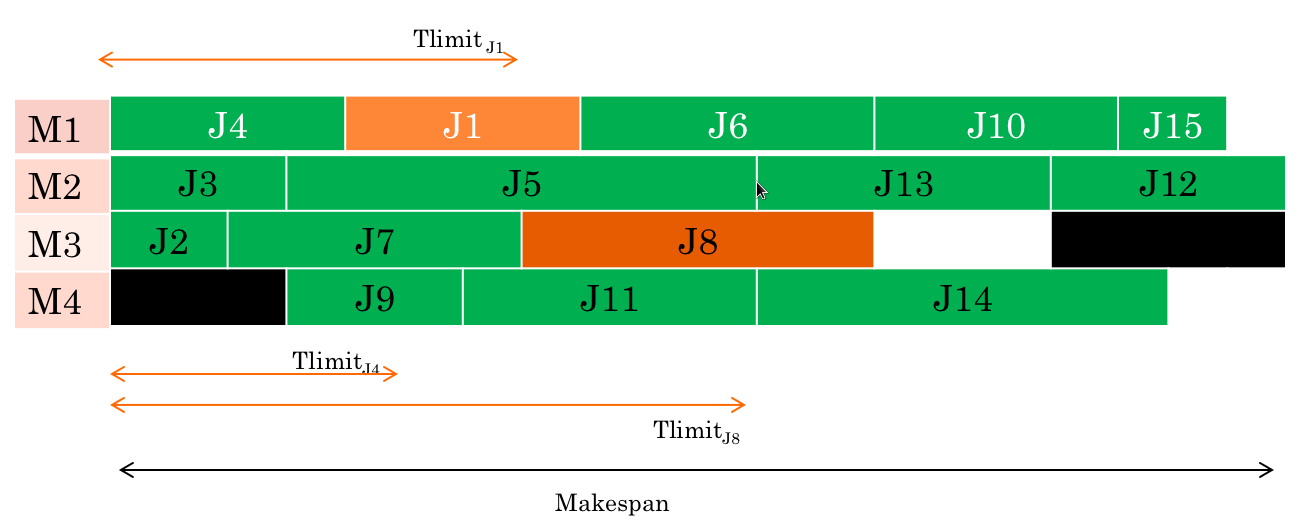
\includegraphics[width=0.90\textwidth]{imgs/makespan}
\vspace{-7pt}
\caption{Makespan example}
\end{figure}
\begin{itemize}
	\item The completion time for the entire set of Jobs on all resources  \hyperlink{back1}{\beamerbutton{back}} \hyperlink{mkspn1}{\beamerbutton{objectives}}.
\end{itemize}
\end{frame}

\begin{frame}[label=supplement2]
 \frametitle{Grid computing (Defn)} 
\begin{itemize}
	\item "A  Grid  is  a  collection  of  distributed  computing resources  available  over  a  local  or  wide  area  network that appears to an end user or application as one large virtual computing system." - IBM 
	\item "Conceptually, a grid is quite simple. It is a collection of  computing  resources  that  perform  tasks.  In  its simplest form, a grid appears to users as a large system that  provides  a  single  point  of  access  to  powerful distributed resources." - Sun 
	\item "Grid computing is computing as a utility - you do not care  where  data  resides,  or  what  computer  processes  your  requests.  Analogous  to  the  way  utilities  work, clients request information or computation and have it delivered  -  as  much  as  they  want,  and  whenever  they want." - Oracle \hyperlink{back2}{\beamerbutton{back}}
\end{itemize}
\end{frame}

\begin{frame}[label=supplement3]
 \frametitle{Types of Grid} 
\begin{itemize} 
\item \textbf{Computational Grid:} A computational grid is a collection of distributed computing resources, within or across locations that are combined
to act as a unified computing resource.
\item  \textbf{Data Grid:} Data grid primarily deals with providing services and infrastructure for distributed data-intensive applications that need to access, transfer
and modify massive datasets stored in distributed storage resources \cite{chervenak2000data}.
\vspace{-2pt}
\hyperlink{back2}{\beamerbutton{back}}
\end{itemize}
\end{frame}

\begin{frame}[label=nds]
 \frametitle{Non-dominating points}
\begin{itemize} 
	\item A chromosome $a$ is said to be dominated by chromosome $b$ iff $\forall i \in \{1,2,\ldots,k\}: f_i(a) \leq f_i(b)$ and $\exists i \in \{1,2,\ldots,k\}: f_i(a) < f_i(b)$.
	\item A chromosome $a$ is said to be Non-dominated if there does not exist any chromosome $b\in \mathbb{V}$ search space that dominates $a$. A set of such non-dominated chromosome in objective space is called pareto optimal front. \hyperlink{back4}{\beamerbutton{back}}
\end{itemize}
\end{frame}

\begin{frame}[label=nds1]
 \frametitle{Non-dominating points}
\begin{figure}[h]
 \begin{center}
  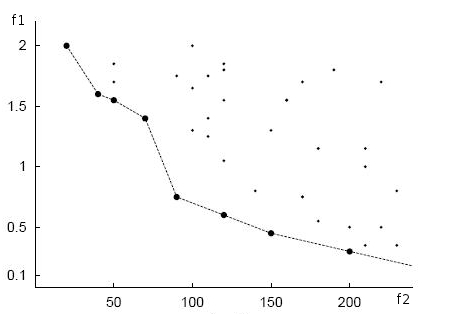
\includegraphics[width=0.70\textwidth]{imgs/nondom}
 \end{center}
  \caption{An example of non-dominating points in \emph{2-d} \hyperlink{back4}{\beamerbutton{back}} \hyperlink{chromosomemod}{\beamerbutton{rank}}}
\end{figure}
\end{frame}

\begin{frame}[label=paretofrnt]
 \frametitle{Pareto front}
\begin{figure}[t]
 \begin{center}
  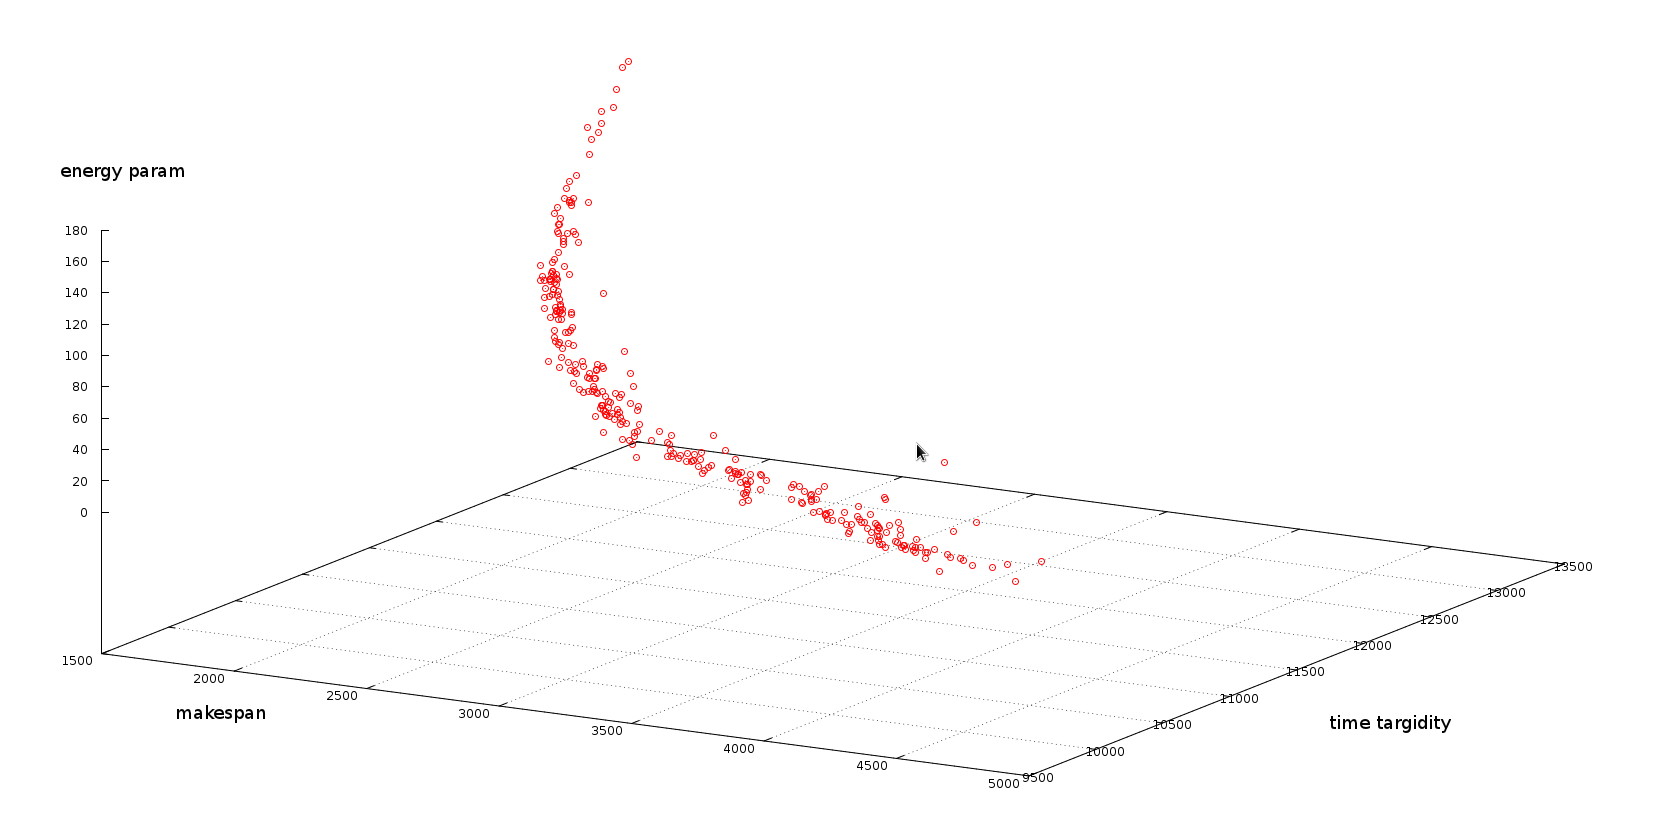
\includegraphics[width=0.90\textwidth]{imgs/pareto}
 \end{center}
  \caption{An example of pareto front from our experiment \hyperlink{back4}{\beamerbutton{back}}}
\end{figure}
\end{frame}

\begin{frame}[label=paretofrnt1]
 \frametitle{Pareto front}
\begin{figure}[t]
 \begin{center}
  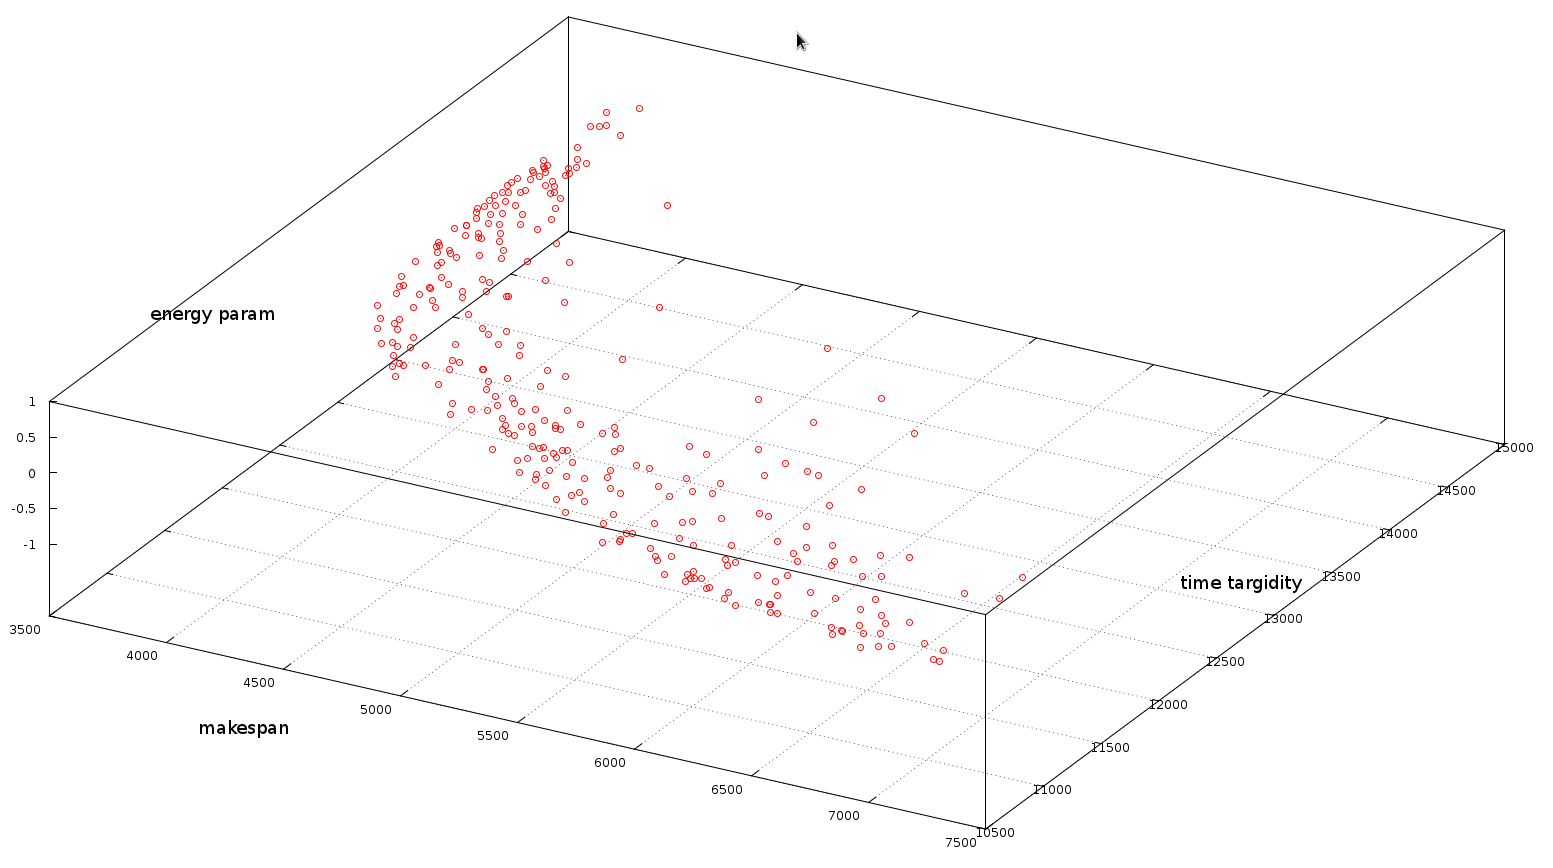
\includegraphics[width=0.90\textwidth]{imgs/pareto2}
 \end{center}
  \caption{An example of pareto front from our experiment \hyperlink{back4}{\beamerbutton{back}}}
\end{figure}
\end{frame}

\begin{frame}[label=paretofrnt1]
 \frametitle{Pareto front}
\begin{figure}[t]
 \begin{center}
  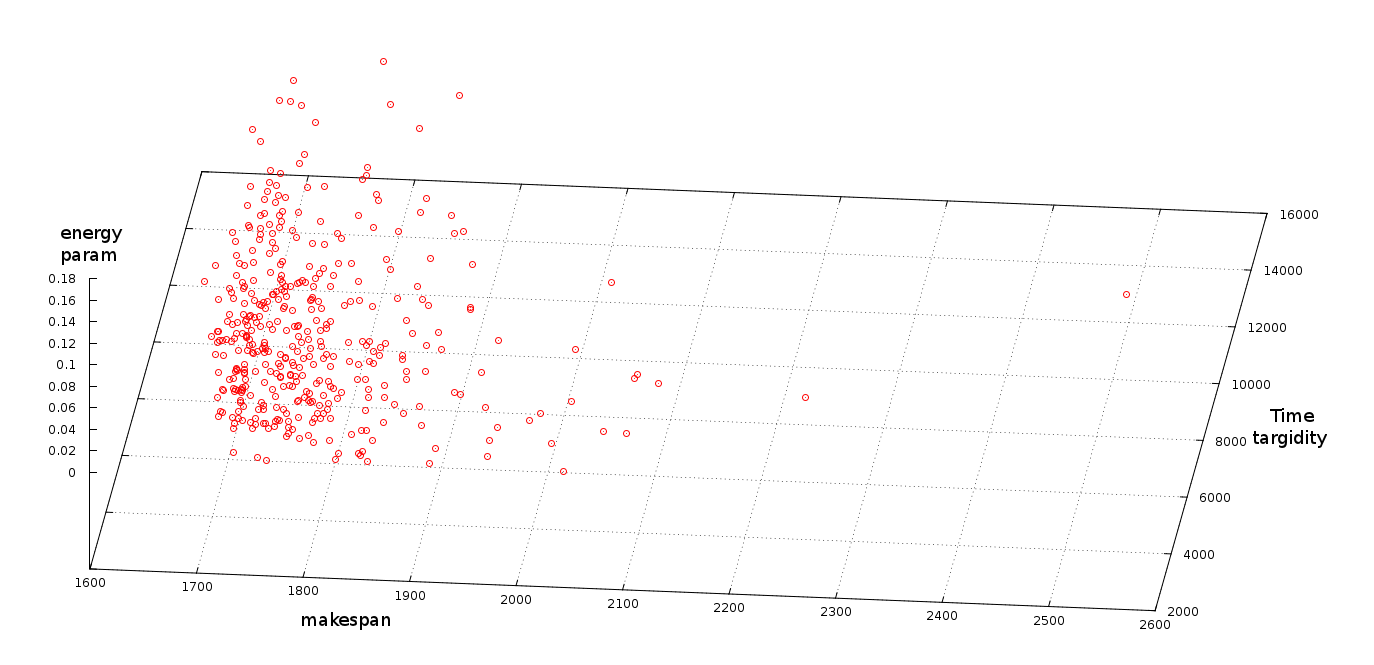
\includegraphics[width=0.90\textwidth]{imgs/pareto3}
 \end{center}
  \caption{An example of pareto front from our experiment \hyperlink{back4}{\beamerbutton{back}}}
\end{figure}
\end{frame}

\begin{frame}[label=paretofrnt1]
 \frametitle{Pareto front}
\begin{figure}[t]
 \begin{center}
  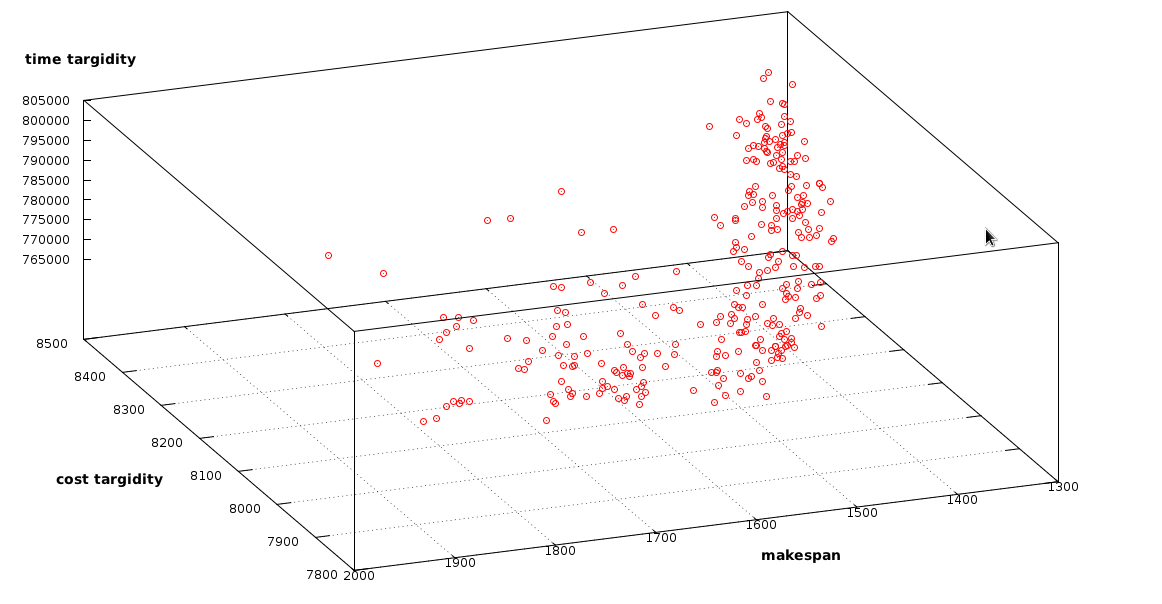
\includegraphics[width=0.90\textwidth]{imgs/pareto4}
 \end{center}
  \caption{An example of pareto front from our experiment \hyperlink{back4}{\beamerbutton{back}}}
\end{figure}
\end{frame}


\begin{frame}[label=crwd]
 \frametitle{Crowding distance}
\begin{block}
 {Crowding distance} Crowding distance ($dist_x$) of a particular chromosome $x$ in population measures the density of chromosomes surrounding it. \\
\end{block}
\begin{itemize}
\item $dist_x = \sum _{j=1}^{k}\frac{f_j(x_{left})-f_j(x_{right})}{f_j^{max} -f_j^{min}}$\\
where $f_j$ is $j$th objective function, and number of objectives is $k$.
\item A partial order $\prec$ between chromosomes are defined as:\\
$ a \prec b $ if $r_a \prec r_b$\\
or $(r_a = r_b)$ and $(dist_a \succ dist_b)$ \hyperlink{chromosomemod}{\beamerbutton{back}}
\end{itemize}
\end{frame}

\begin{frame}[label=jbgrpeq]
\frametitle{Job grouping; Critical length}
\begin{block}
{Critical length} It denoted as $crit(j)$ refers to the longest distance from $j_{entry}$ to $j_{exit}$ passing through the job $j$. 
\end{block}
{\tiny
The Upward Critical length of job $j$ is the longest distance from $j$ to the exit job $j_{exit}$. It is denoted as $crit_{up}(j)_{<type>}$ where $_{<type>}$ is computational and storage. Upward critical length is computed with the equation~\ref{eq:up1} starting from $j{exit}$ and moving upward towards $j$.
\begin{equation}\label{eq:up1}
crit_{up}(j)_{<type>} = job\_size(j)_{<type>} + max_{j' \in succ(j)}(crit_{up}(j')_{<type>})
\end{equation}
%\begin{equation}\label{eq:up2}
%crit_{up}(j)_{storage} = job\_size(j)_{storage} + max_{j' \in succ(j)}(crit_{up}(j')_{storage})
% \end{equation}
Similarly, the Downward Critical length of job $j$ is the longest distance from the entry job $j_{entry}$ to $j$. It is denoted as $crit_{down}(j)_{<type>}$ where $_{<type>}$ is computational and storage. Downward critical length is computed with the equation~\ref{eq:down1} starting from $j{entry}$ and moving downward towards $j$.
\begin{equation}\label{eq:down1}
crit_{down}(j)_{<type>} = job\_size(j)_{<type>} + max_{j' \in pred(j)}(crit_{down}(j')_{<type>}) 
\end{equation} \hyperlink{jbgrp}{\beamerbutton{algorithm}}
}
\end{frame}

\begin{frame}[label=jbgrp]
 \frametitle{Job Grouping Algorithm \hyperlink{jbgrpeq}{\tiny \beamerbutton{eqn. link}} \hyperlink{jbgrpimg}{\tiny \beamerbutton{back}}}
\vspace{-12pt}
\begin{algorithm}[H]
\caption{\tiny Job grouping}
\Fontvi
\begin{algorithmic}
\REQUIRE { Job pool with DAG representation }
\STATE {Compute $crit_{up}(j)_{<type>}$ for each job $j$   according to the equation ~\ref{eq:up1} }
\STATE {Compute $crit_{down}(j)_{<type>}$ for each job $j$ according to the equation ~\ref{eq:down1} }
\STATE { Compute $crit_{<type>}$ for each job $j$ }
\WHILE { Job $a \in $ job pool exists, where $a$ is unprocessed fine-grained job }
  \STATE { $flag \leftarrow 0$ }
  \WHILE { $a$ is fine-grained job \AND $flag = 0$ }
    \FOR {each $b \in adjacent\_node(a)$ \AND  same type i.e. computational or storage }
	  \STATE { Temporary merge adjacent node $b$ and $a$ to form $t$}
	  \STATE { Calculate new $crit_{up}(t)_{<type>}$ , $crit_{down}(t)_{<type>}$ and $crit(t)_{<type>}$ }
	  \IF {new $crit(t)_{<type>} \leq crit(j_{entry})_{<type>}$ \AND $crit(t)_{<type>}$ is minimum till now }
	      \STATE { $merge\_node$ $\leftarrow b$ }
	  \ENDIF
    \ENDFOR
    \IF { $merge\_node$ is found }
	\STATE { Permanently merge $merge\_node$ with $a$ to form $a'$ }
	\STATE Change parent and child relation accordingly 
	\IF { $a'$ is not fine-grained job}
	    \STATE { $flag\leftarrow 1$ }
	\ENDIF
    \ELSE 
	    \STATE { $flag\leftarrow 1$ }
    \ENDIF
\ENDWHILE
\ENDWHILE
\end{algorithmic}
\label{jobgrouping}
\end{algorithm}
\end{frame}


\subsection*{Key components}
\begin{frame}[label=main2]
 \frametitle{Portal or User Interface} 
\begin{figure}[t]
\centering
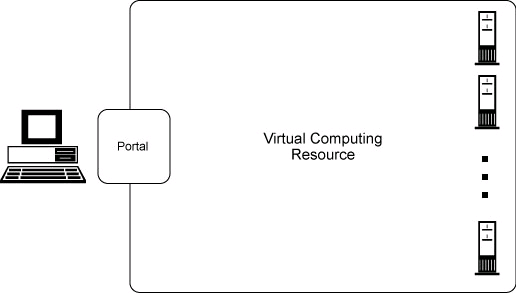
\includegraphics[width=0.95\textwidth]{imgs/key1}
%\caption{A typical view of Grid environment}
\end{figure}
\end{frame}

\begin{frame}[label=main2]
 \frametitle{Grid Security Infrastructure (GSI)} 
\begin{figure}[t]
\centering
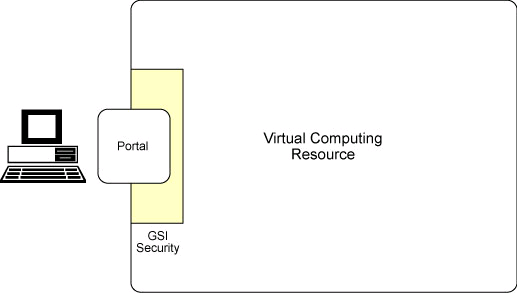
\includegraphics[width=0.95\textwidth]{imgs/key2}
%\caption{A typical view of Grid environment}
\end{figure}
\end{frame}

\begin{frame}[label=main2]
 \frametitle{Broker, Monitoring and Discovery Service} 
\begin{figure}[t]
\centering
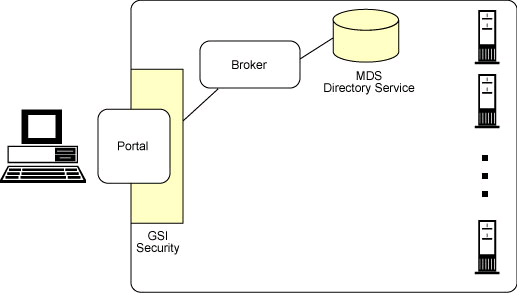
\includegraphics[width=0.95\textwidth]{imgs/key3}
%\caption{A typical view of Grid environment}
\end{figure}
\end{frame}

\begin{frame}[label=main2]
 \frametitle{Scheduler} 
\begin{figure}[t]
\centering
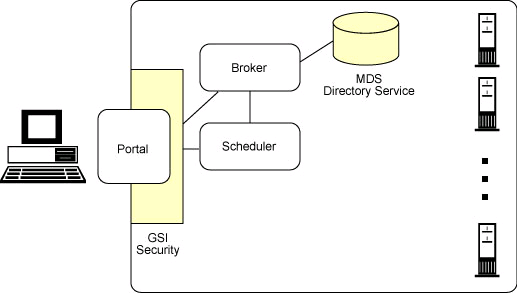
\includegraphics[width=0.95\textwidth]{imgs/key4}
%\caption{A typical view of Grid environment}
\end{figure}
\end{frame}

\begin{frame}[label=main2]
 \frametitle{Data Management} 
\begin{figure}[t]
\centering
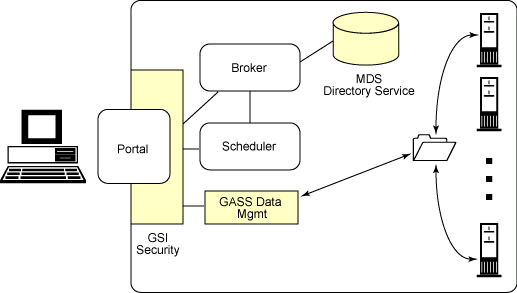
\includegraphics[width=0.95\textwidth]{imgs/key5}
%\caption{A typical view of Grid environment}
\end{figure}
\end{frame}

\begin{frame}[label=main2]
 \frametitle{Dispatcher or Grid Resource Allocation Manager} 
\begin{figure}[t]
\centering
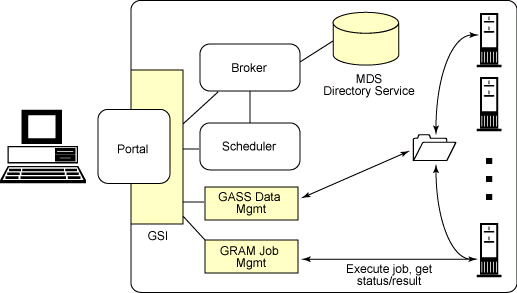
\includegraphics[width=0.95\textwidth]{imgs/key6}
%\caption{A typical view of Grid environment}
\end{figure}
\end{frame}


\end{document}
